\newpage
\begin{tikzpicture}[remember picture, overlay]
	\node [inner sep=0pt, minimum width=\paperwidth, minimum height=\paperheight] at (current page.center) {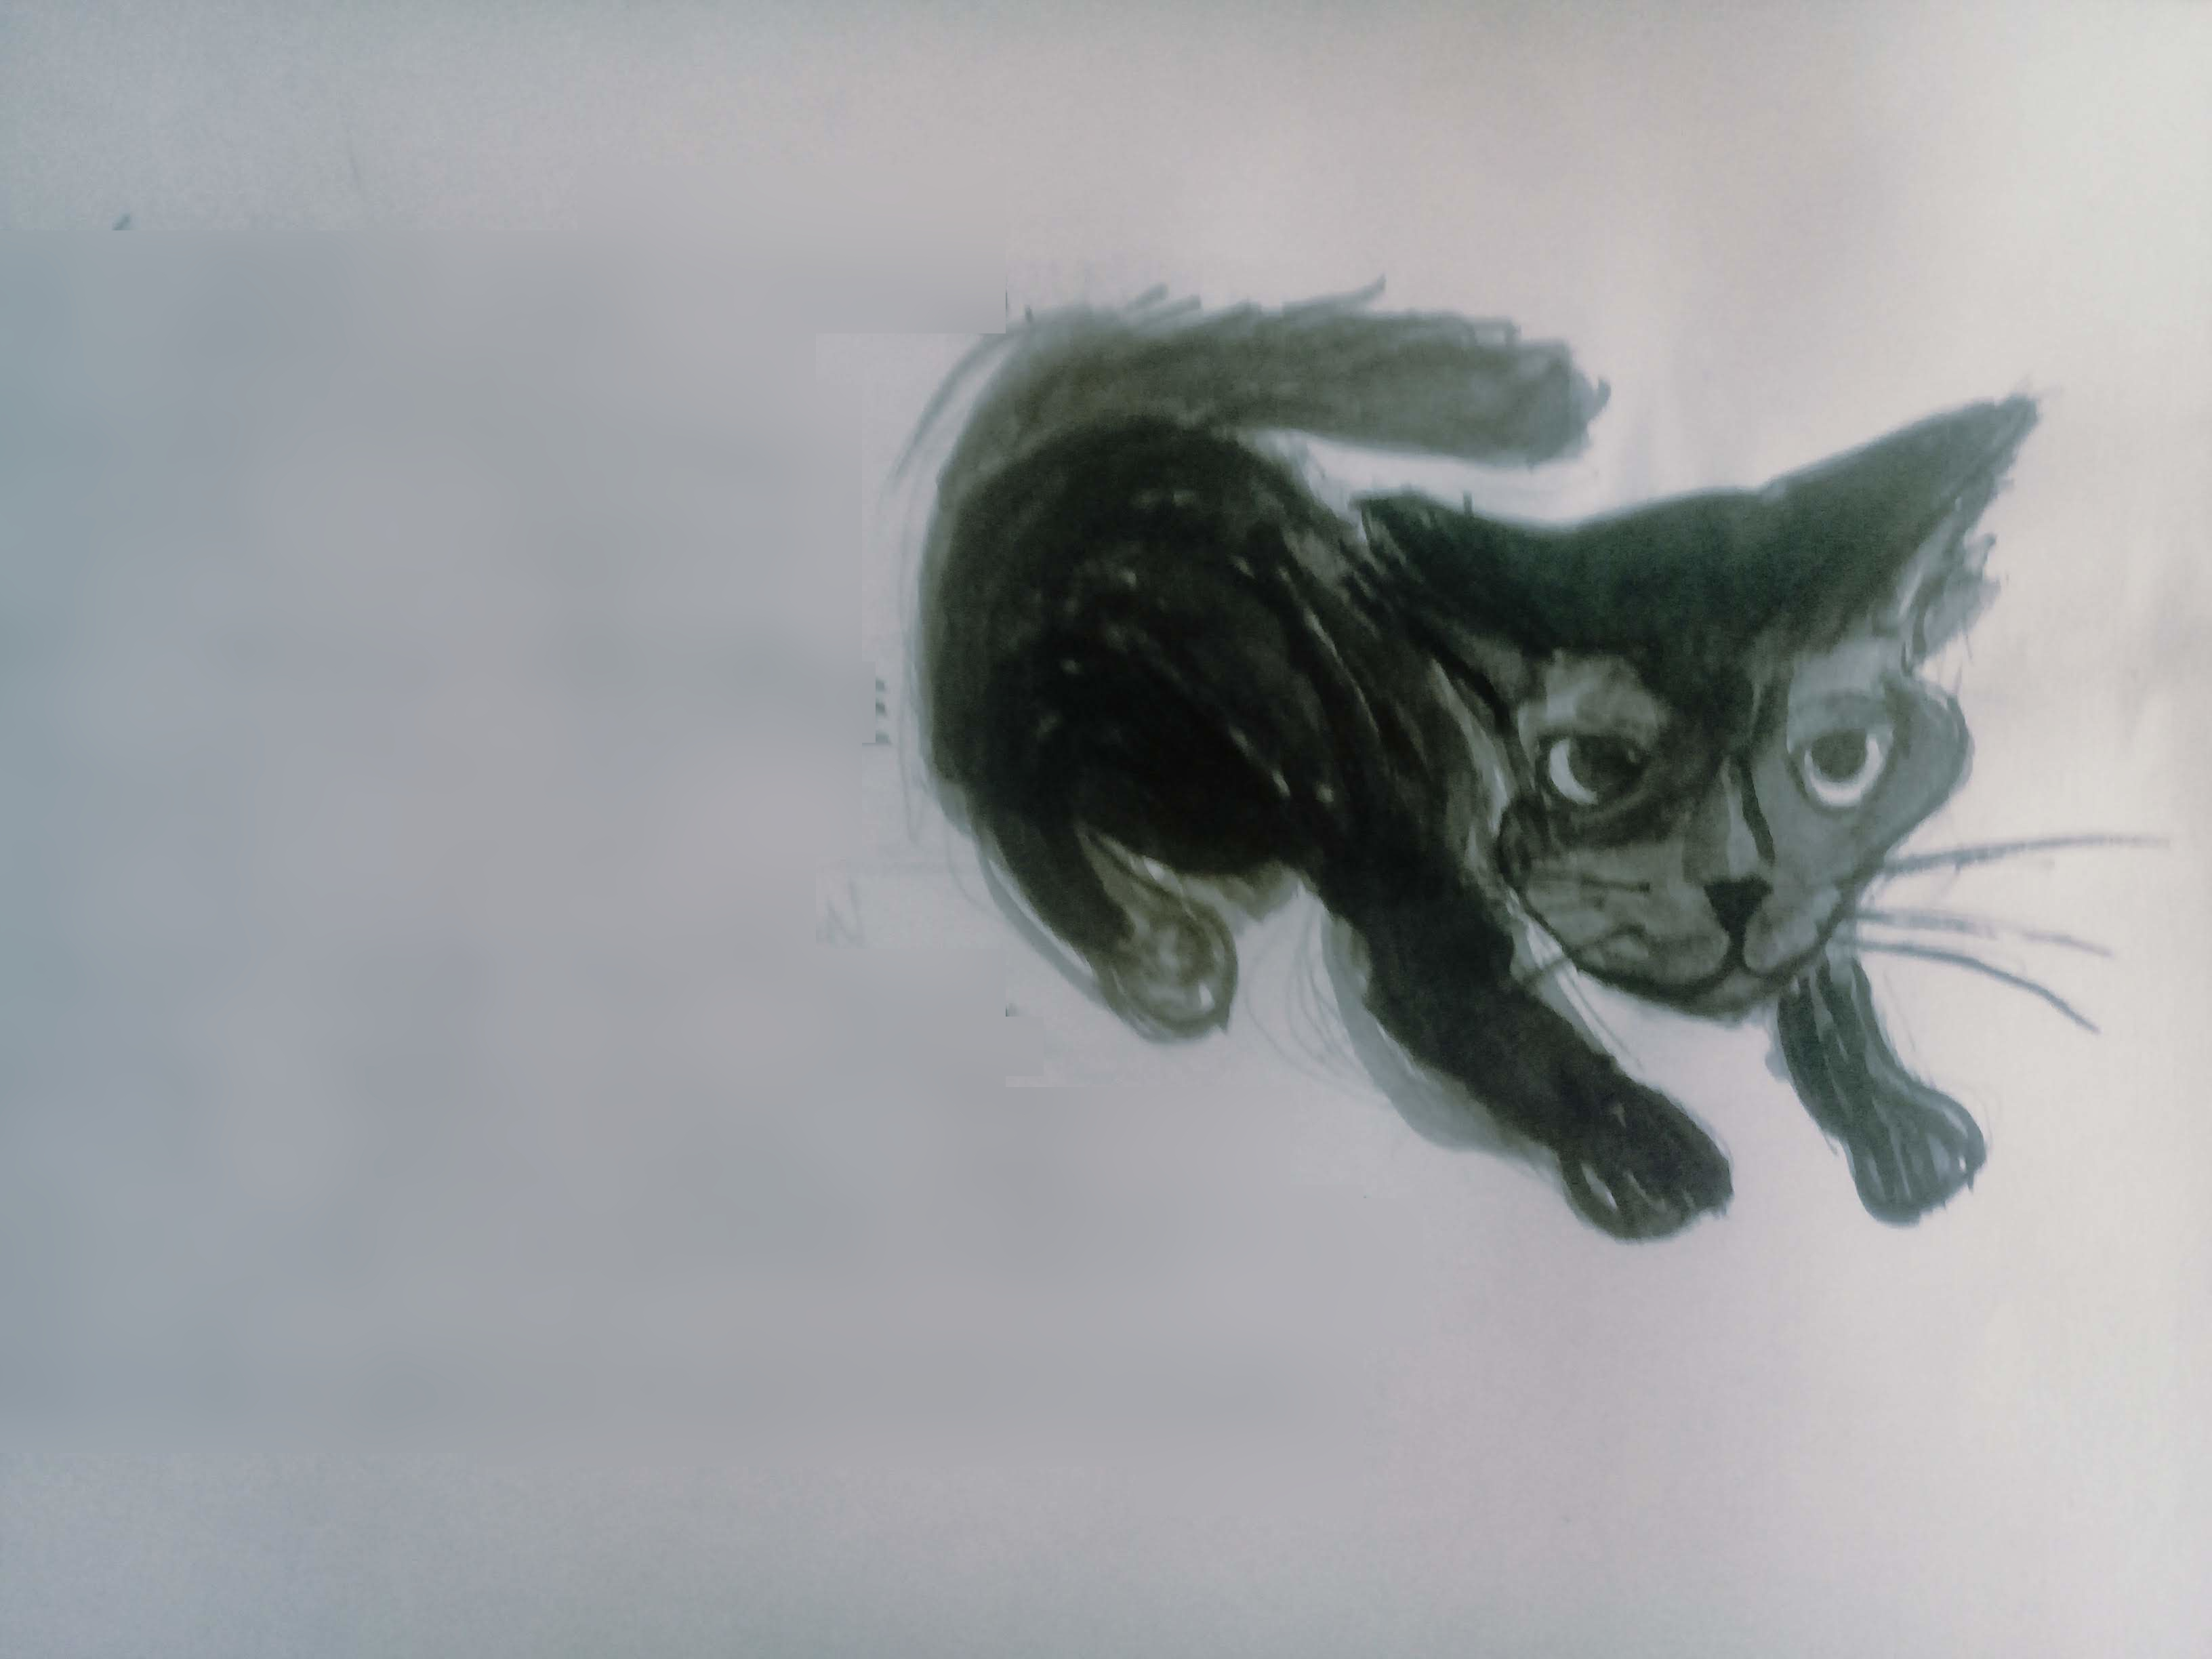
\includegraphics[width=\paperwidth,height=\paperheight,angle=0]{reflexion}};
\end{tikzpicture}
TOMÉ CORAJE Y SEGUÍ TREPANDO. UTILICÉ LA ESQUINA 

QUE FORMAN LAS PAREDES  

Y FINALMENTE ALCANCÉ

TODO LO ALTO 		DEL MURO.

HAY ALLÍ UNA 		ESPECIE 

DE CANTERO Y ME

METÍ DENTRO DE LO QUE

ES  UNA CANALETA. ES DONDE

CORRE  			 EL AGUA QUE MIRO CAER

FASCINADO   LOS DÍAS DE LLUVIA.

DESDE ESE LUGAR  PODÍA VER TODO EL 

PATIO DONDE SOLEMOS JUGAR. MI ESFUERZO RESULTÓ TAN GRANDE QUE NECESITÉ DESCANSAR UN RATO.





\newpage
\begin{tikzpicture}[remember picture, overlay]
	
	\node [inner sep=0pt, minimum width=\paperwidth, minimum height=\paperheight] at (current page.center) {
\includegraphics[width=\paperwidth,height=\paperheight,angle=0]{paper2}};
\end{tikzpicture}

A LOS GATOS NOS GUSTAN LAS SIESTAS EN LAS ALTURAS Y AL CALOR DEL SOL, SOBRE TODO EN INVIERNO.

YA ME HABÍA OLVIDADO DE LAS PALOMAS, HABÍAN VOLADO Y VIENDO UN GATO NEGRO EN LO ALTO DE UN MURO BLANCO, DUDO QUE VOLVERÍAN POR MI CASA POR UN BUEN RATO.

CUANDO ME LEVANTÉ, EXPLORÉ LOS ALREDEDORES PASEANDO POR EL CANTERO. SABÍA QUE AL LADO VIVÍAN DOS PERRITOS BASTANTE CARGOSOS, POR COMO SOLÍAN LADRAR. Y AL FIN LAS VEÍA! ERAN UNA PERRA LABRADOR NEGRA Y UNA CANICHE BLANCA. PASEABAN SIN CORREA, SEGUIDAS POR UN VIEJO DE CAMINAR TORPE Y DESCUIDADO. LAS PERRITAS SE PUSIERON A HACER SUS COSAS  EN LA VEREDA Y EL SEÑOR NI AMAGÓ PARA LIMPIARLA.



\newpage
\begin{tikzpicture}[remember picture, overlay]
	
	\node [inner sep=0pt, minimum width=\paperwidth, minimum height=\paperheight] at (current page.center) {
\includegraphics[width=\paperwidth,height=\paperheight,angle=0]{paper2}};
	\node[xshift=.35\textwidth] at (current page.center){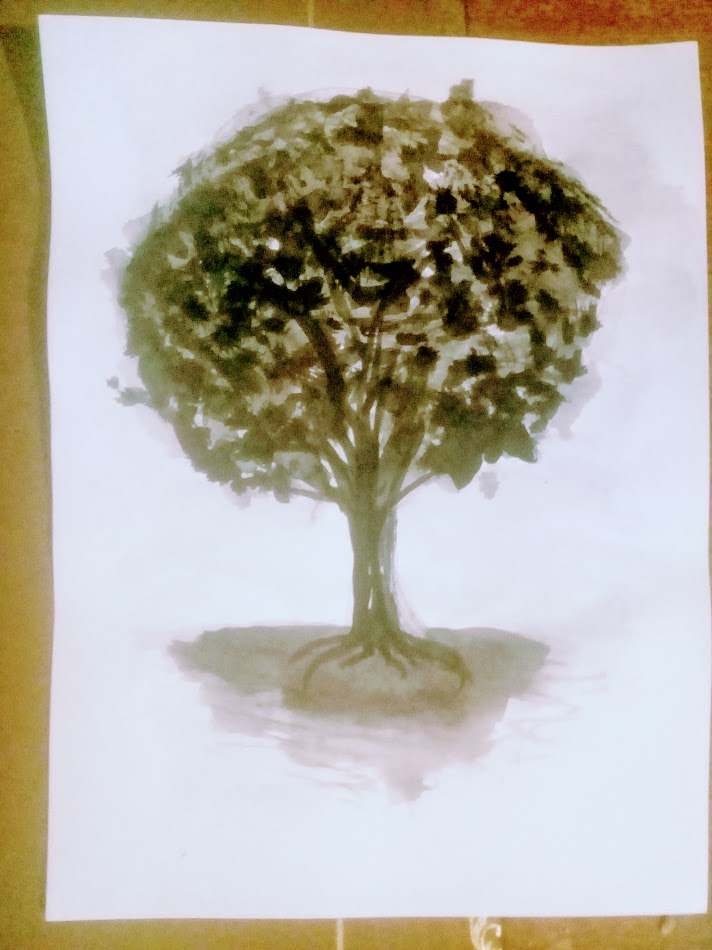
\includegraphics[width=.5\textwidth,trim=1.9cm 2cm 1.5cm 1.6cm,clip]{arbol_tilo}};
\end{tikzpicture}
ESPERÉ UN RATO, NO PODRÍA BAJAR CON 

ESAS DOS PERRITAS 	SUELTAS. Y PARA PODER 

DESCENDER, 		NECESITABA ALGO ENTRE 

EL		
ALTO MURO Y EL PISO. 

PENSÉ EN LOS ÁRBOLES DE TILO QUE 

ESTÁN 		JUNTO A LA CASA. 		SON MUY 

LINDOS, DE COPAS REPLETAS DE HOJAS EN 

PRIMAVERA, Y  QUE CAEN, JUNTO A SEMILLAS 

DURANTE EL OTOÑO. MUCHAS DE ELLAS TERMINAN

EN NUESTRO PATIO Y SON BUENOS JUGUETES.

PERO SUFICIENTE CON LOS JUEGOS. 
SIEMPRE ME

DICEN QUE PAREZCO UNA PEQUEÑA PANTERA 
NEGRA$\ldots$ 

ERA HORA DE DEMOSTRARLO. 






\newpage
\begin{tikzpicture}[remember picture, overlay]
	
	\node [inner sep=0pt, minimum width=\paperwidth, minimum height=\paperheight] at (current page.center) {
\includegraphics[width=\paperwidth,height=\paperheight,angle=0]{paper3}};
\end{tikzpicture}	
DURANTE MI SIESTA YA HABÍA PENSADO EN EL SALTO. A MENUDO PIENSO EN MIS PROEZAS FELINAS A LA HORA DE DORMIR, ASÍ ME DUERMO CON UNA SONRISA.

PERO AHORA, BIEN DESPIERTO, NO IBA A FALLAR NINGÚN CÁLCULO. TODO MI ENTRENAMIENTO EN EL PATIO, TREPANDO EN LA BIBLIOTECA, SOBRE EL PIANO, SOBRE LA SILLA ALTA$\ldots$ TODO IBA A SERVIRME EN MI CAÍDA CON ESTILO SOBRE LA RAMA DEL ÁRBOL DE TILO.  



\newpage
\begin{tikzpicture}[remember picture, overlay]
	
	\node [inner sep=0pt, minimum width=\paperwidth, minimum height=\paperheight] at (current page.center) {
\includegraphics[width=\paperwidth,height=\paperheight,angle=0]{paper3}};
	\node[xshift=0cm,yshift=4cm] at (current page.center){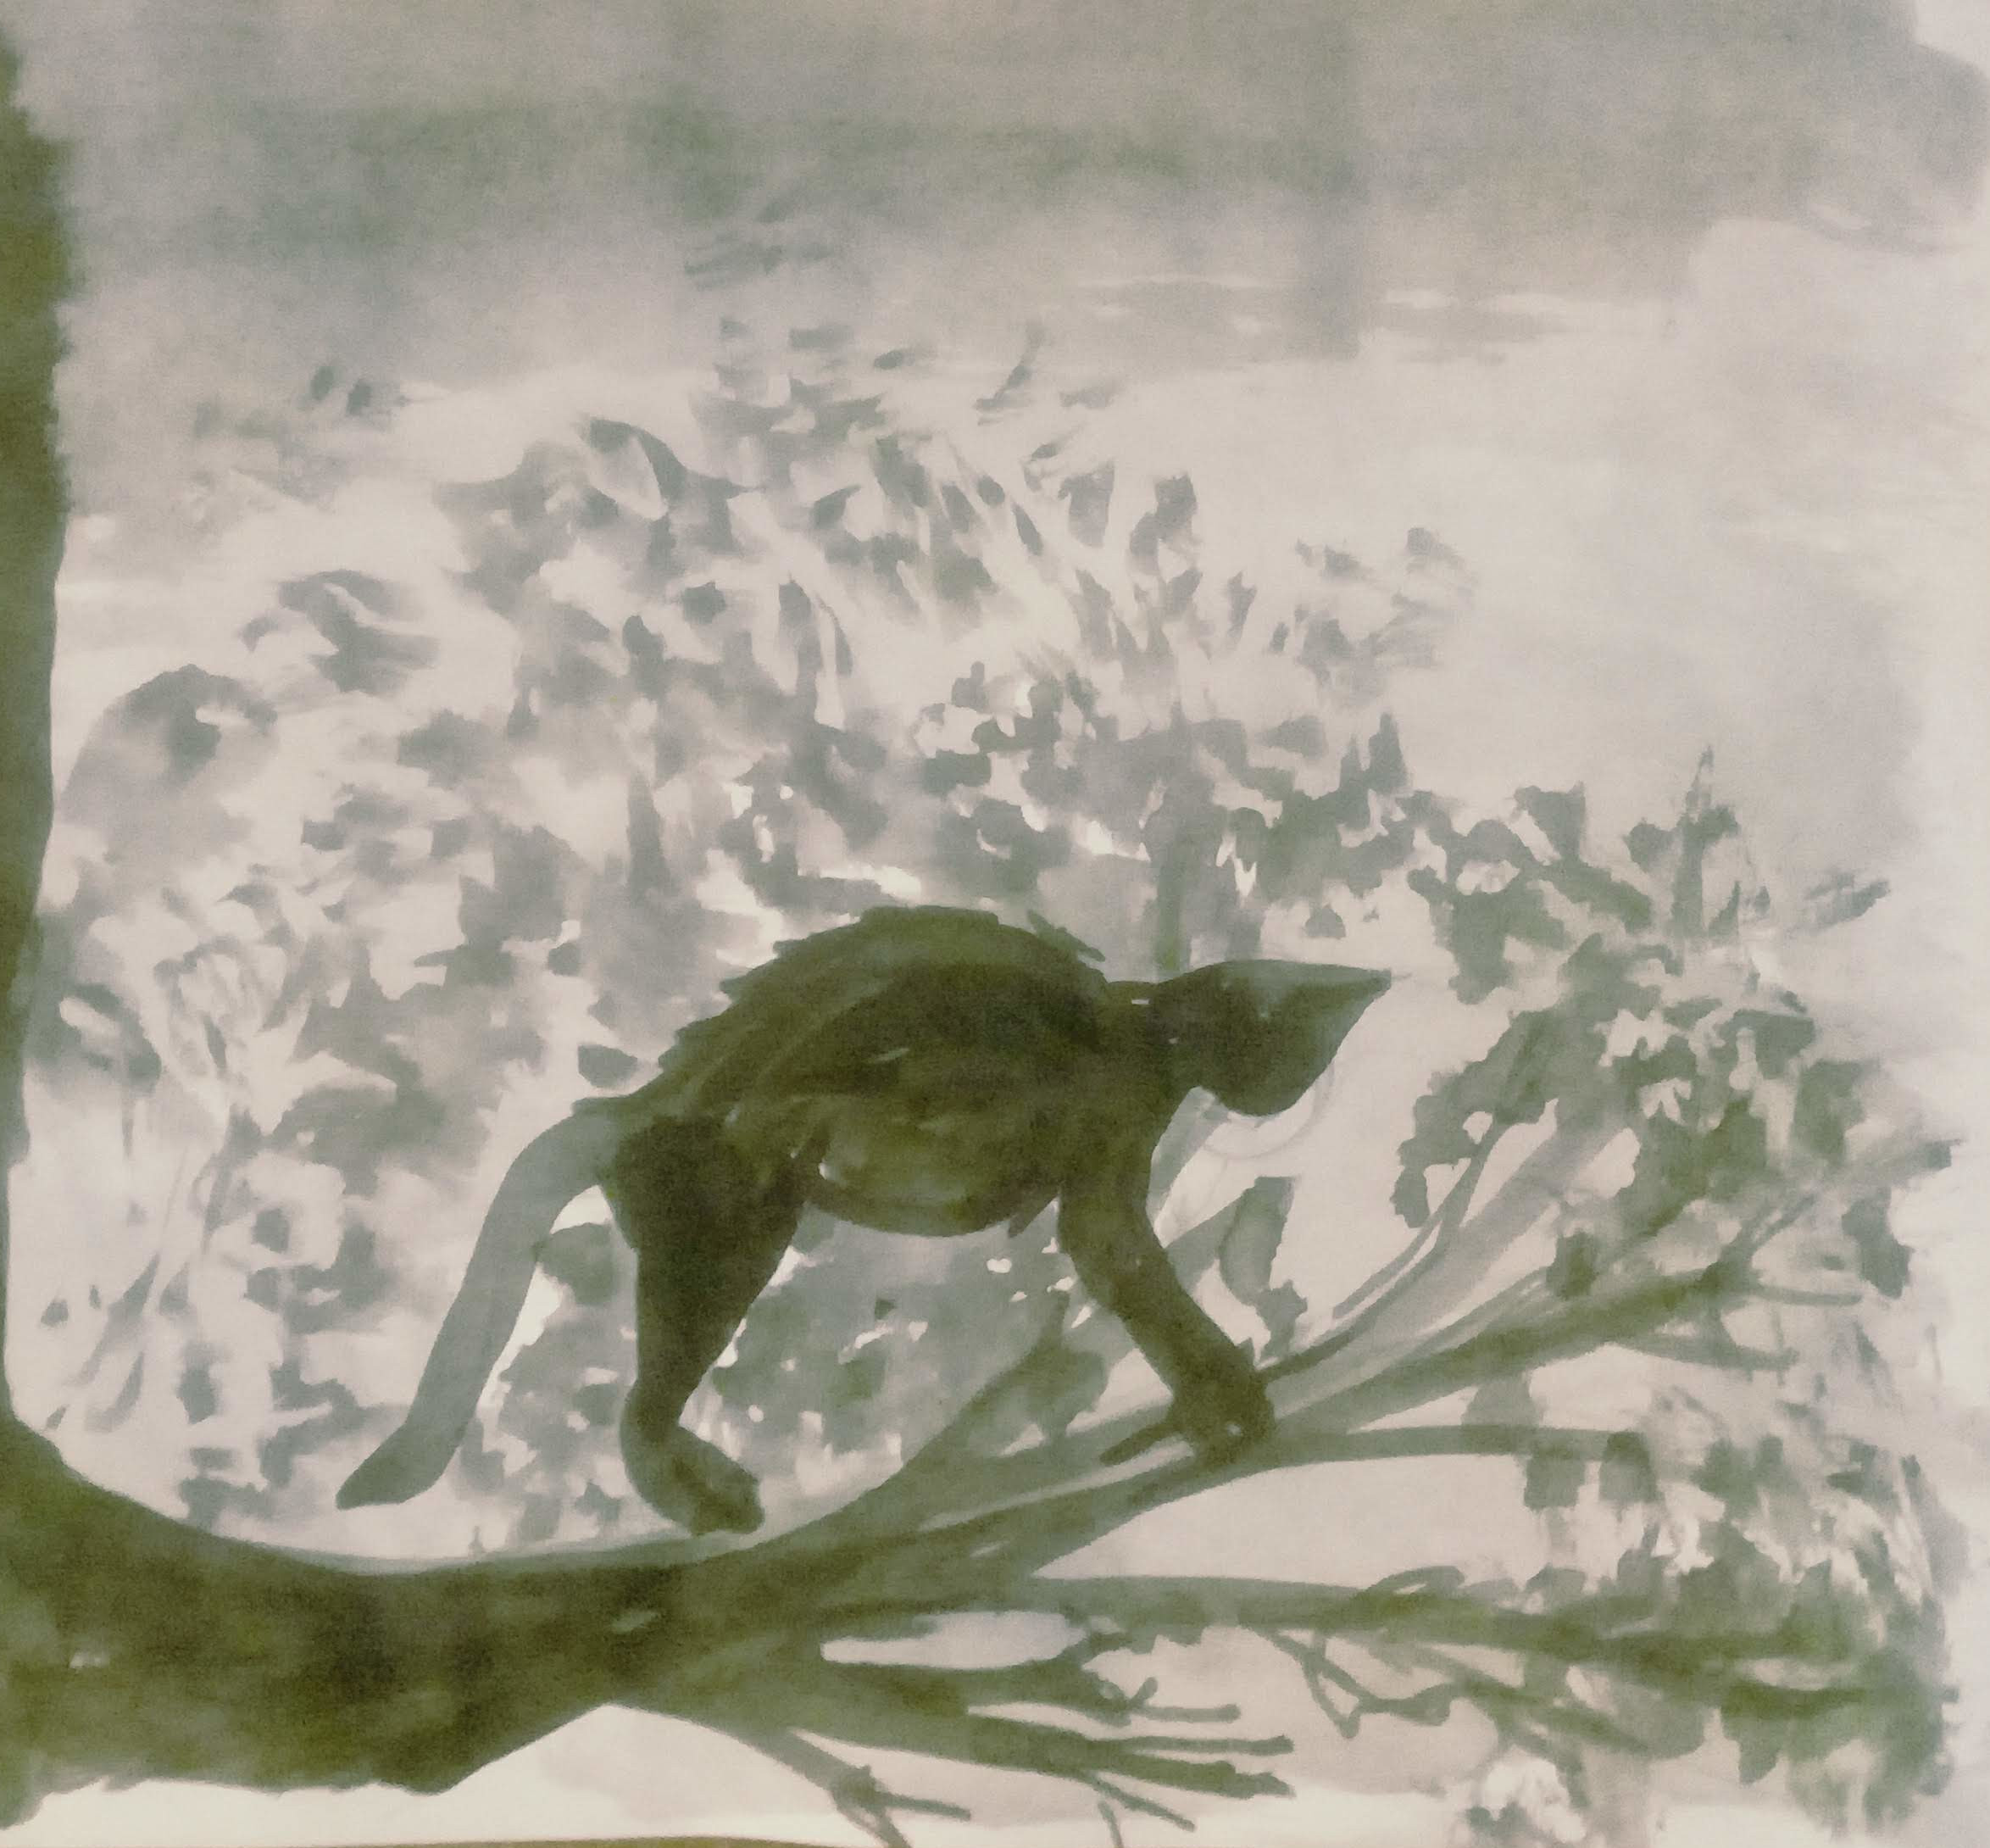
\includegraphics[width=.8\textwidth,trim=1.9cm 2cm 1.5cm 1.6cm,clip]{arriba_arbol}};
\end{tikzpicture}

\vspace{.7\textheight}
Y ASÍ FUE, UNA MANIOBRA LIMPIA Y DISTINGUIDA, SÉ QUIENES ESTARÍAN ORGULLOSOS DE MÍ. 





\newpage
\begin{tikzpicture}[remember picture, overlay]
	
	\node [inner sep=0pt, minimum width=\paperwidth, minimum height=\paperheight] at (current page.center) {
\includegraphics[width=\paperwidth,height=\paperheight,angle=0]{paper3}};
\end{tikzpicture}	
% 		\node[xshift=7cm,yshift=3cm] at (current page.center){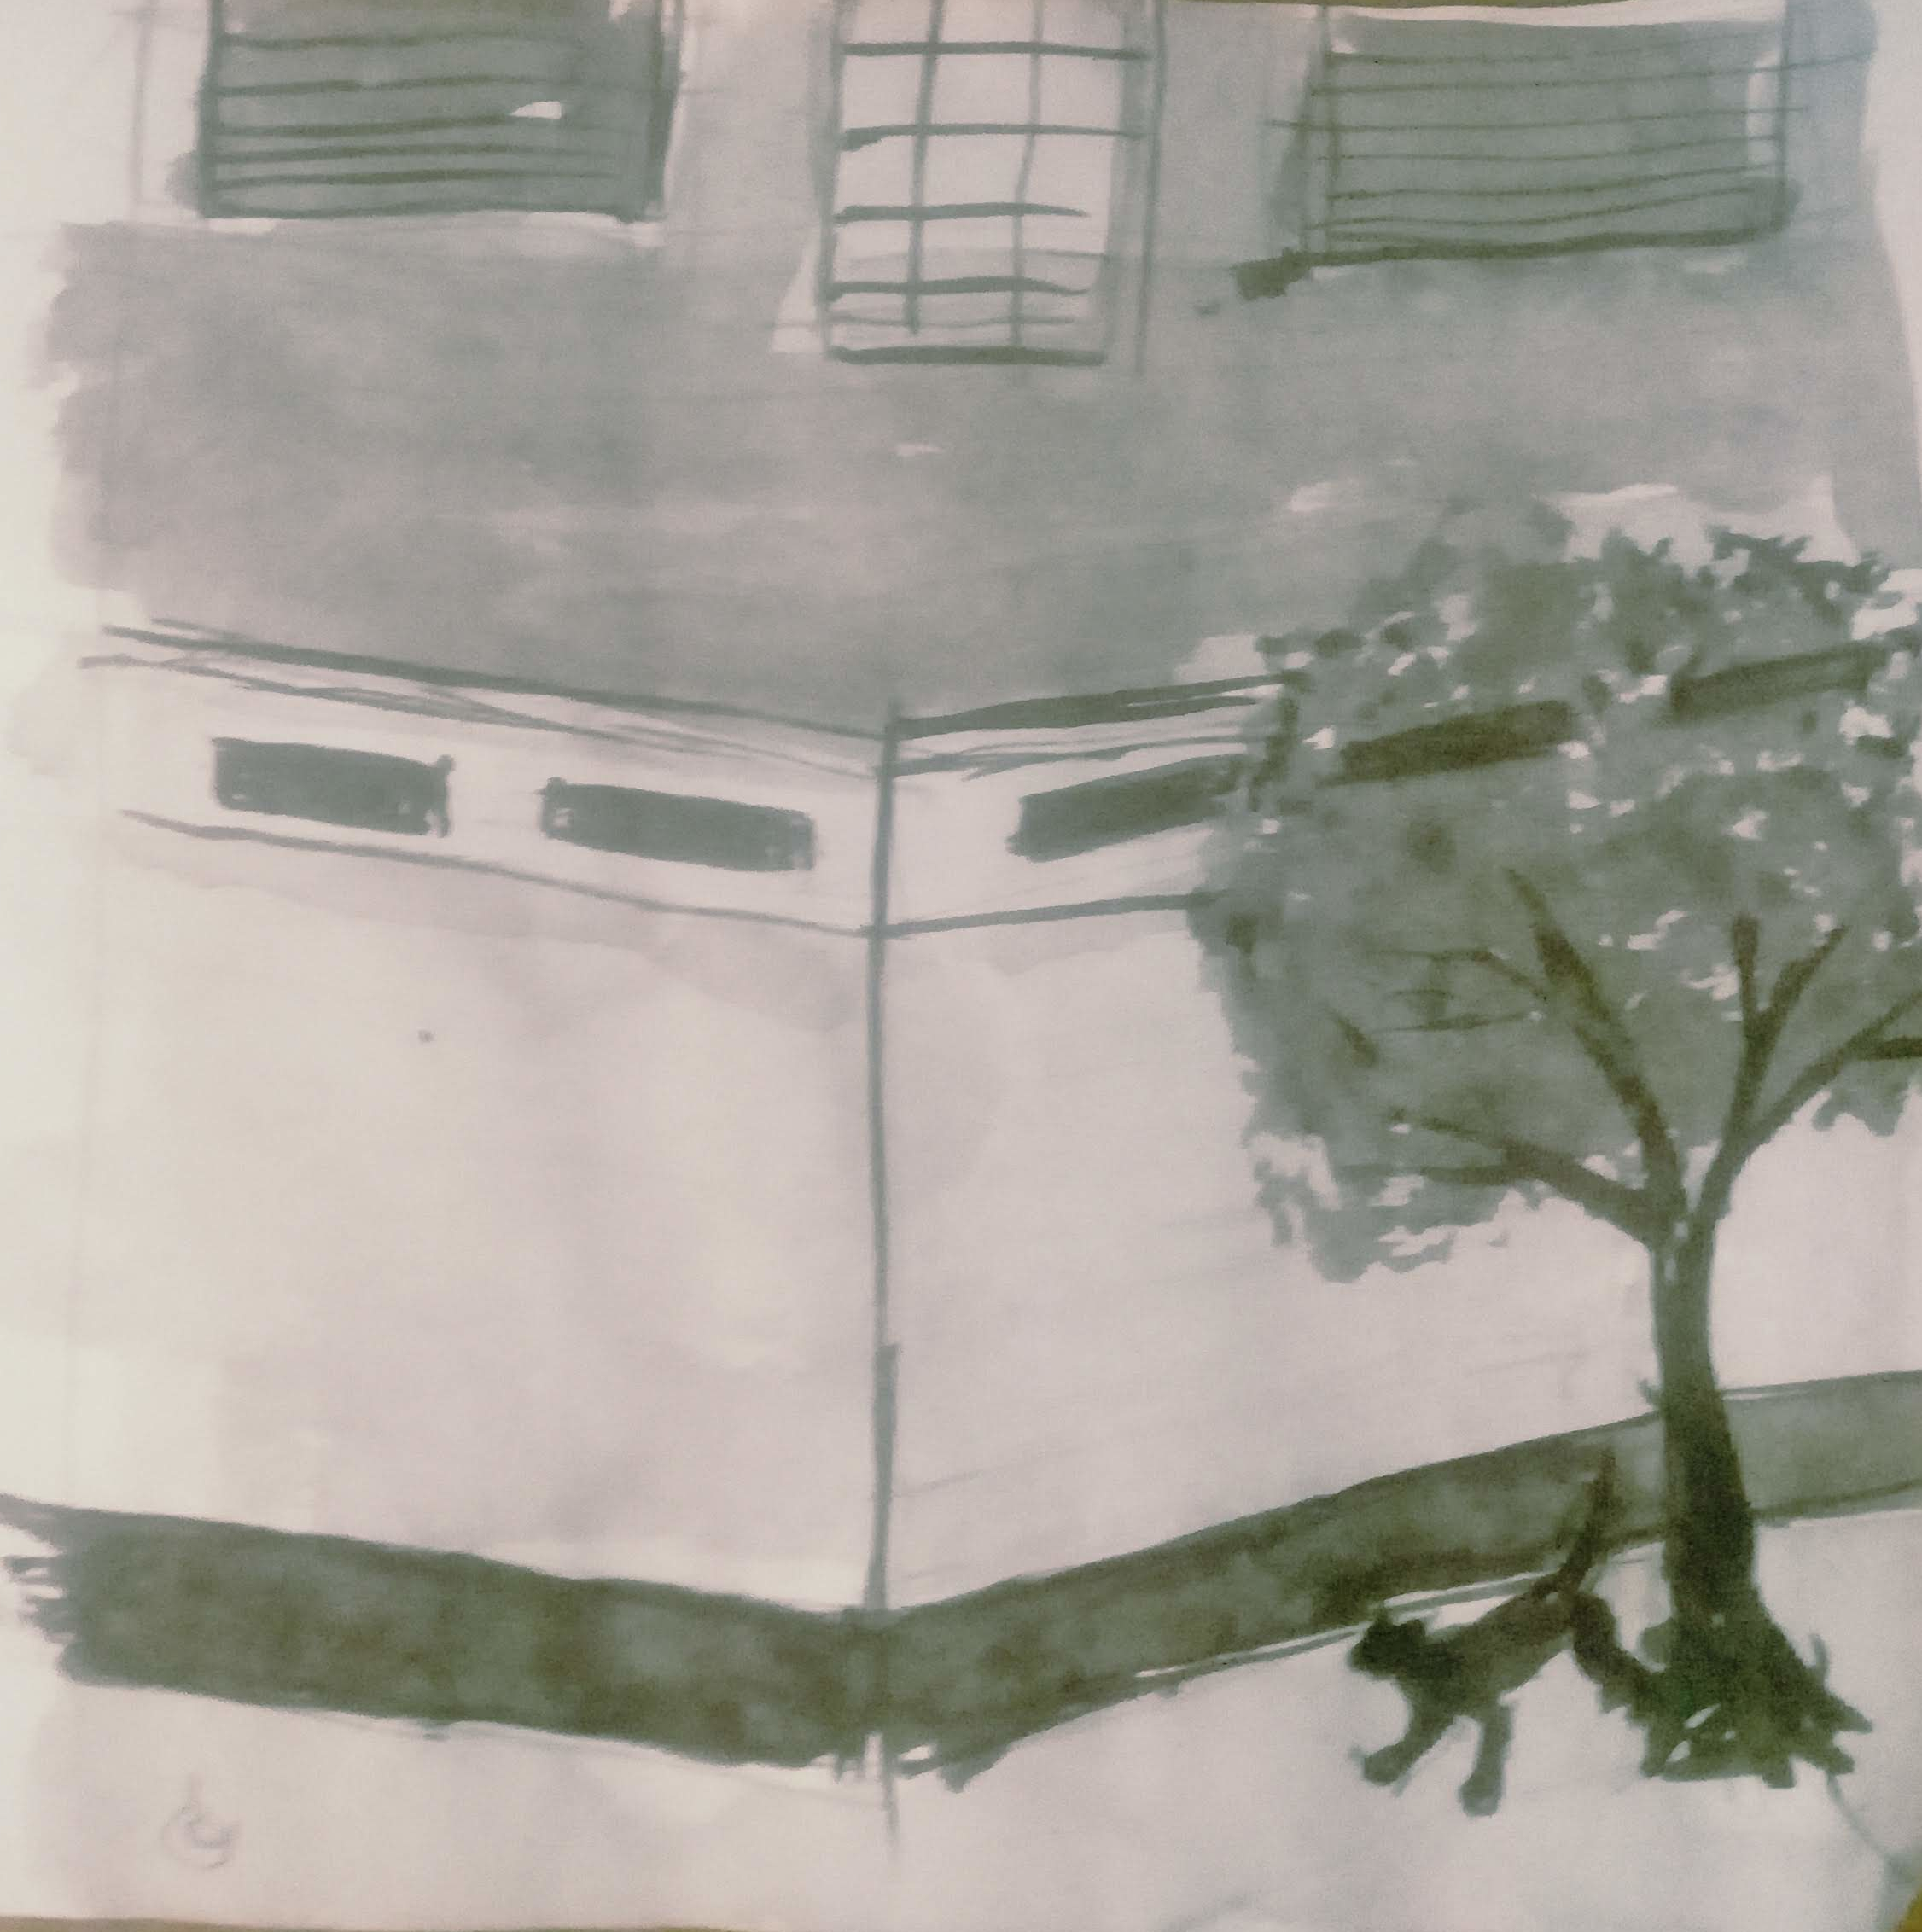
\includegraphics[width=.4\textwidth,trim=1cm 0cm 1.cm 0cm,clip]{vereda1}};
% 		\node[text width=24cm,yshift=0cm] at (current page.center){
	YA CAMINANDO POR LA VEREDA, DESDE AFUERA, LA CASA SE VEÍA
	MÁS GRANDE. VI ACERCARSE UN PERRO Y VOLVÍ A TREPARME AL ÁRBOL SIN PROBLEMAS.
	
	
	\begin{wrapfigure}{r}{.45\textwidth}
		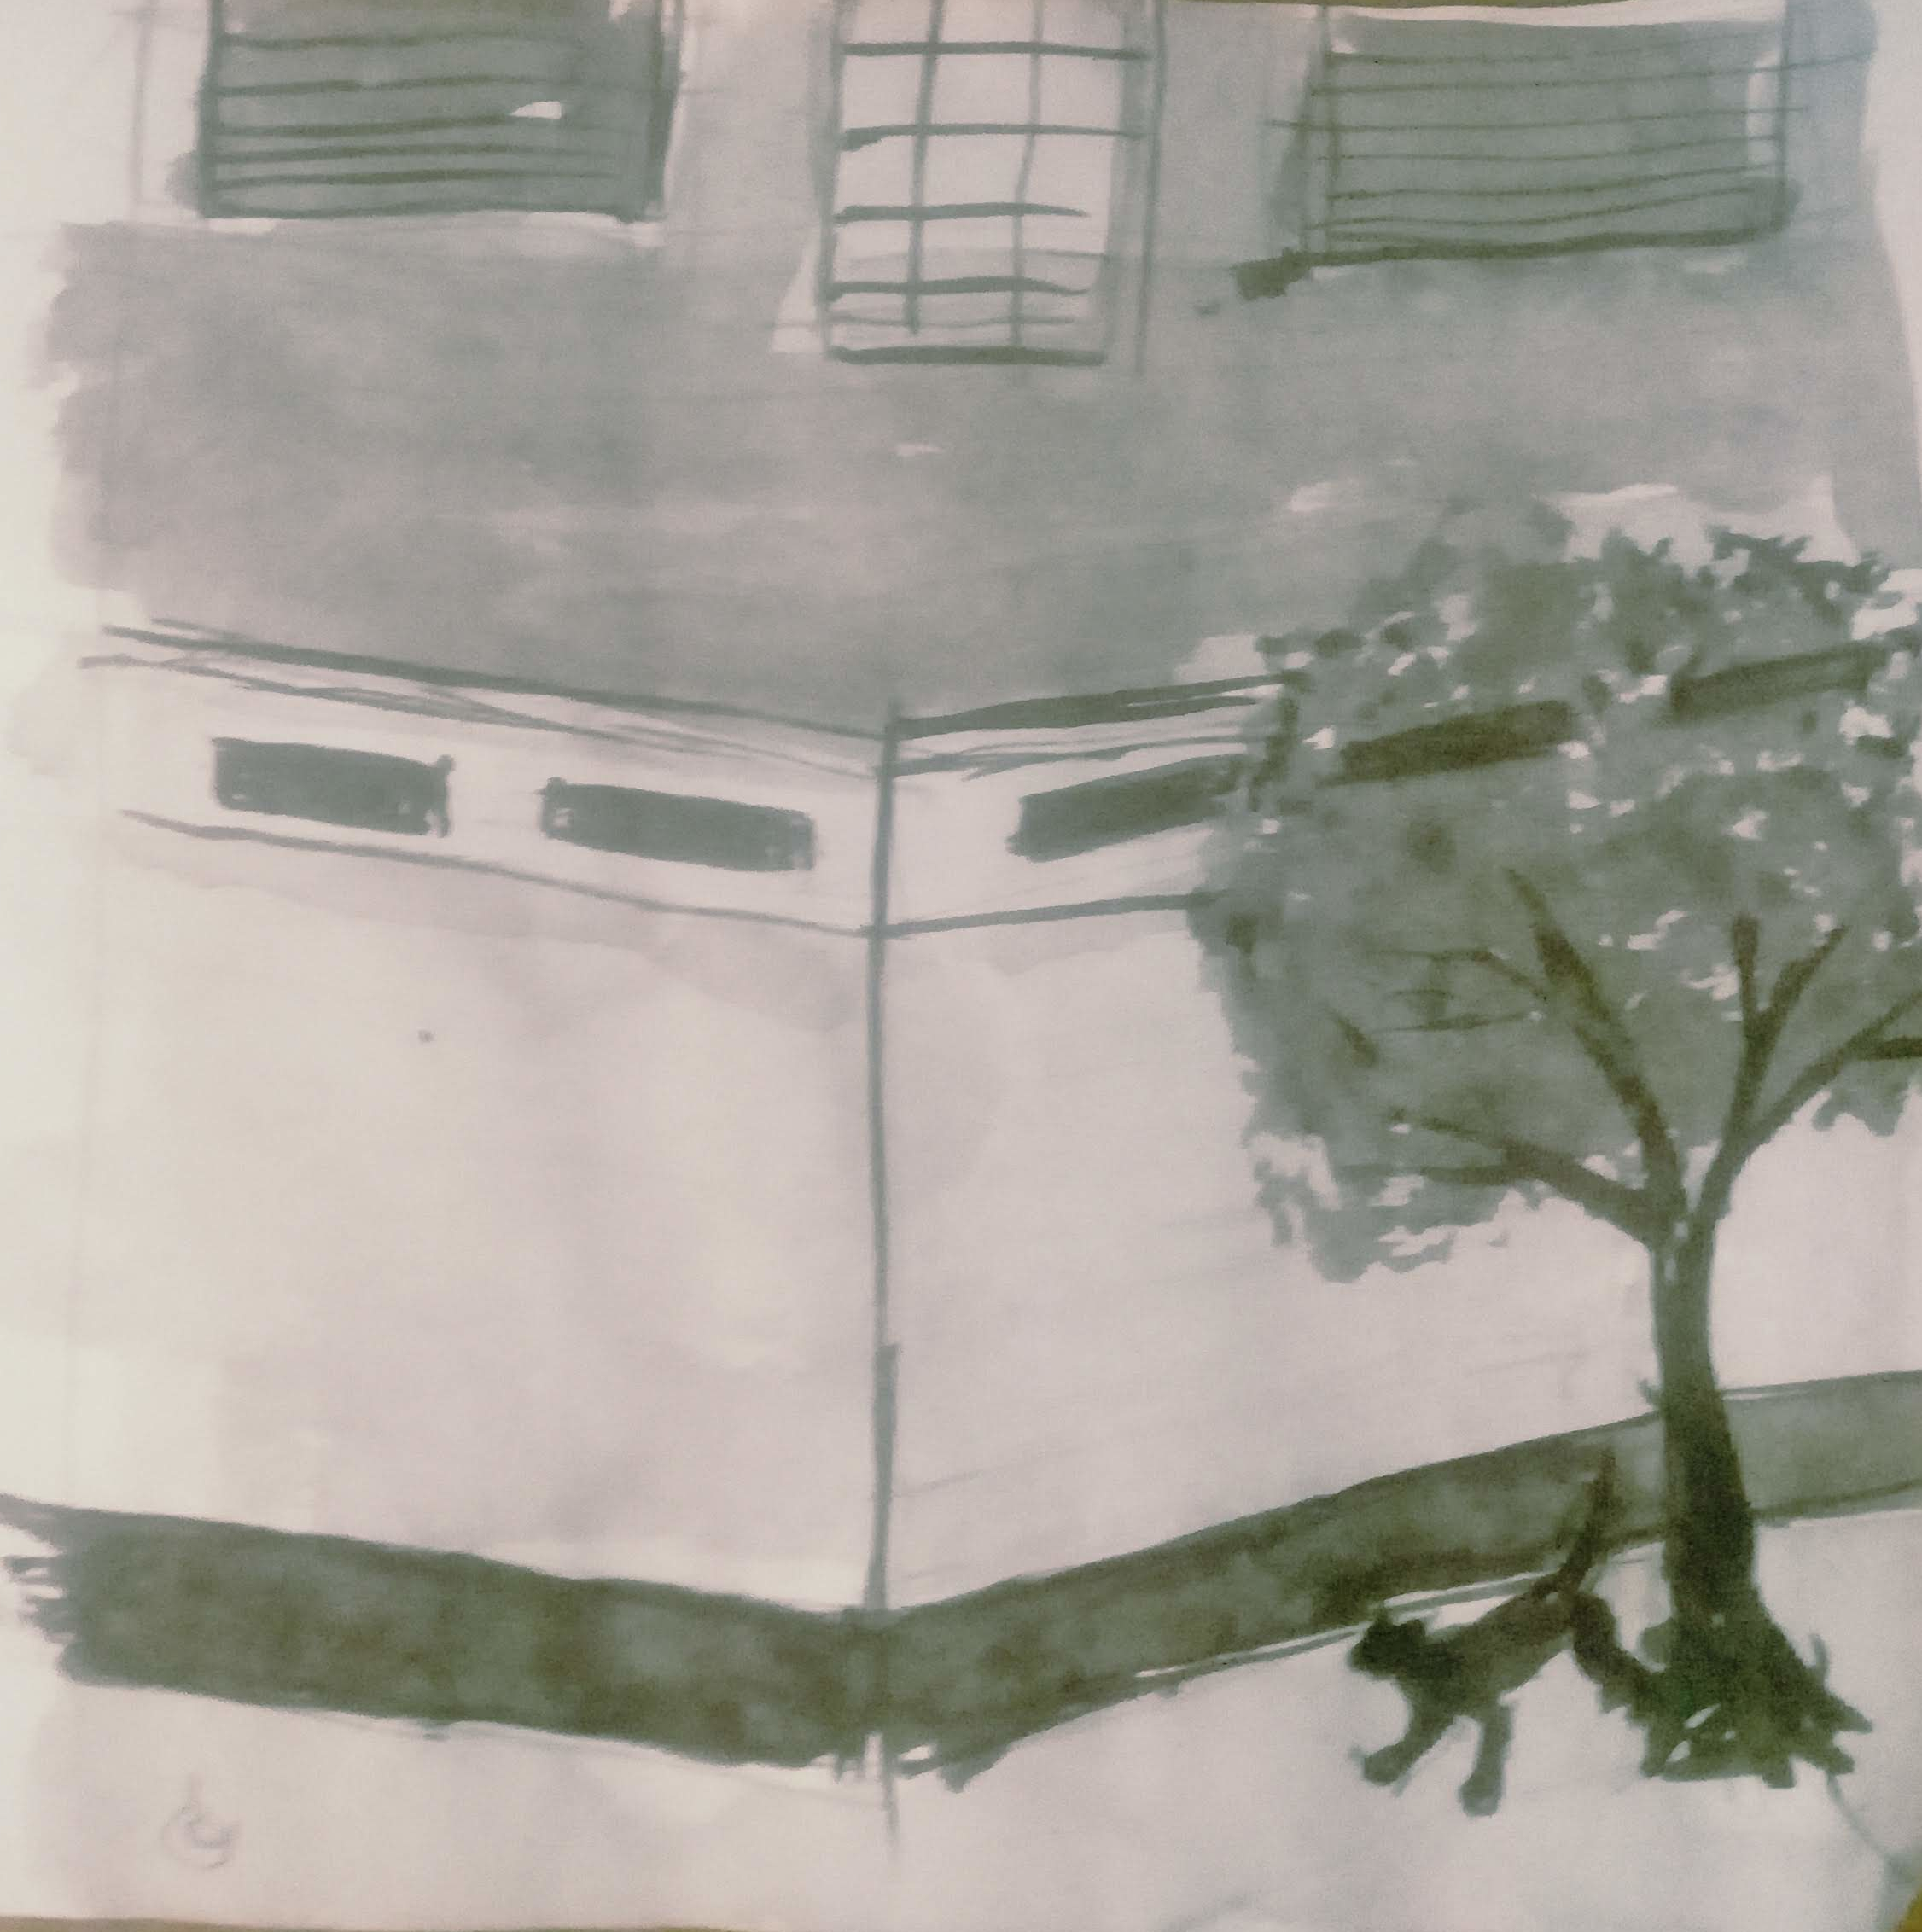
\includegraphics[width=.4\textwidth,trim=1cm 0cm 1.cm 0cm,clip]{vereda1}
	\end{wrapfigure}
	AHORA QUE ME HABÍA OLVIDADO  DE 
	
	LAS PALOMAS, DI UNA VUELTA A LA PEQUEÑA MANZANA QUE CONTIENE A MI CASA. YA HABÍA VISTO UN POCO LA CALLE CUANDO  ME HABÍAN LLEVADO A VACUNAR.  
	PERO, ¿QUÉ DIRECCIÓN TOMAR? DECIDÍ IR HACIA DONDE VIERA PERSONAS.
	
	
	\newpage
	\begin{tikzpicture}[remember picture, overlay]
		\node [inner sep=0pt, minimum width=\paperwidth, minimum height=\paperheight] at (current page.center) {
\includegraphics[width=\paperwidth,height=\paperheight,angle=0]{paper4}};
	\end{tikzpicture}	
	PUES PODÍA SER INTERESANTE APRENDER ALGO NUEVO. FUI AVANZANDO DE POCO ESCONDIÉNDOME PRIMERO EN UN CANTERO, LUEGO DETRÁS DE UNAS PALMERAS.
	
	IBA A TENER QUE CRUZAR LA CALLE. ES UNA SENSACIÓN DISTINTA,  PUES  LA SUPERFICIE NO ES LA MISMA QUE LA VEREDA Y HAY UNA BAJADITA, QUE LLAMAN CORDÓN.
	
	A MENUDO, HAY ASFALTO, QUE ES UNA SUPERFICIE LISA Y UN POCO RUGOSA A LA VEZ. 
	
	
	LOS ADOQUINES, EN CAMBIO, SON COMO PIEDRAS TODAS DEL MISMO TAMAÑO, ORDENADAS REGULARMENTE. SE VEN MUY DUROS Y LISOS, AUNQUE LOS AUTOS CUANDO PASAN HACEN MUCHO RUIDO PORQUE LES DAN COMO GOLPECITOS.  	  
	
	
	EN OCASIONES, SE CONSERVAN DESDE LA ÉPOCA DE CUANDO MI PAPÁ ERA CHIQUITO.
	%};


\newpage
\begin{tikzpicture}[remember picture, overlay]
	\node [inner sep=0pt, minimum width=\paperwidth, minimum height=\paperheight] at (current page.center) {
\includegraphics[width=\paperwidth,height=\paperheight,angle=0]{paper4}};
\end{tikzpicture}
\begin{wrapfigure}{r}{.4\textwidth}
	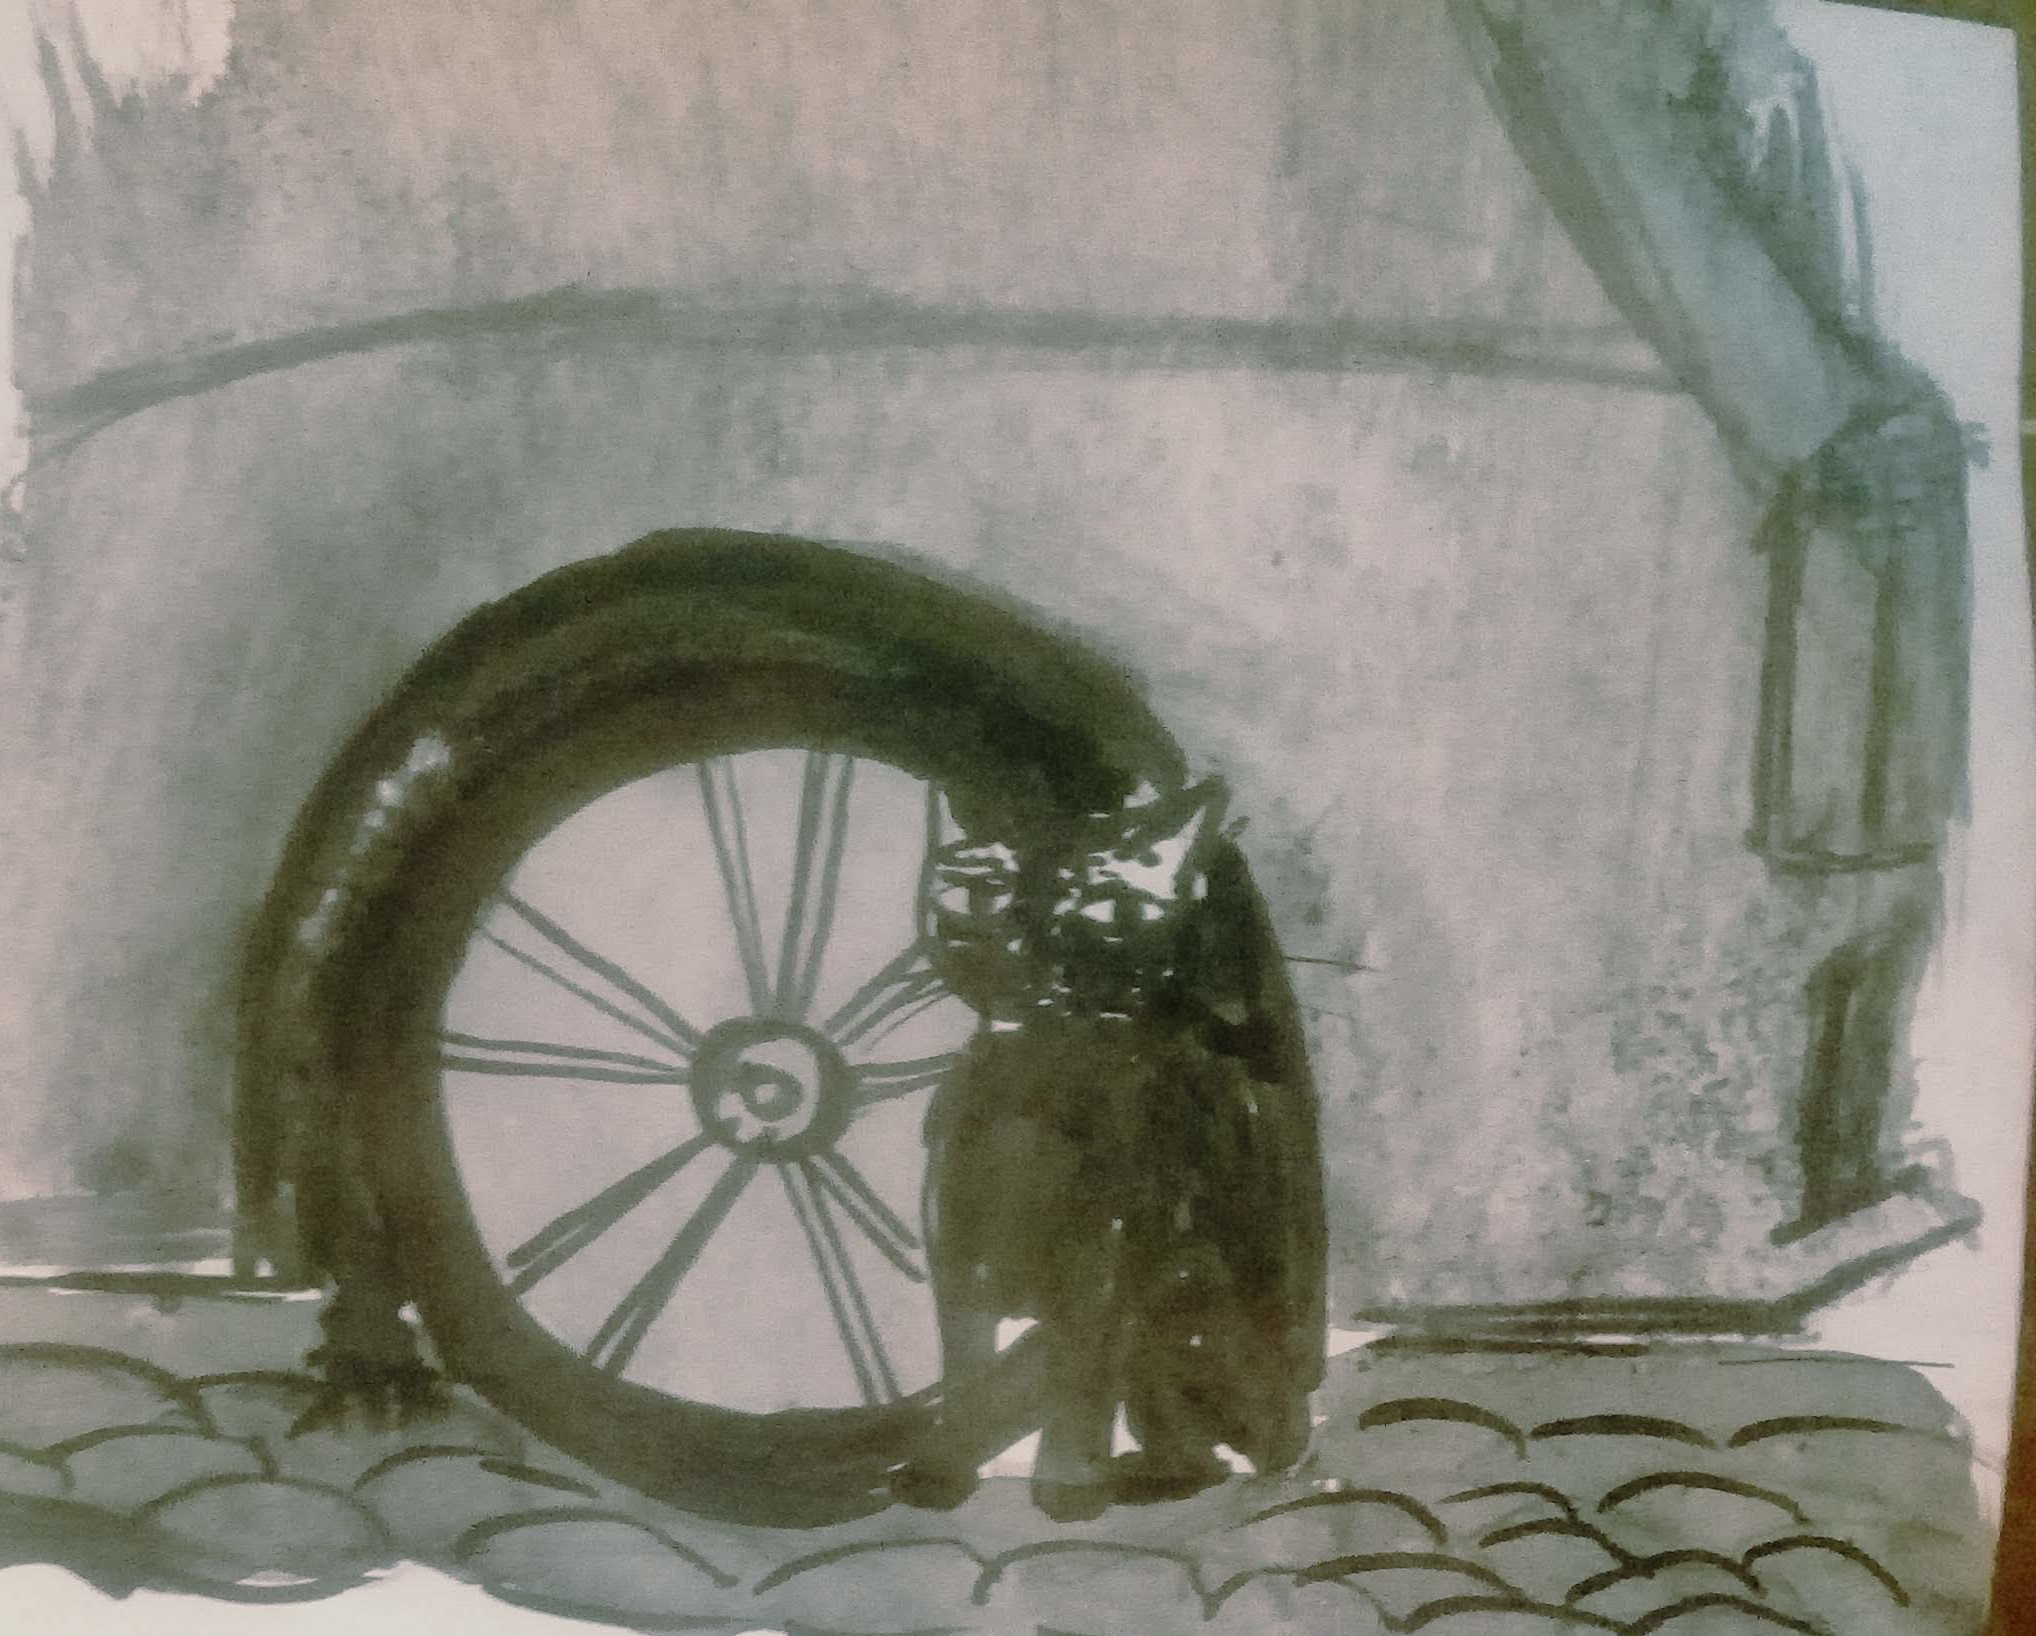
\includegraphics[width=.4\textwidth,trim=1cm 0cm 1.cm 0cm,clip]{rueda_auto}
\end{wrapfigure}
ANTES DE IR SOBRE LA CALLE, ME DETUVE UNOS INSTANTES AL COSTADO DE UNA RUEDA DE AUTO.
ATRAVESÉ LA CALLE DE ADOQUINES MIRANDO BIEN QUE NO HUBIERA NINGÚN AUTO EN MOVIMIENTO.  NI BIEN LLEGUÉ A LA OTRA VEREDA, PERCIBÍ UN AROMA DELICIOSO. YA LO HABÍA SENTIDO ANTES,	 HACE UNOS MESES, CREO QUE 
SE TRATABA DE COMIDA CHINA: CHAW FAN Y BUÑUELOS DE POLLO!

\newpage

\begin{tikzpicture}[remember picture, overlay]
	
	\node [inner sep=0pt, minimum width=\paperwidth, minimum height=\paperheight] at (current page.center) {
\includegraphics[width=\paperwidth,height=\paperheight,angle=0]{paper5}};
\end{tikzpicture}
\begin{wrapfigure}{r}{.53\textwidth}
	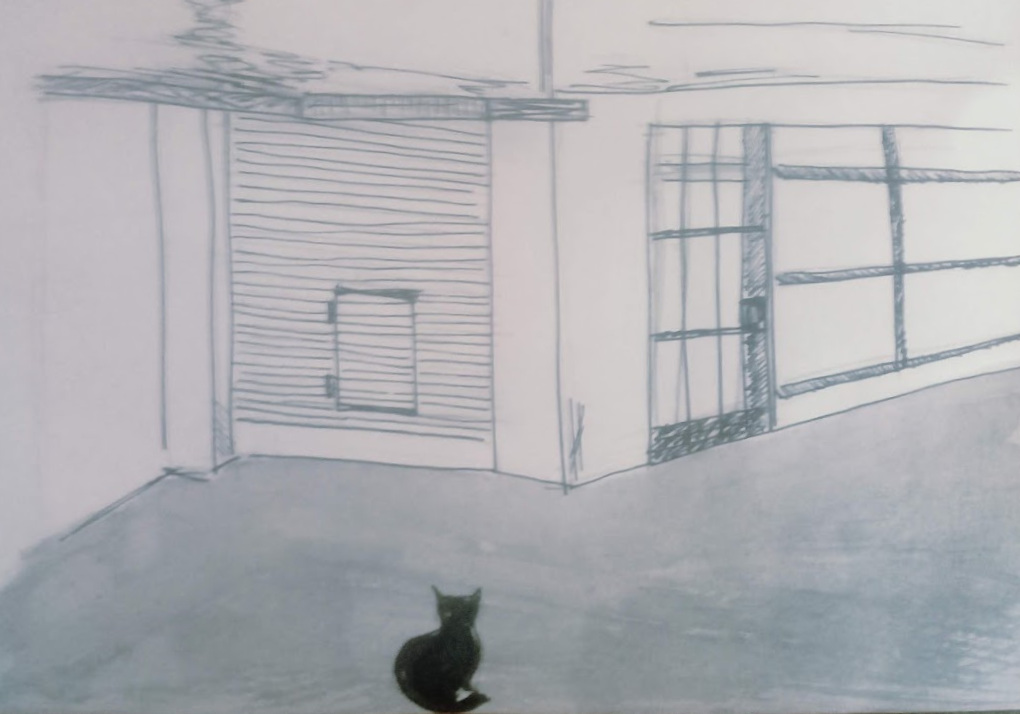
\includegraphics[width=.5\textwidth,trim=0cm 0cm 0.cm 0cm,clip]{comida_china}
\end{wrapfigure}
PERO NO VEÍA NADA MÁS QUE UNA PERSIANA DE METAL BAJA Y AL LADO UNA PUERTA CERRADA. AGUCÉ MI OÍDO FELINO Y ESCUCHÉ MOVIMIENTO DE PERSONAS AL INTERIOR.  DE PRONTO, 
SENTÍ UN AUTO ACERCARSE Y ME DÍ VUELTA. SE TRATABA DE UN AUTO CON LUCES PARPADEANTES AZULES Y SE DETUVO
JUSTO A METROS DE DONDE YO ESTABA. DE UN SALTO ME PUSE A UNA BUENA DISTANCIA A OBSERVAR. 
DESCENDIÓ UN SEÑOR QUE VESTÍA UN UNIFORME AZUL OSCURO, Y RÁPIDAMENTE SE ACERCÓ A LA PERSIANA.


\newpage

\begin{tikzpicture}[remember picture, overlay] 
	
	\node [inner sep=0pt, minimum width=\paperwidth, minimum height=\paperheight] at (current page.center) {
\includegraphics[width=\paperwidth,height=\paperheight,angle=0]{paper6}};
\end{tikzpicture}


EL UNIFORMADO GOLPEÓ RÁPIDO TRES VECES CON LA MITAD DE SU DEDO ÍNDICE  EN LA PERSIANA.
DE PRONTO, UNA PEQUEÑA PUERTA SE ABRIÓ Y UN BRAZO ASOMÓ CON	  LO QUE IMAGINÉ ERA UN
\begin{wrapfigure}{r}{.5\textwidth}
	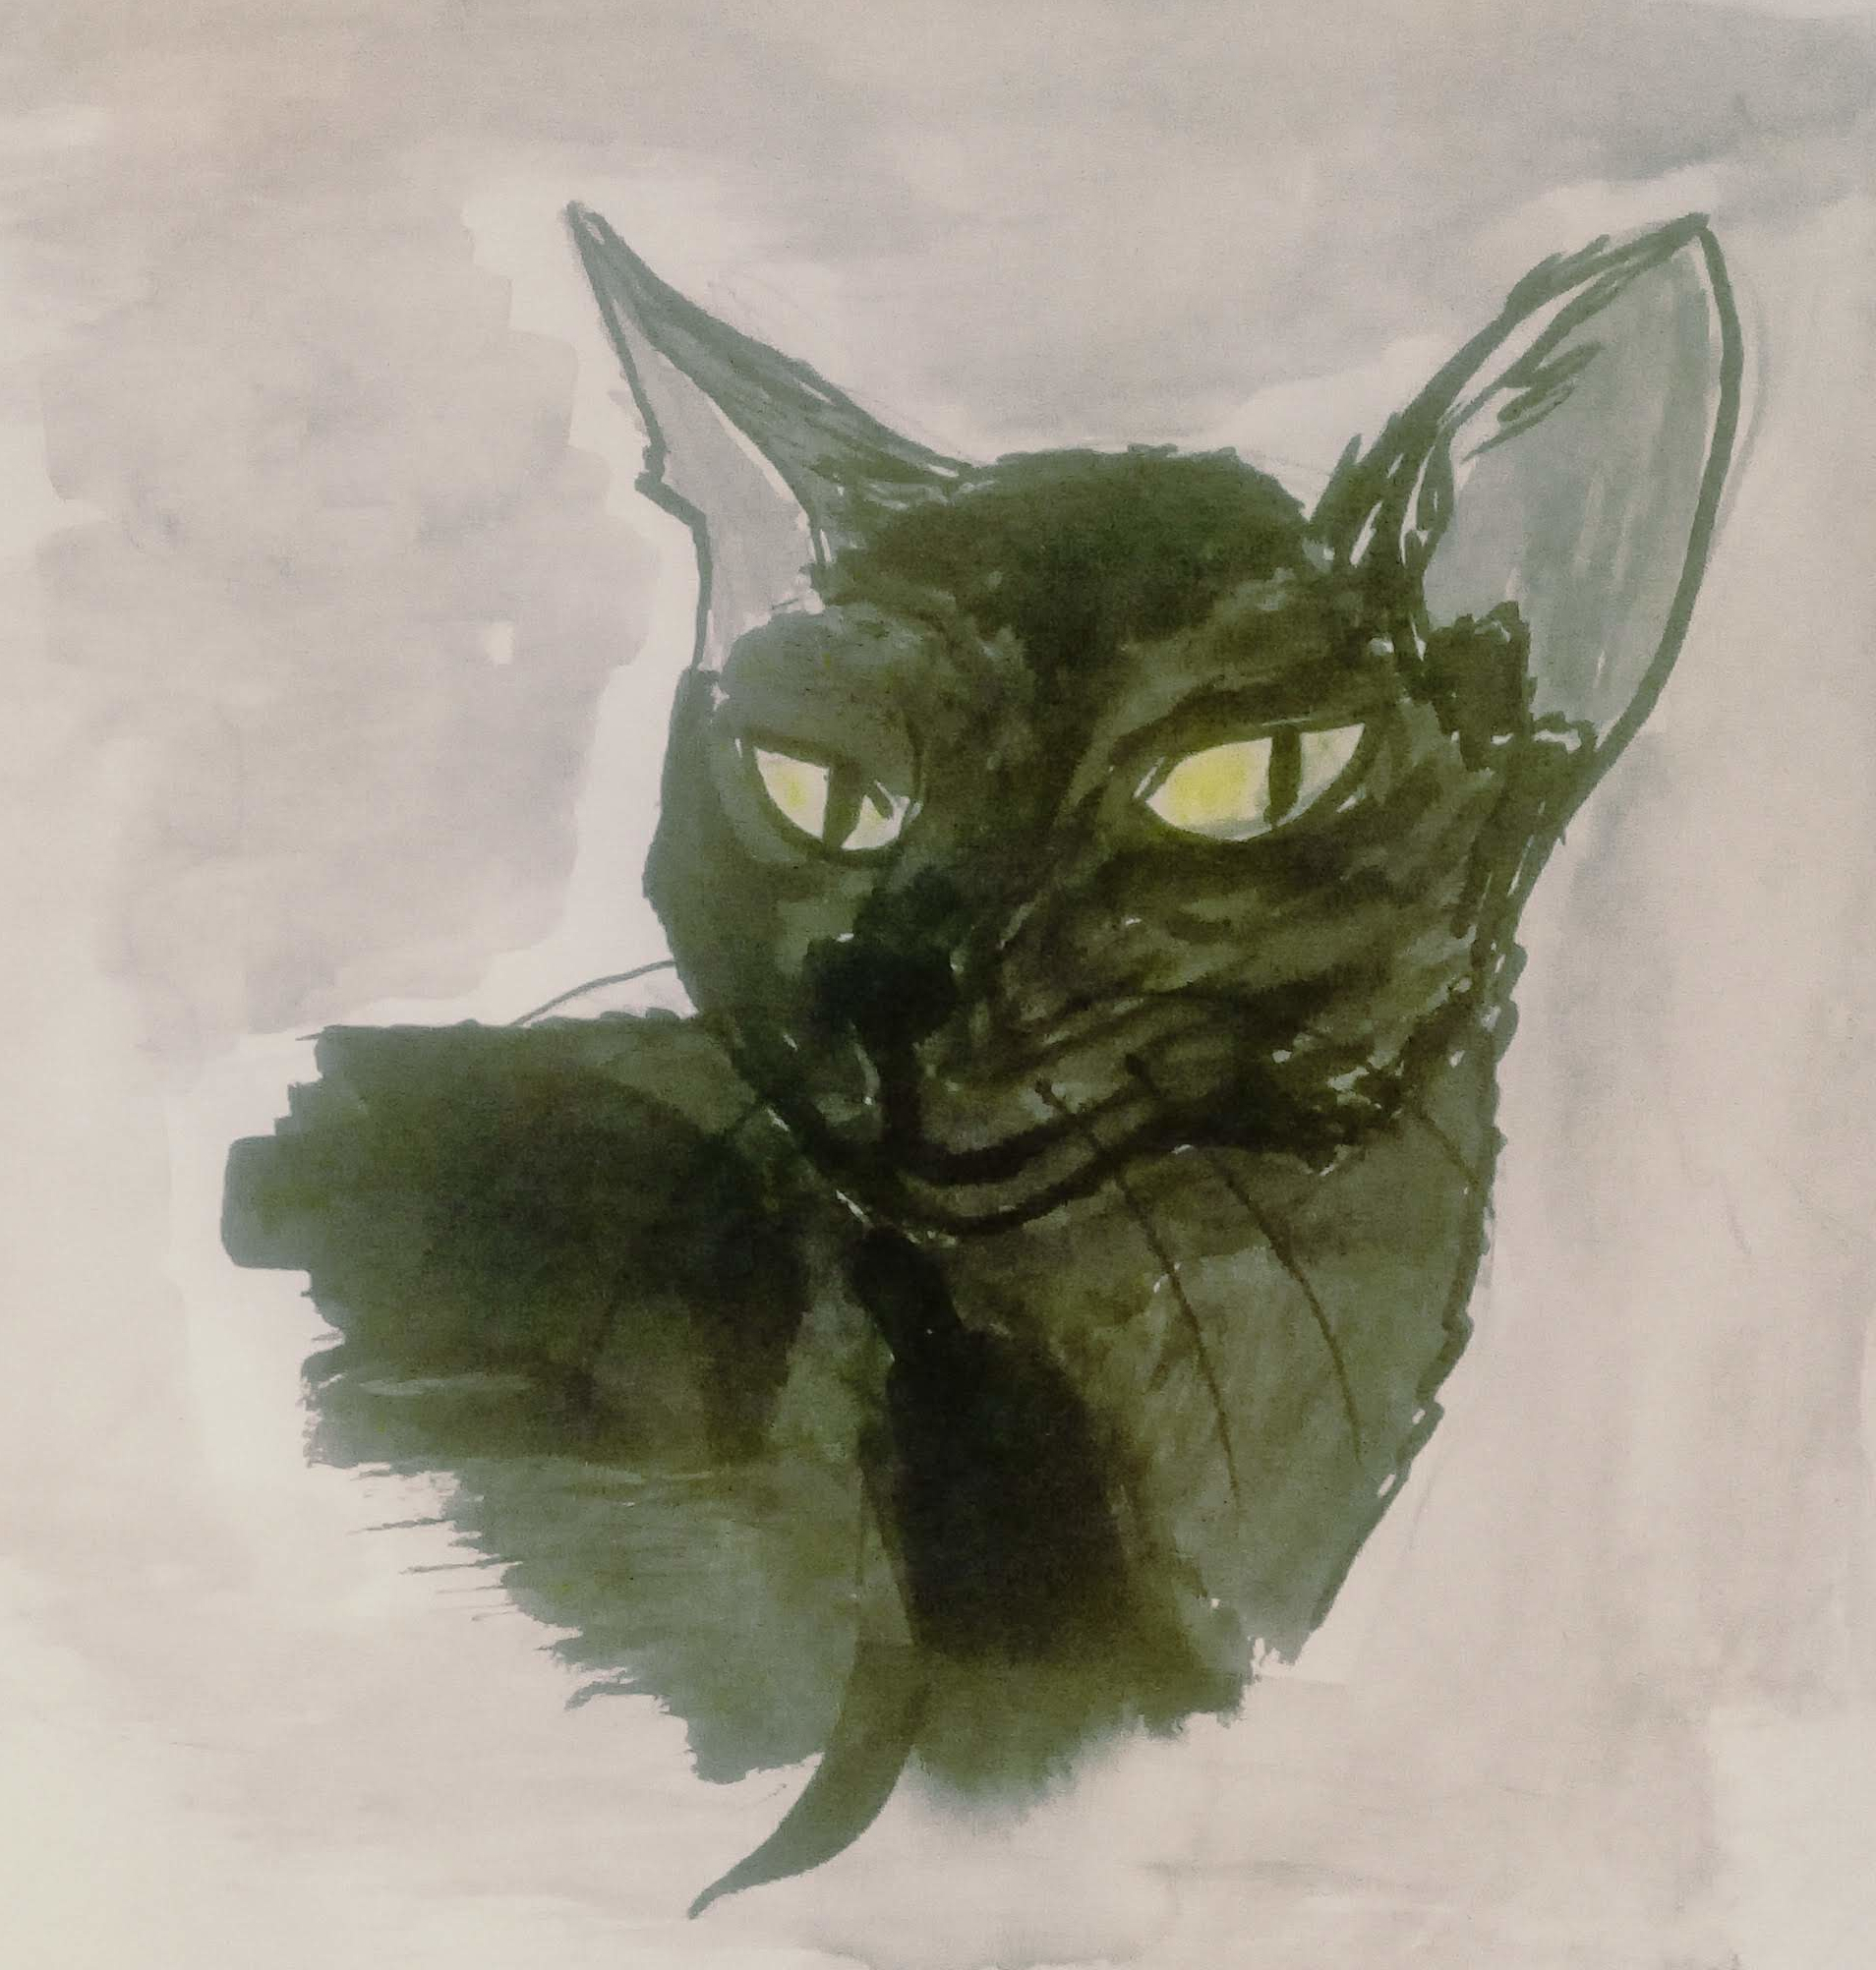
\includegraphics[width=.45\textwidth,trim=0cm 0cm 0.cm 0cm,clip]{frente_al_chino}
\end{wrapfigure}     
BANQUETE FENOMENAL DE COMIDA CHINA. POR UN INSTANTE, MEDÍ LAS POSIBILIDADES DE ROBAR GRACIAS A MIS PODEROSOS RECURSOS FELINOS. MÁS DE UNA VEZ HABÍA CONSEGUIDO EN CASA PEDACITOS DE JAMÓN, DE QUESO, DE PIZZA, DE POLLO, BUENO, ¡Y ALGUNA COSA MÁS DE LA QUE AÚN NO SE DIERON CUENTA! 








\newpage

\begin{tikzpicture}[remember picture, overlay]
	
	\node [inner sep=0pt, minimum width=\paperwidth, minimum height=\paperheight] at (current page.center) {
\includegraphics[width=\paperwidth,height=\paperheight,angle=0]{paper7}};
\end{tikzpicture}
\begin{wrapfigure}{r}{.35\textwidth}
	\includegraphics[width=.27\textwidth,trim=0cm 0cm 0cm 0cm,clip]{uñas}
\end{wrapfigure}
SEGUÍA LOS MOVIMIENTOS EN TORNO A LA COMIDA CUANDO MIS SENTIDOS

GATUNOS ME INDICARON QUE OTRO HUMANO SE ACERCABA.

MIRÉ CON EL COSTADO DE MIS OJOS Y ALCANCÉ A DETECTAR UNA SEÑORA DE VOZ 
ALGO ESTRIDENTE ¡QUE PARECÍA QUE ME HABLABA A MÍ!

%		\node[text width=15cm,xshift=-4cm] at (current page.center){
	-AY, ¡PERO MIRÁ ESTE NEGRITO 
	
	TODO BONITO!
	
	VI ACERCARSE UNA GARRA HUMANA. 
	
	¡NUNCA HABÍA VISTO NADA SEMEJANTE!
	
	
	%};


\newpage
\begin{tikzpicture}[remember picture, overlay]
	\node [inner sep=0pt, minimum width=\paperwidth, minimum height=\paperheight] at (current page.center) {\includegraphics[width=\paperwidth,height=\paperheight,angle=0]{uñas2}};
\end{tikzpicture}			
ME ARQUEÉ TODO DEL SUSTO, CON LOS PELOS ERIZADOS, PARA AVISAR QUE YO IBA A USAR LAS MÍAS.		
PERO LA SEÑORA QUE TENÍA LAS GARRAS, SONREÍA Y NO PARECÍA QUERER ATACARME.

-ESTÁ SOLITO, ¡MIRALO! ¿SE HABRÁ PERDIDO?
\newline
\vspace{.35\textheight}
- ¡MAMÁ, DEJALO, ¿NO VES QUE ES MEDIO SALVAJE?

UNA NIÑA ACOMPAÑABA A LA DAMA DE GARRAS AZULES.		
PARECÍA ENTENDER MEJOR A LOS FELINOS.

- ¡AY, BUENO! ¡QUÉ CARÁCTER! 

POR LAS DUDAS, ME FUI PRUDENTE PARA NO TENER PROBLEMAS.
\newpage
\begin{tikzpicture}[remember picture, overlay]
	\node [inner sep=0pt, minimum width=\paperwidth, minimum height=\paperheight] at (current page.center) {
\includegraphics[width=\paperwidth,height=\paperheight,angle=0]{paper8}};
	\node [inner sep=0pt, minimum width=\paperwidth] at (current page.center) {\includegraphics[width=\paperwidth,angle=0]{uñas3}};
	
\end{tikzpicture}	
SEGUÍ MI CAMINO HASTA LLEGAR A UN MUY CURIOSO LOCAL. 

\begin{flushright}
	\begin{minipage}{.5\textwidth}
		ASÍ PUDE DESCUBRIR DONDE LAS PERSONAS PODÍAN TALLARSE
		ESAS GARRAS TAN RARAS Y DE COLORES. 			
		A MI ME GUSTAN MIS GARRITAS NEGRAS.	
	\end{minipage}
\end{flushright}





\newpage
\begin{tikzpicture}[remember picture, overlay]
	\node [inner sep=0pt, minimum width=\paperwidth, minimum height=\paperheight] at (current page.center) {
\includegraphics[width=\paperwidth,height=\paperheight,angle=0]{paper9}};
	\node [inner sep=0pt,  minimum height=\paperheight,xshift=4cm] at (current page.center) {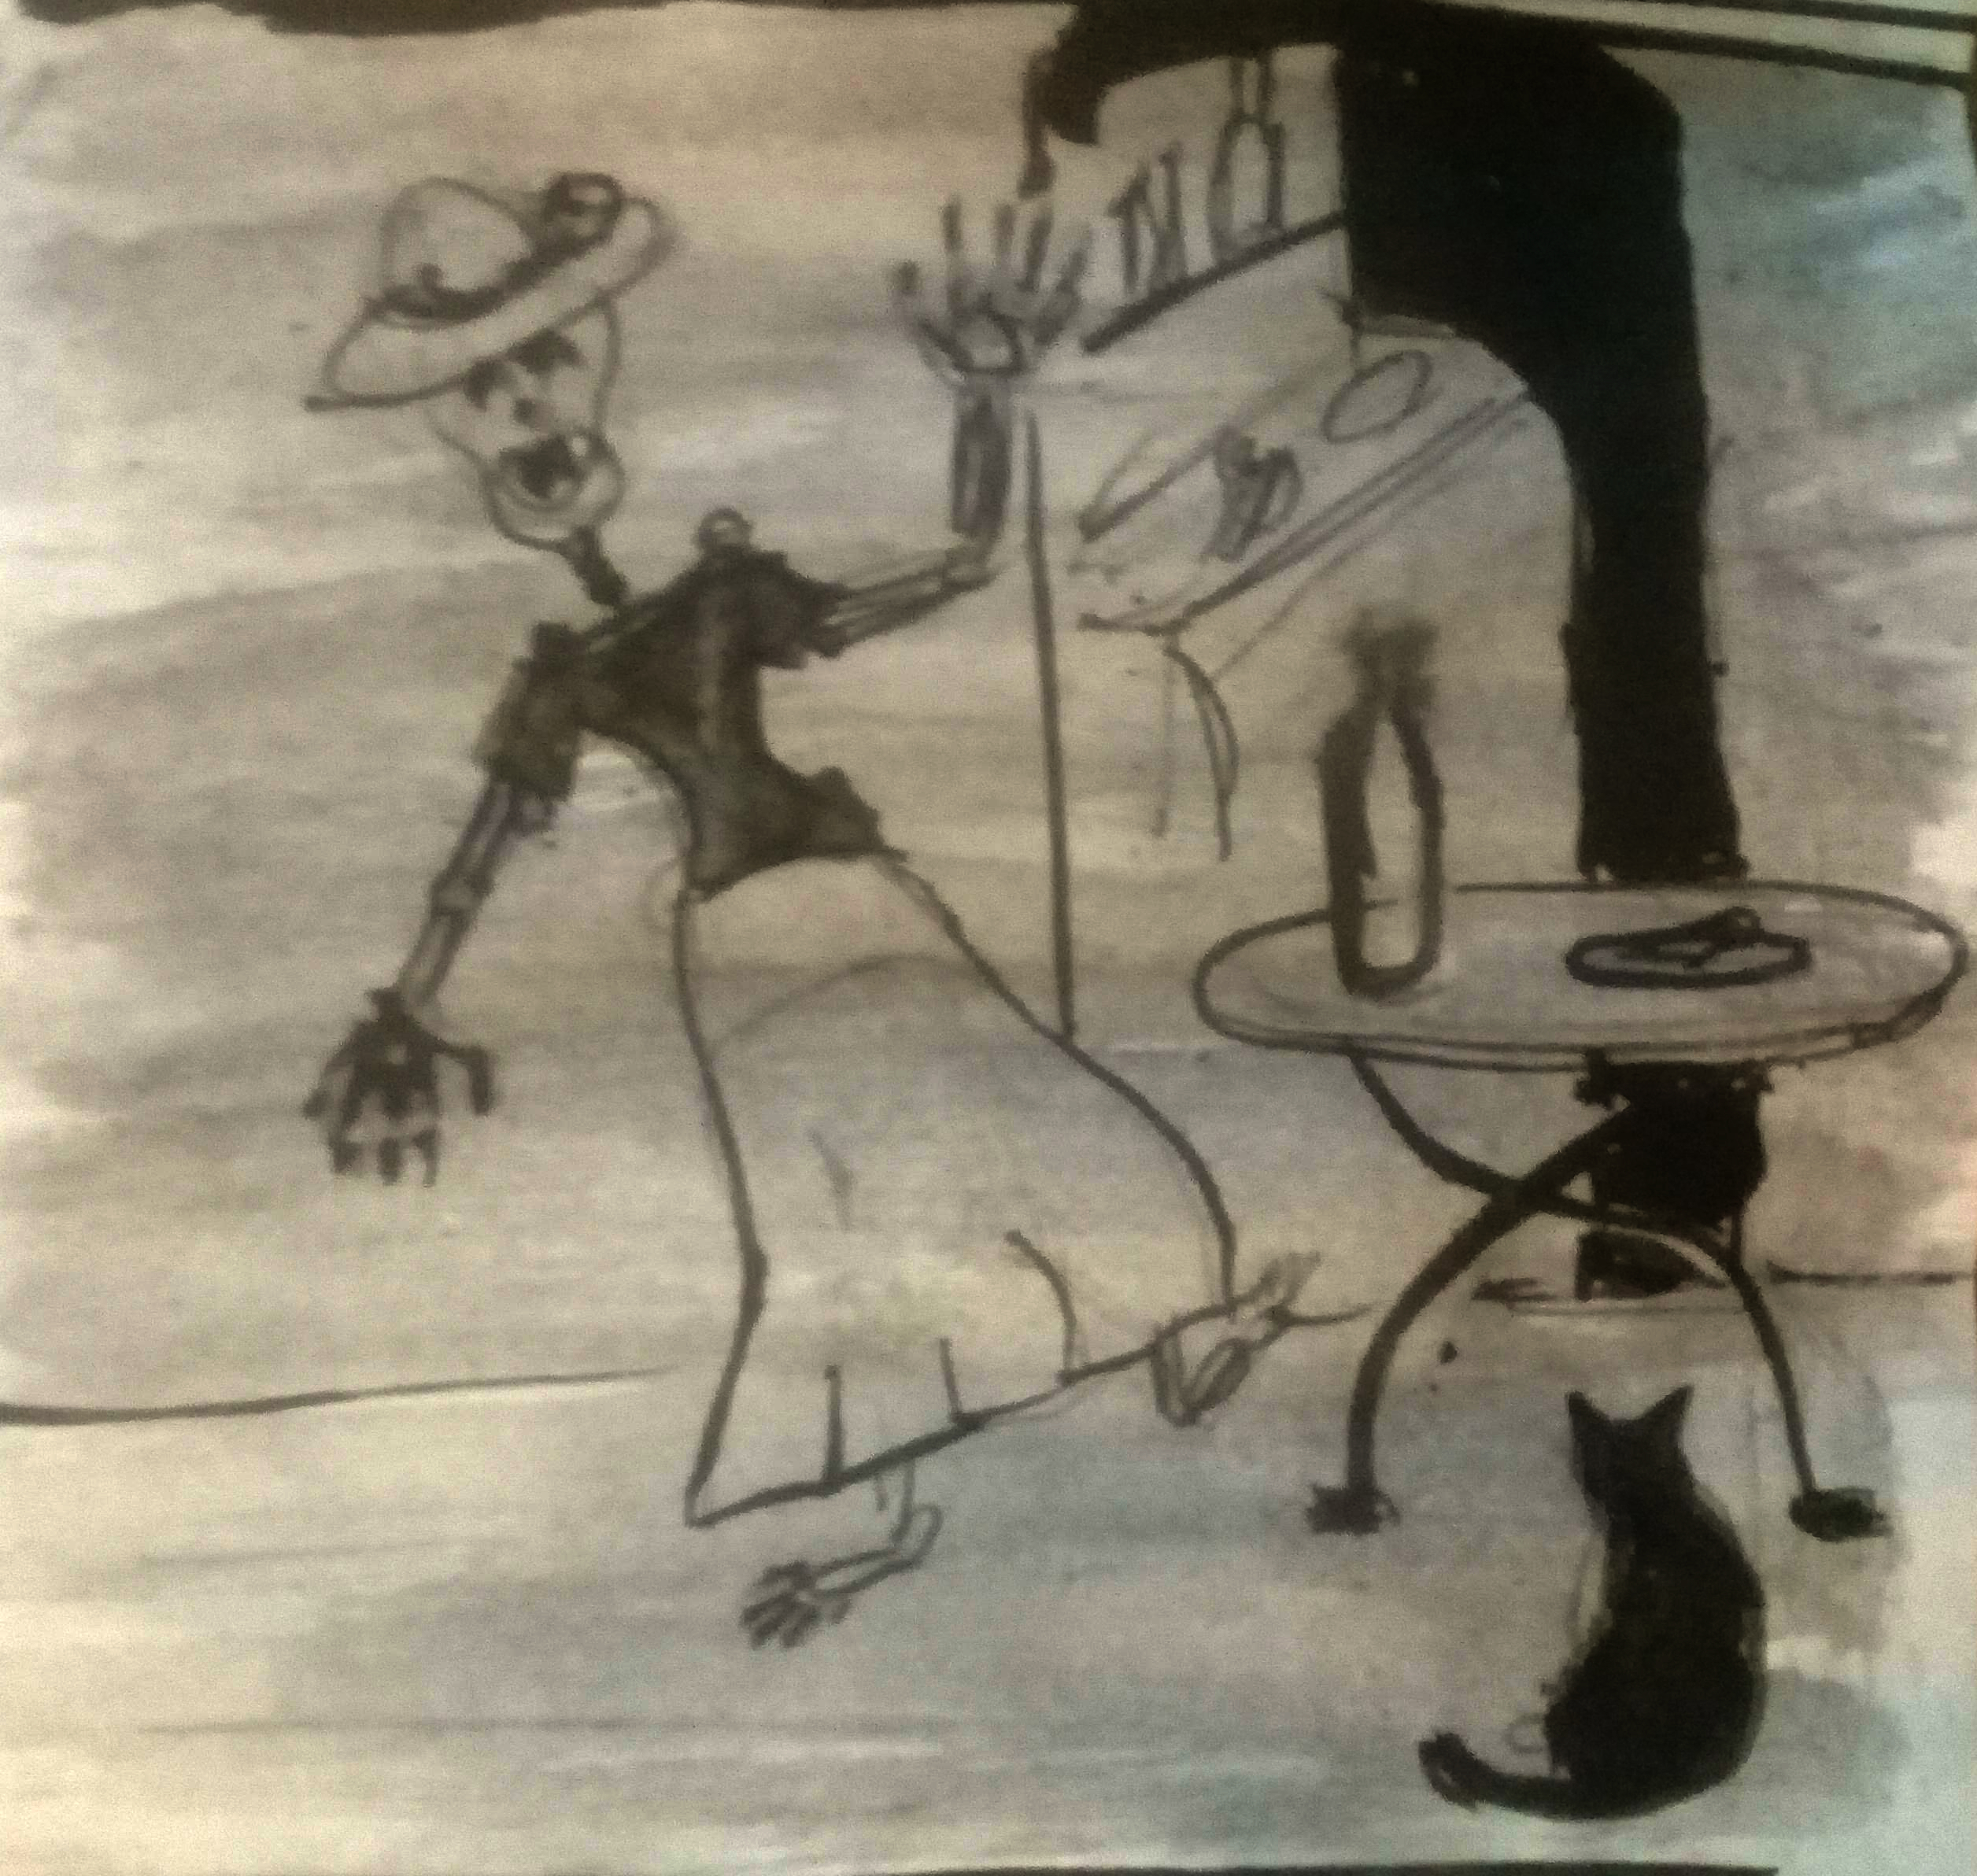
\includegraphics[height=\paperheight,angle=0]{mexicano1}};
	
\end{tikzpicture}	
\begin{minipage}{.5\textwidth}
	ALGO MUCHO MÁS INTERESANTE SE HALLABA JUSTO
	UNOS
	
	METROS
	MÁS ADELANTE. 
	
	ESQUELETOS HUMANOS 
	
	VESTIDOS SIMPÁTICAMENTE 
	
	DECORABAN LA ENTRADA A 
	
	UN RESTAURANTE.
	
	LLEGABA UN MUY 
	AGRADABLE 
	
	AROMA A COMIDA, 
	
	NADA QUE PUDIERA DAÑAR A UNA BUENA DIETA FELINA.
	
	
	
	¡ES HERMOSO! ME PROMETÍ VENIR A CENAR ALGÚN DÍA QUE PUDIERA FESTEJAR ALGO. ¡ÓRALE JUANITO!
\end{minipage}






\newpage
\begin{tikzpicture}[remember picture, overlay]
	\node [inner sep=0pt, minimum width=\paperwidth, minimum height=\paperheight] at (current page.center) {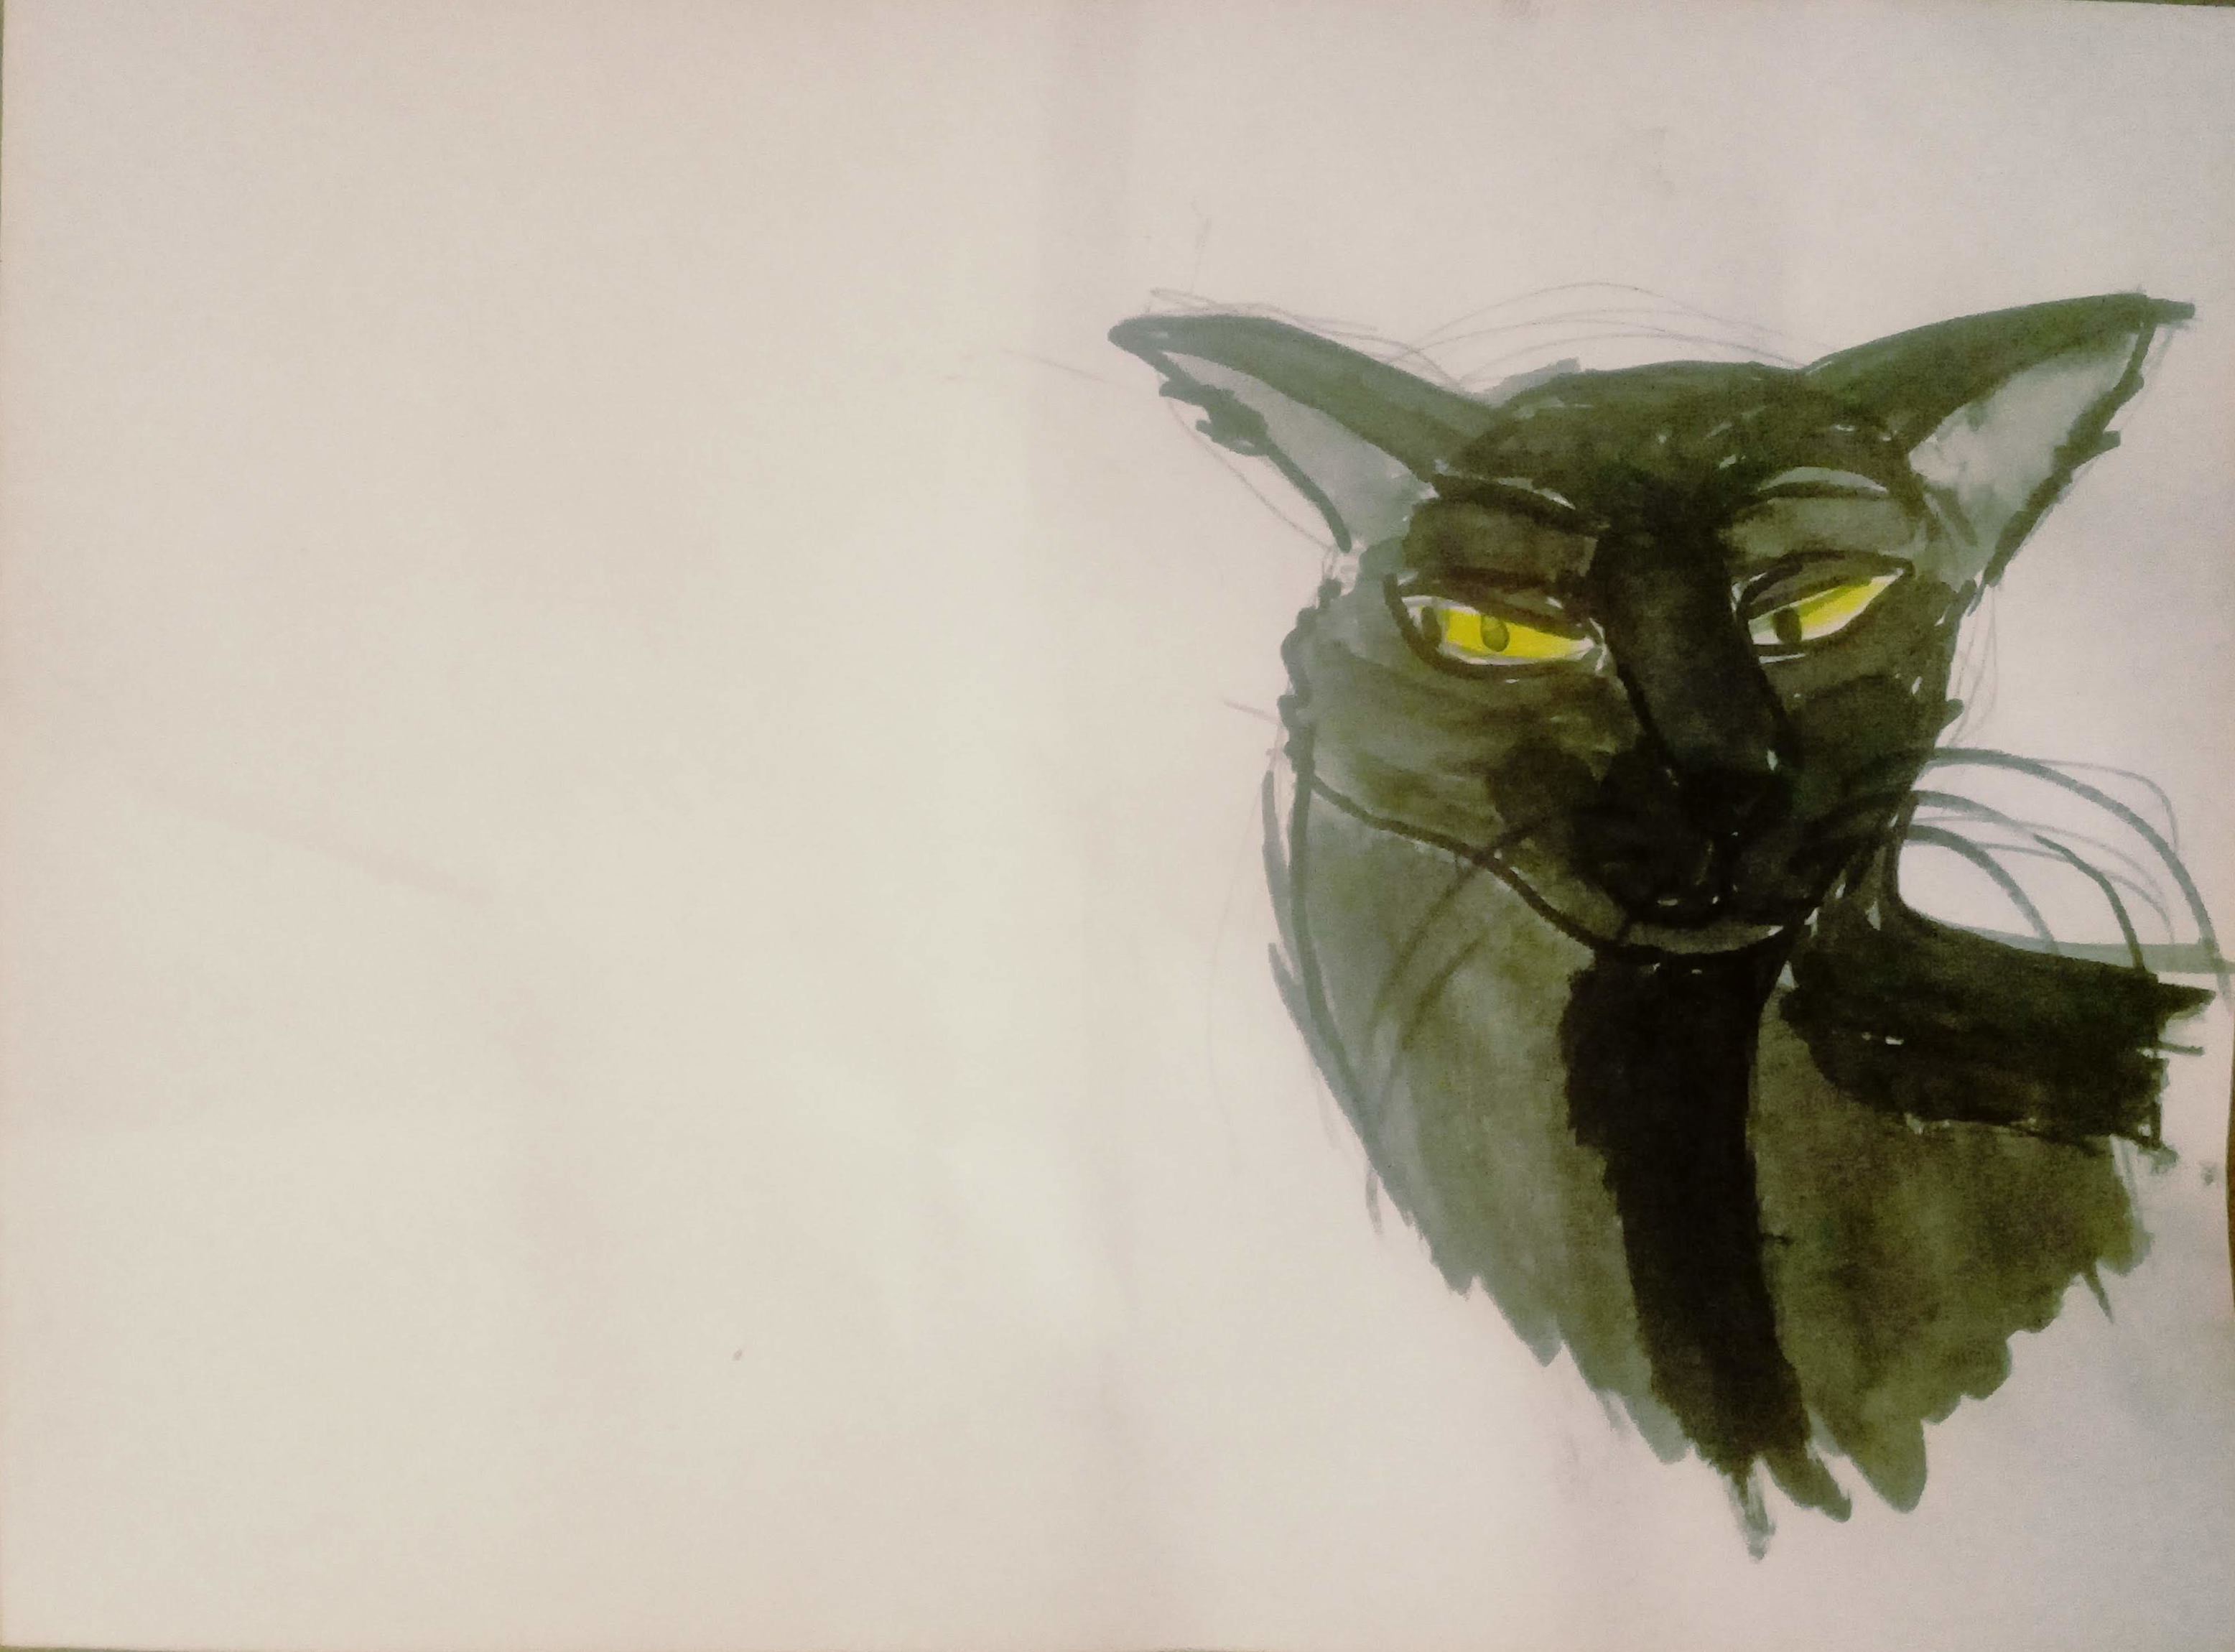
\includegraphics[width=\paperwidth,height=\paperheight,angle=0]{reflexion2}};
\end{tikzpicture}	
\begin{minipage}{.6\textwidth}	
	USTEDES SE PREGUNTARÁN COMO 
	
	CONOZCO TANTO DE GASTRONOMÍA,
	
	PUES YA 		
	COMENTÉ QUE EL CHAW 
	
	FAN 
	Y LOS 		
	BUÑUELOS DE POLLO
	SON 
	
	MUY 		
	BUENOS,				
	Y AHORA PENSANDO 
	
	EN COMER 
	ALGÚN 		
	BURRITO 		
	MEXICANO$\ldots$ 
	
	PUES DEBO 
	CONFESAR 	
	QUE MÁS DE
	
	UNA VEZ, 
	A ESCONDIDAS,	 
	HE PROBADO 
	
	DIFERENTES 
	PLATOS EN 		  
	CASA. 		  
	HACE 
	
	NO MUCHO TIEMPO ATRÁS, 
	ROBÉ UN 
	
	BUEN PEDAZO
	DE PIZZA CON JAMÓN. 
	
	¡RECIÉN SE DIERON CUENTA AL		   
	DÍA SIGUIENTE! 
	
	JEJEJE.
\end{minipage}



\newpage
\begin{tikzpicture}[remember picture, overlay]
	\node [inner sep=0pt, minimum width=\paperwidth, minimum height=\paperheight,xshift=5cm] at (current page.center) {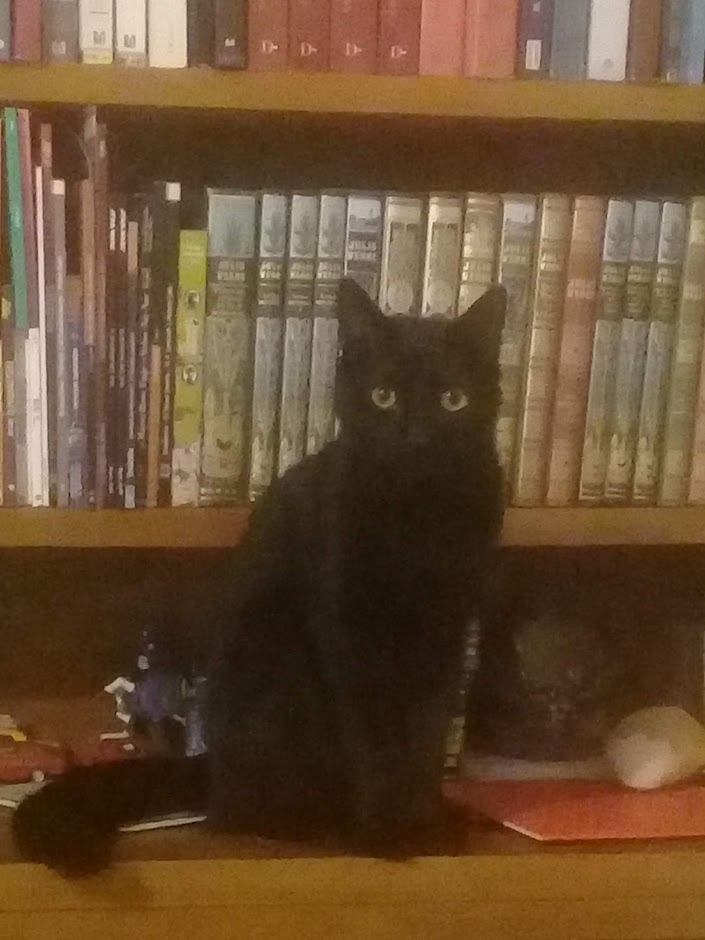
\includegraphics[ height=\paperheight,angle=0]{biblio}};
\end{tikzpicture}

\begin{minipage}{.4\textwidth}	\vspace{.3\textheight}
	OTTOKO LES RECUERDA QUE PARA ESCRIBIR HISTORIAS, HACE BIEN LEER BUENAS HISTORIAS. POR ESO SIEMPRE PASEA POR LA BIBLIOTECA!! 
\end{minipage}

\newpage
\begin{tikzpicture}[remember picture, overlay]
	\node [inner sep=0pt, minimum width=\paperwidth, minimum height=\paperheight] at (current page.center) {
\includegraphics[width=\paperwidth,height=\paperheight,angle=0]{paper10}};
	\node [inner sep=0pt,  minimum height=\paperheight,xshift=7cm] at (current page.center) {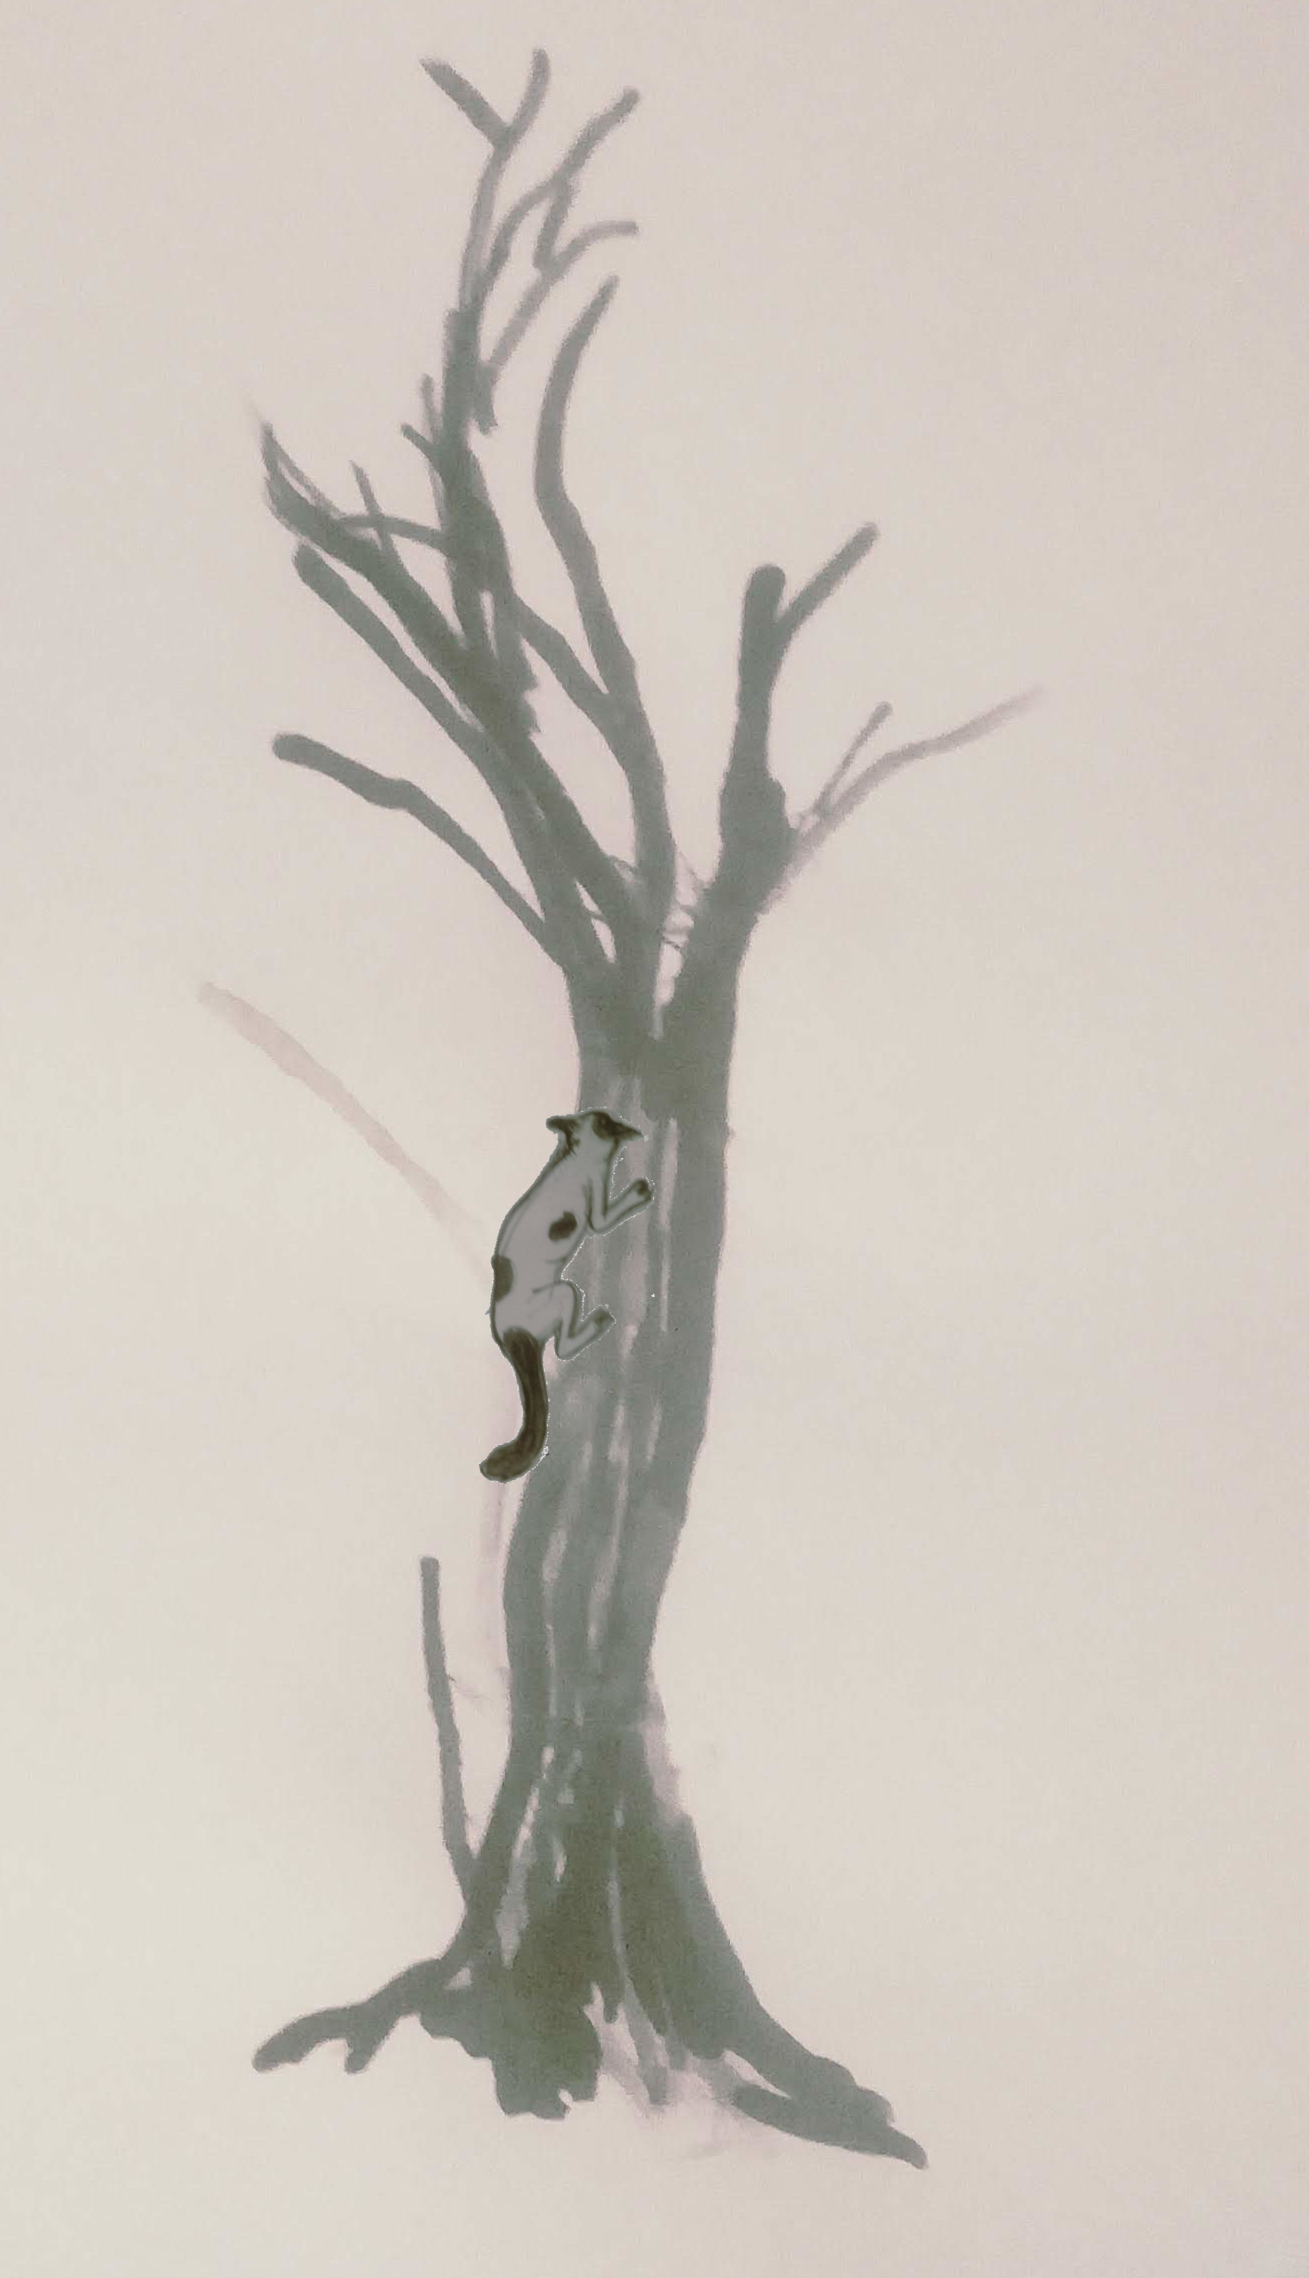
\includegraphics[height=\paperheight,angle=0]{akis_trepa}};
\end{tikzpicture}
\begin{minipage}{.5\textwidth}
	FRENTE AL RESTAURANTE MEXICANO, HABÍA UN ÁRBOL NO MUY VISTOSO. DE REPENTE, ESCUCHÉ BAJAR A UN GATO. Y ENSEGUIDA VOLVIÓ A SUBIR AL ÁRBOL. REPITIÓ ESTE SUBE Y BAJA MÁS DE TRES VECES. PARECÍA NO IMPORTARLE MI PRESENCIA NI LA DE NADIE. TENÍA MUCHA SEGURIDAD PARA DESPLAZARSE. PARECÍA UN GATO DE EXPERIENCIA, DIGAMOS UNOS 5 O 6 AÑOS DE EDAD, ¡HAGAN LA CUENTA PARA SABER SU EDAD GATUNA! 
\end{minipage}
\newpage
\begin{tikzpicture}[remember picture, overlay]
	\node [inner sep=0pt, minimum width=\paperwidth, minimum height=\paperheight] at (current page.center) {
\includegraphics[width=\paperwidth,height=\paperheight,angle=0]{paper9}};
	
\end{tikzpicture}	
ME HABÍA QUEDADO OBSERVANDO AL CURIOSO FELINO. TENÍA COLOR BLANCO Y MARRÓN CLARO, EN ESPECIAL, LAS OREJAS, LA COLA Y UN OJO. COMO YO LO MIRABA CON FIJEZA, SE DETUVO POR UN INSTANTE Y CLAVÓ SUS OJOS VERDES EN MÍ.

- EH! JOVENCITO, ¡YO NO DOY LECCIONES DE ESCALADA GRATIS! 

- LA VERDAD ES QUE NO ENTIENDO LO QUE HACÉS, ¿PARA QUÉ BAJAR Y SUBIR TANTO?

- AFILO MIS GARRAS A LA VEZ QUE ME EJERCITO, NO TE VENDRÍA MAL PRACTICAR UN POCO.

- PUES YO HAGO MI AFILADA DE GARRAS ASÍ, DIJE MOSTRANDO UN RASQUETEO ENÉRGICO SOBRE LA BASE DEL TRONCO DEL ÁRBOL.

- ESO ESTÁ BIEN, PERO SÍ TE DOY UN CONSEJO GRATIS, TREPANDO CON FUERZA ADEMÁS GANÁS FUERZA.

- ¡PUES, GRACIAS!, DIJE, ¿CÓMO TE LLAMÁS?

\newpage
\begin{tikzpicture}[remember picture, overlay]
	\node [inner sep=0pt, minimum width=\paperwidth, minimum height=\paperheight] at (current page.center) {
\includegraphics[width=\paperwidth,height=\paperheight,angle=0]{paper11}};
	\node [inner sep=0pt,  minimum height=\paperheight,xshift=.25\textwidth,yshift=.1\textheight] at (current page.center){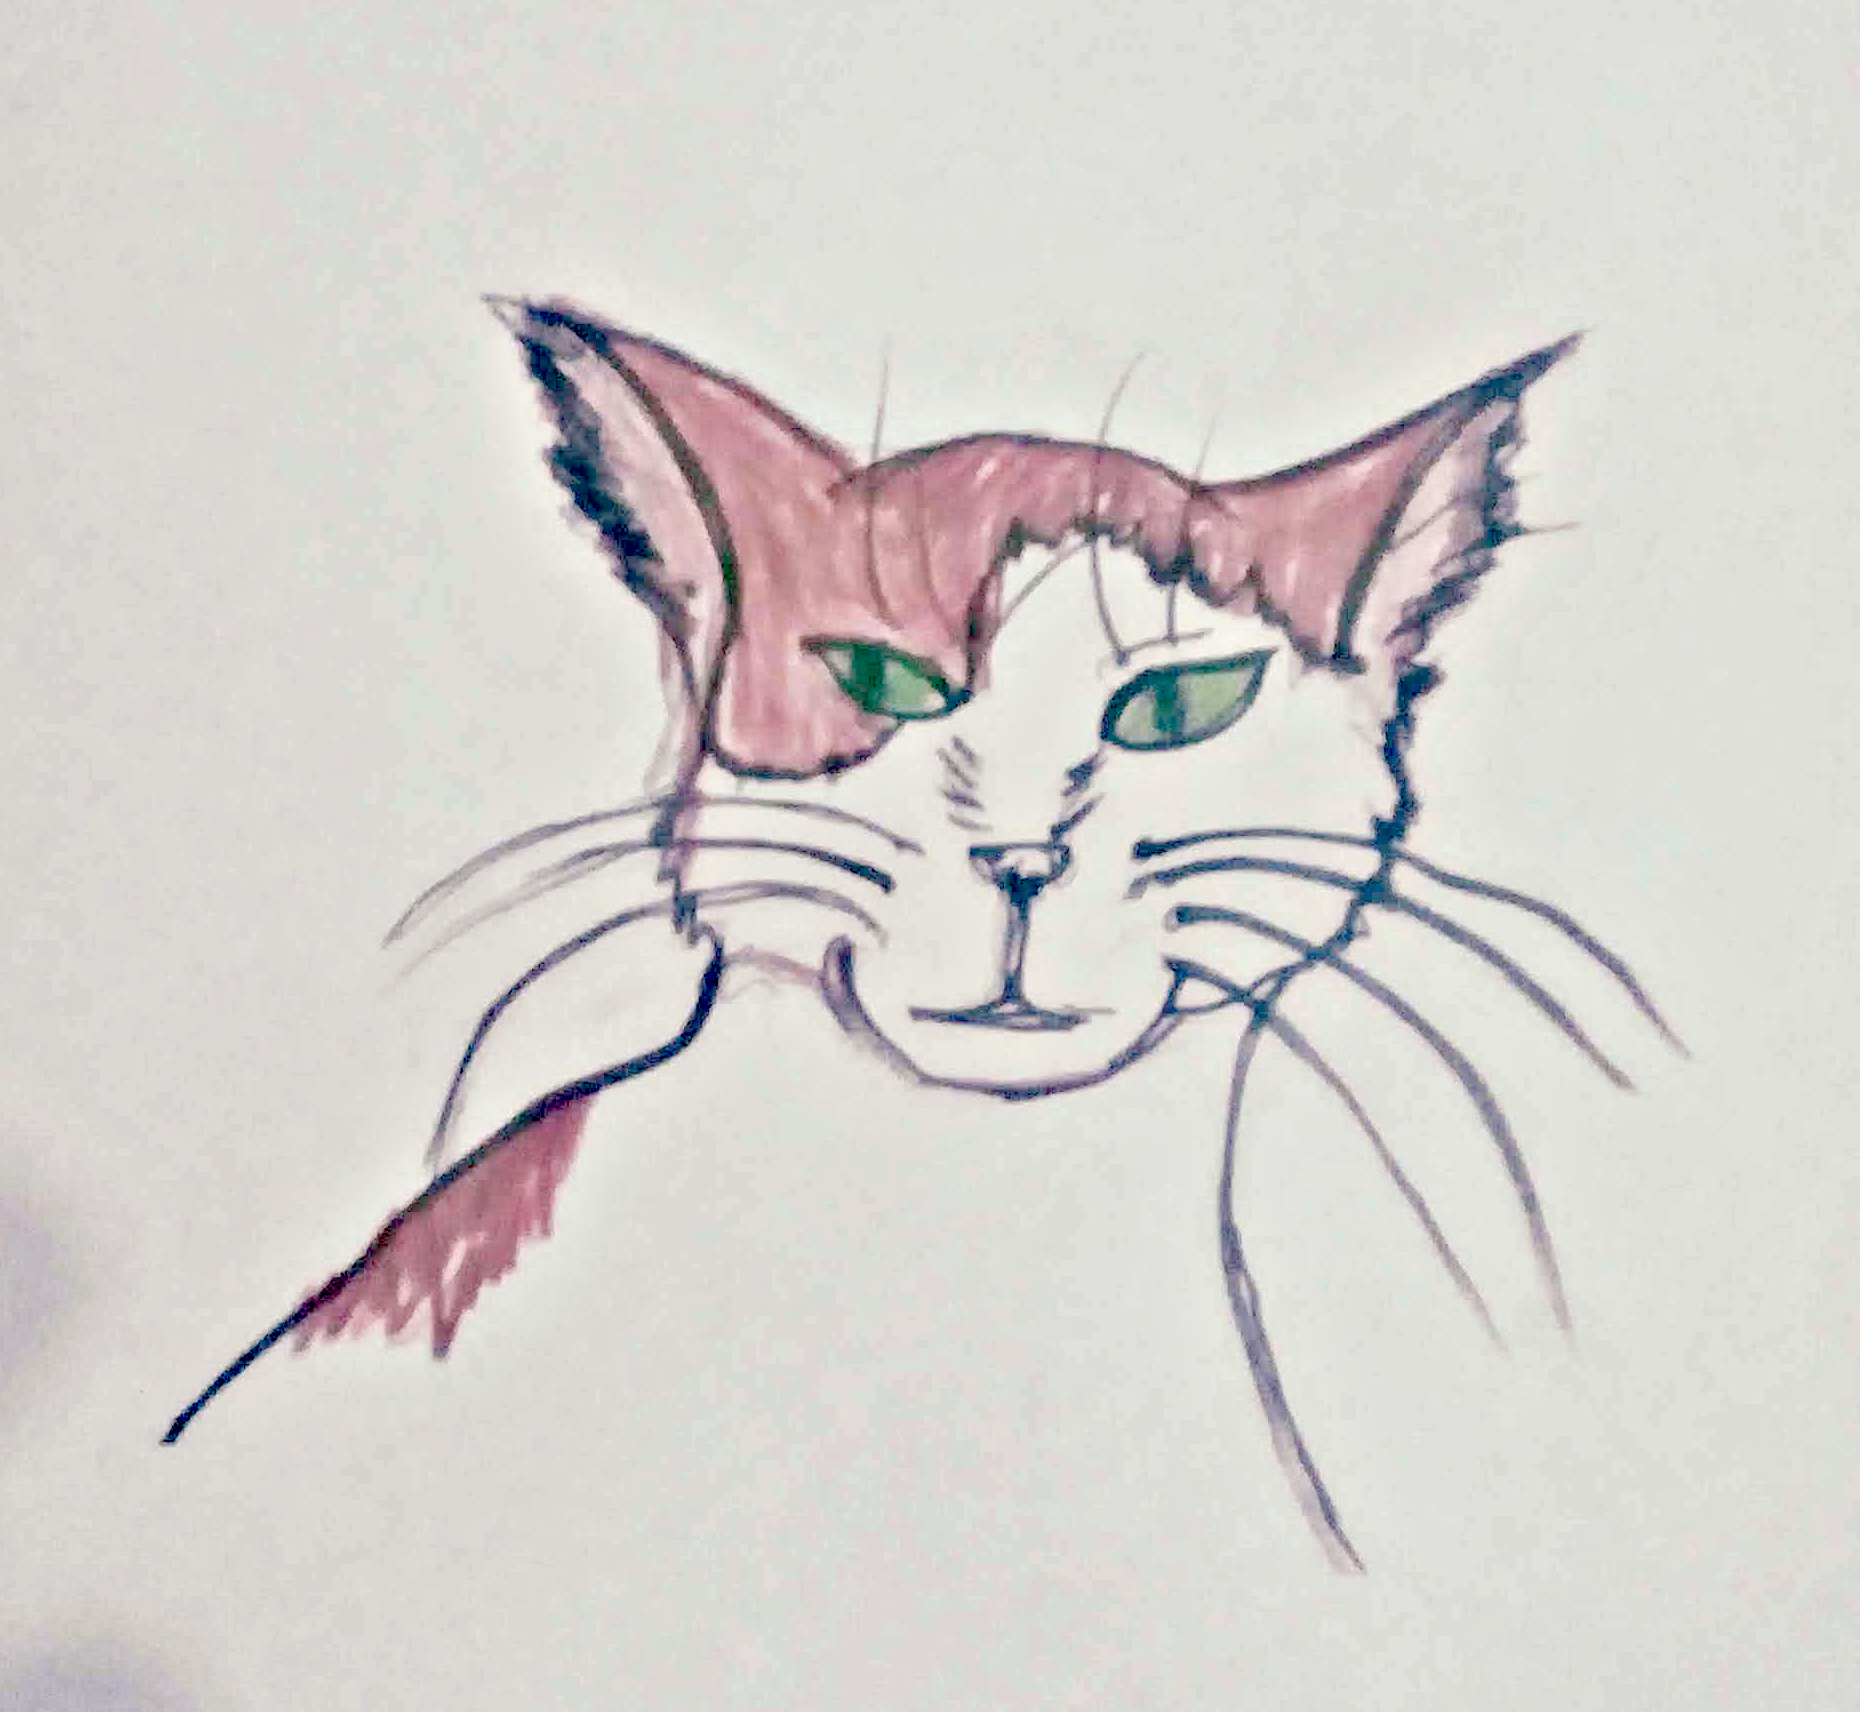
\includegraphics[height=.8\paperheight,angle=0]{akis_rostro}};
\end{tikzpicture}
\begin{minipage}{.5\textwidth}
	- MI NOMBRE ES AKIS, ¿CUAL ES EL TUYO? ¿ESTÁS ALGO PERDIDO?
	
	- ME LLAMO OTTOKO, Y NO, SÓLO ESTOY CONOCIENDO UN POCO EL BARRIO, VIVO ACÁ CERCA EN ESA CASA DE ALLÁ, ¿Y VOS?
	
	- ¡AH!, YO NO TENGO UNA SÓLA CASA, VIVO UN POCO EN CADA UNA. HAY UNAS PERSONAS QUE LES
	
	GUSTA ALIMENTAR GATOS COMO 
	
	YO. SI QUERÉS, TE PUEDO ACOMPAÑAR UN POCO, ME VENDRÍA BIEN UN PASEO.
	
	¡NO SABÍA QUE HACER! ¿SERÍA UN GATO DE CONFIAR? 
\end{minipage}	

\newpage
\begin{tikzpicture}[remember picture, overlay]
	\node [inner sep=0pt, minimum width=\paperwidth, minimum height=\paperheight] at (current page.center) {
\includegraphics[width=\paperwidth,height=\paperheight,angle=0]{paper11}};
\end{tikzpicture}
- EHH... PUES NO SÉ...

- ENTIENDO QUE COMO GATO JOVEN AÚN TENGAS TUS PRECAUCIONES. VEO QUE NO TRAÉS NI COLLAR NI CHAPITA DE IDENTIFICACIÓN, HUM!

- ¡AH! ¡ES VERDAD! ME DIJERON QUE NO SABÍAN CUAL COLOR ELEGIR$\ldots$ ¡PERO VOS TAMPOCO!

- ES QUE YO ME PERDÍ HACE TIEMPO, Y ELEGÍ QUEDARME POR ESTE BARRIO. ANTES VIVÍA EN UNA CASA CON JARDÍN. ¡AHORA TODOS LOS PARQUES DEL BARRIO SON MIS JARDINES! ¡Y HE COMIDO SOBRAS DE LOS MÁS ELEGANTES RESTAURANTES!

¡QUÉ PRESUMIDO!, PENSÉ. Y LUEGO AKIS AGREGÓ:

- SI QUERÉS, PODEMOS IR A PASEAR A UNA DE MIS CASAS, HAY LUGARES PARA EMBOSCAR PALOMAS, RATAS ESCONDIDAS  EN DESAGÜES Y SEGURAMENTE VARIAS CUCARACHAS. -LO DIJO CON AIRE SOBRADOR, ¡PERO REALMENTE LA PROPOSICIÓN ERA MUY TENTADORA!



\newpage
\begin{tikzpicture}[remember picture, overlay]
	\node [inner sep=0pt, minimum width=\paperwidth, minimum height=\paperheight] at (current page.center) {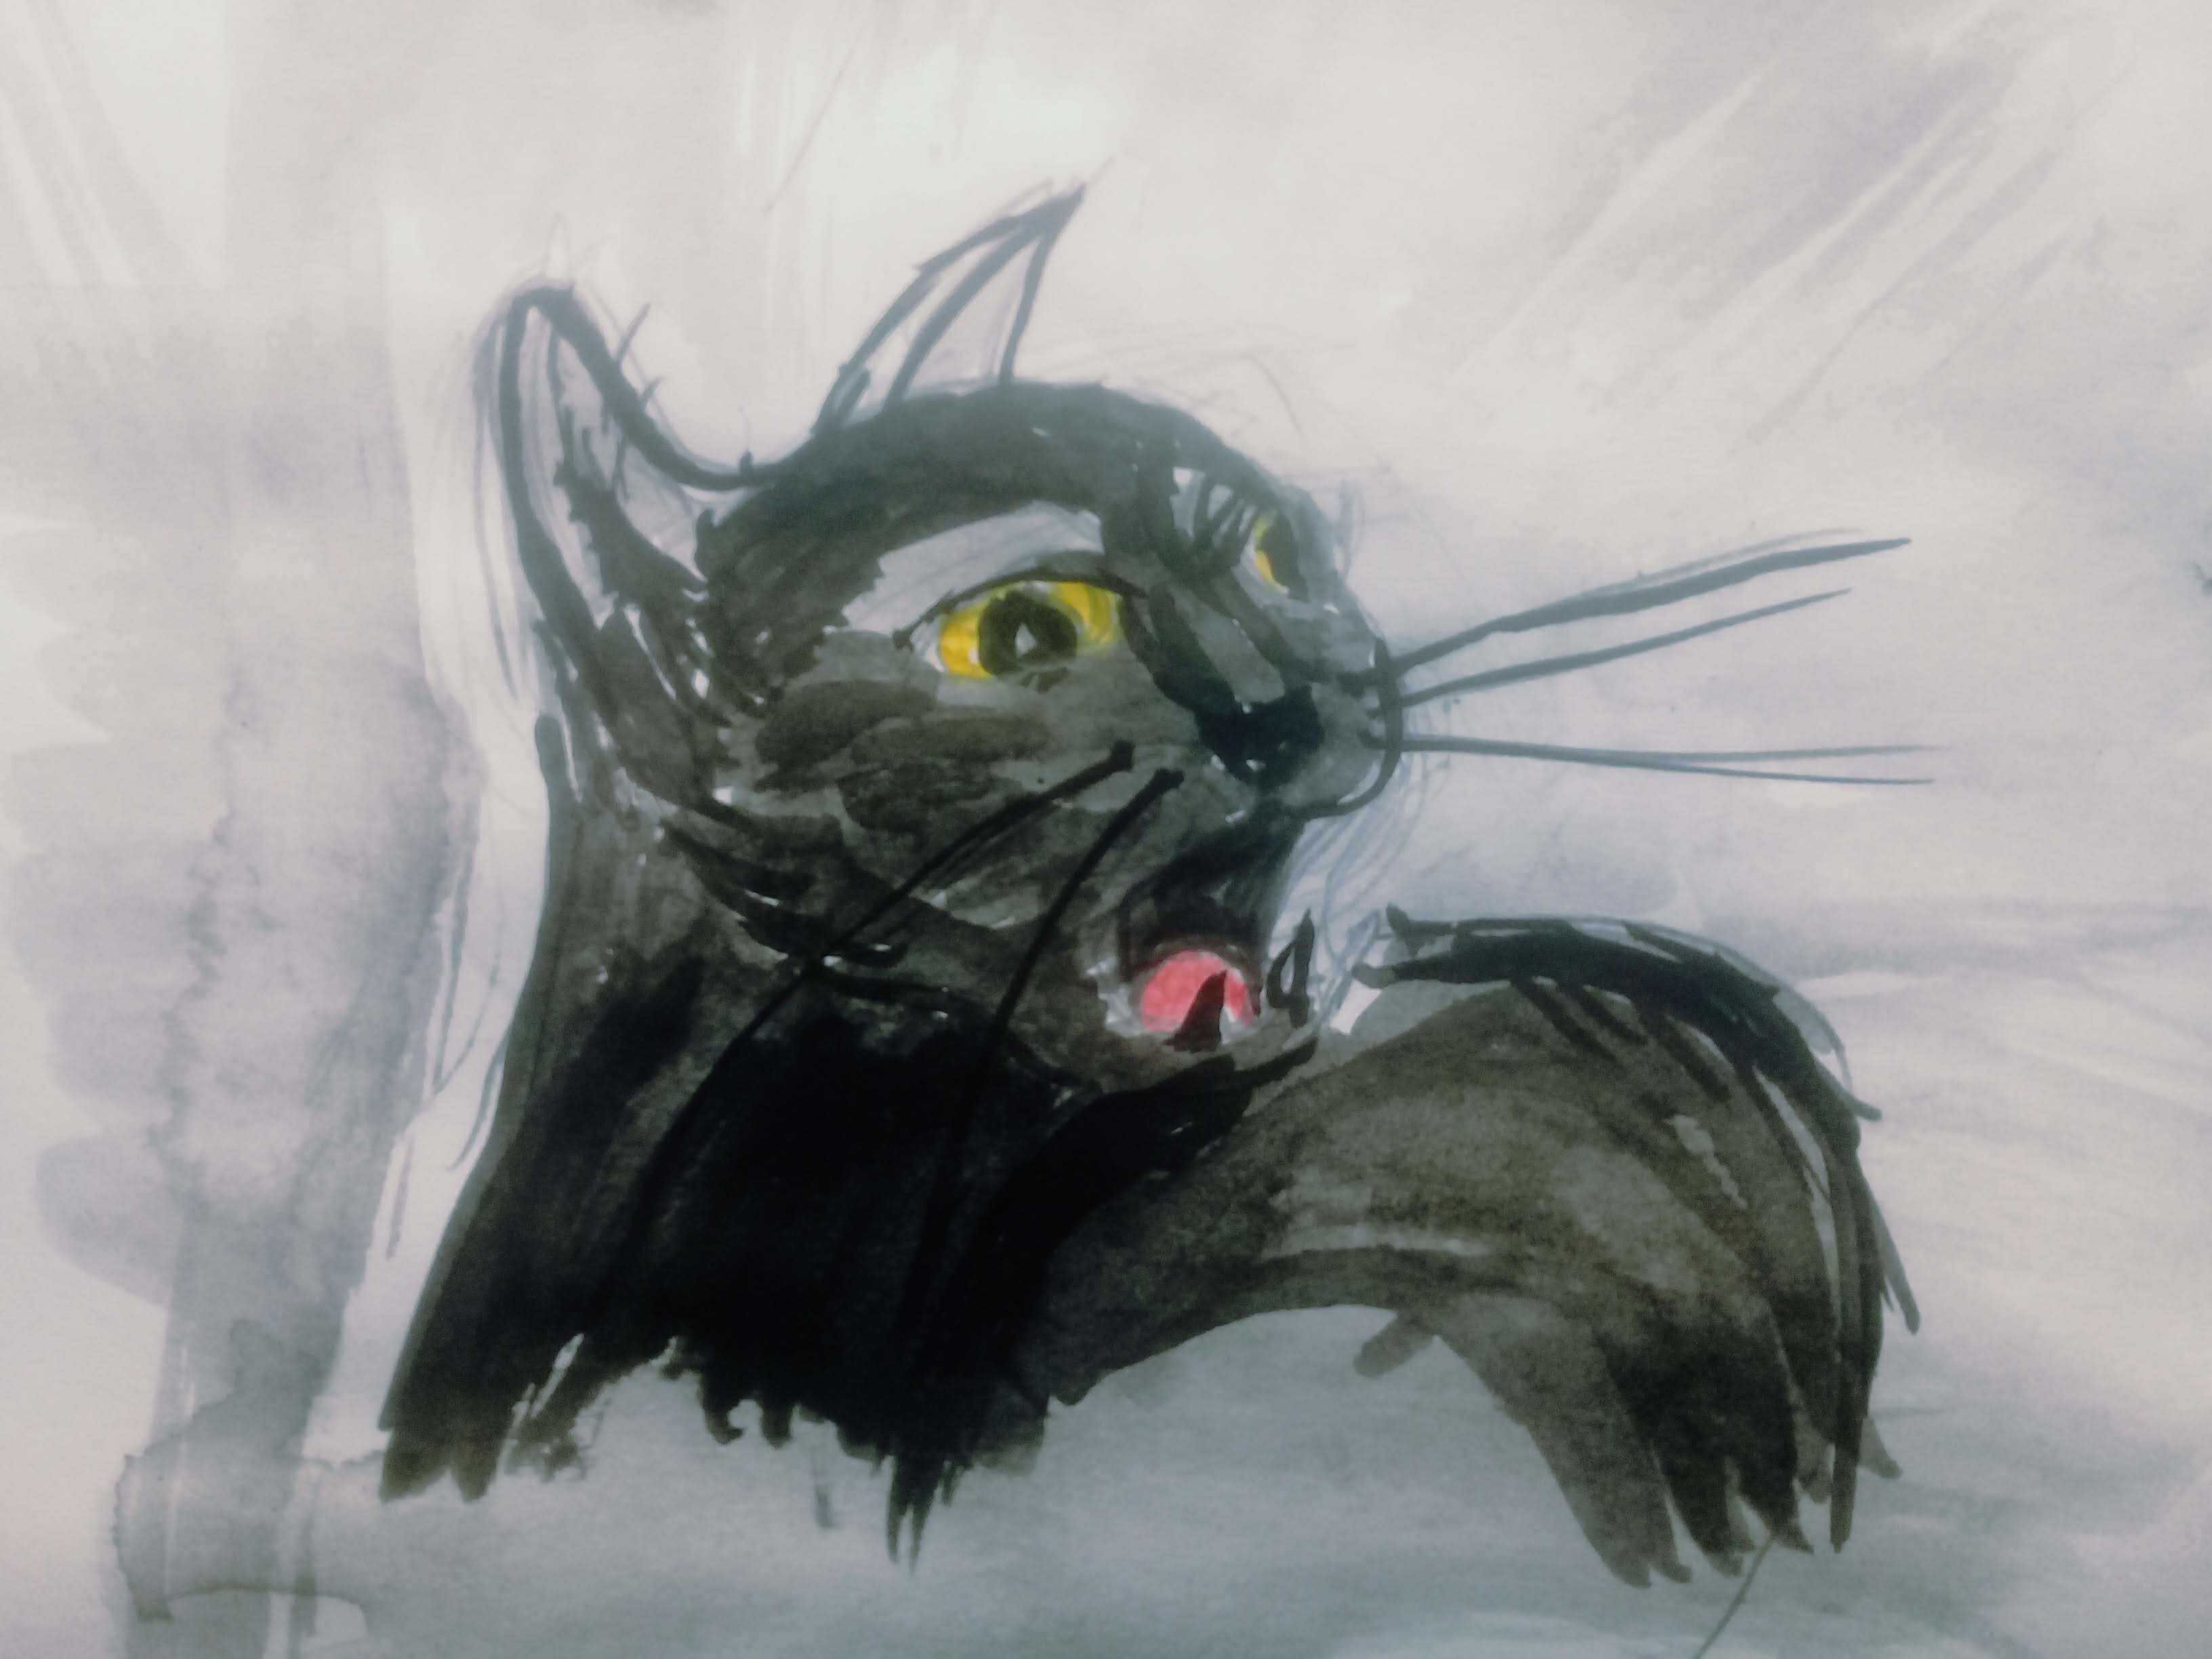
\includegraphics[width=\paperwidth,height=\paperheight,angle=0]{ottoko_sorpresa}};
\end{tikzpicture}
\newpage
\begin{tikzpicture}[remember picture, overlay]
	\node [inner sep=0pt, minimum width=\paperwidth, minimum height=\paperheight] at (current page.center) {
\includegraphics[width=\paperwidth,height=\paperheight,angle=0]{paper11}};
\end{tikzpicture}
\vspace{.3\textheight}


\begin{LARGE}
	¿PODÉS AYUDAR A OTTOKO?
\end{LARGE}

SI DECIDÍS ACOMPAÑAR A AKIS, ESCRIBE ´´1´´

SI PREFERÍS QUE OTTOKO CONTINÚE SU PASEO SOLO, ESCRIBE  ´´ 2´´ 





\newpage
\begin{tikzpicture}[remember picture, overlay]
	\node [inner sep=0pt, minimum width=\paperwidth, minimum height=\paperheight] at (current page.center) {
\includegraphics[width=\paperwidth,height=\paperheight,angle=0]{paper11}};
\end{tikzpicture}
- TAL VEZ OTRO DÍA, AKIS. POR HOY QUIERO DESCUBRIR LAS CALLES SOLO.

- A LA ORDEN, PEQUEÑO, ¡QUE TE APROVECHE EL DÍA!

Y ASÍ, EL GATO DE DOS COLORES VOLVIÓ A SUBIR Y A BAJAR SU ÁRBOL.

CONTINUÉ HASTA LLEGAR A LA ESQUINA DONDE HABÍA MUCHOS AUTOS Y MOVIMIENTO. A MI DERECHA ESTABA UNA ESTACIÓN DE SERVICIO, DONDE SE CARGA EL COMBUSTIBLE DE LOS AUTOS. OLÍA FUERTE A NAFTA, UN AROMA NO MUY AGRADABLE. TENÍA QUE MOVERME CON CUIDADO PUES LOS AUTOS CIRCULABAN POR ENCIMA DE LA VEREDA.

LLEGUÉ HASTA EL PRIMER ARBUSTO, DONDE HABÍA UN CARTEL MUY CURIOSO, COMO SI FUERA UNA PERSONA CON CABEZA DE RUEDA, Y CON UN BRAZO MÁS LARGO QUE EL OTRO, COMO INVITANDO A DETENERSE.



\newpage
\begin{tikzpicture}[remember picture, overlay]
	\node [inner sep=0pt, minimum width=\paperwidth, minimum height=\paperheight] at (current page.center) {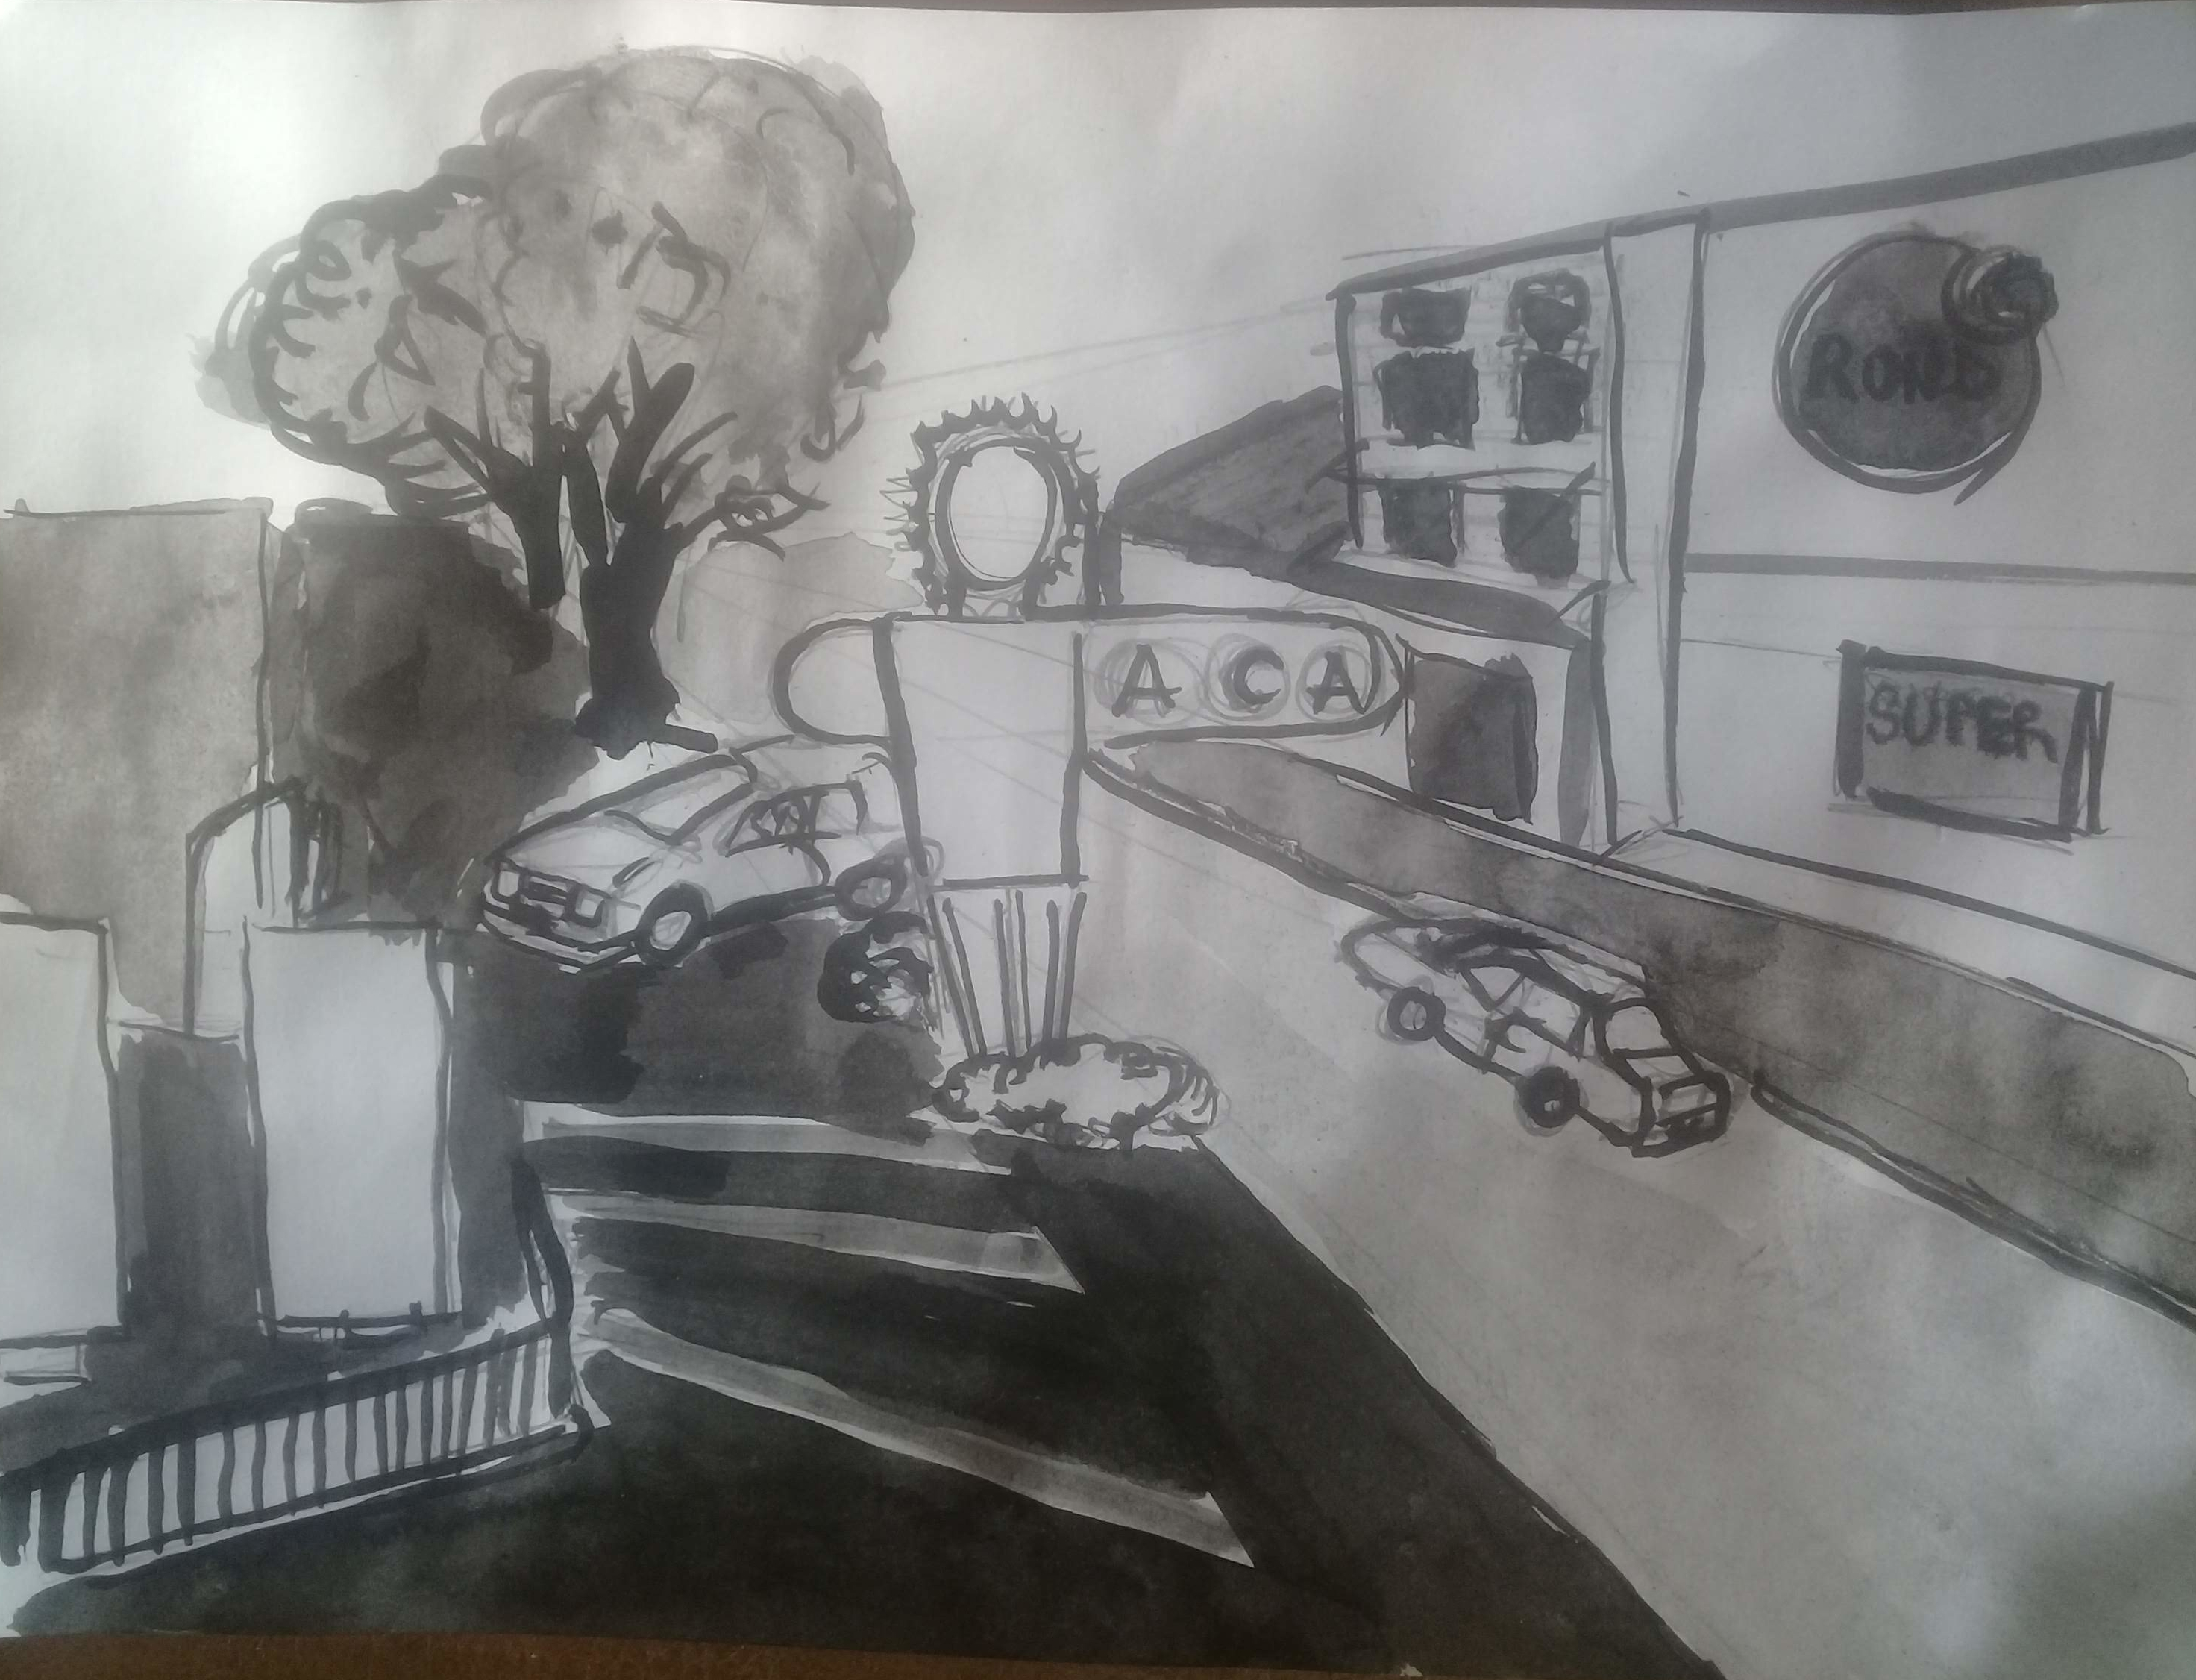
\includegraphics[width=\paperwidth,height=\paperheight,angle=0]{Estacion_servicio}};
	
\end{tikzpicture}


\newpage
\begin{tikzpicture}[remember picture, overlay]
	\node [inner sep=0pt, minimum width=\paperwidth, minimum height=\paperheight] at (current page.center) {
\includegraphics[width=\paperwidth,height=\paperheight,angle=0]{paper11}};
\end{tikzpicture}
ME MOVÍ CON CUIDADO POR LA ESTACIÓN DE SERVICIO, IBA CORRIENDO 	DE UN LUGAR SEGURO A OTRO CON PRECAUCIÓN FELINA. 

DE PRONTO, VINO UN RUIDO MUY ESTRIDENTE DESDE LA AVENIDA. ME ASUSTÉ MUCHÍSIMO Y DE UN SALTO ME ESCONDÍ EN EL ARBUSTO JUNTO AL CARTEL. HABÍA FRENADO MUY FUERTE UNA CAMIONETA, PARA EVITAR UN CHOQUE CON UN AUTO. 

DESDE LAS VENTANILLAS, LOS CONDUCTORES COMENZARON A GRITARSE PALABRAS QUE NO HABÍA ESCUCHADO NUNCA$\ldots$ O ALGUNA SE PARECÍA A ESA QUE HABÍA RECIBIDO DESPUÉS DE HABER ARROJADO AQUEL RETRATO DESDE LA BIBLIOTECA. EN FIN, UNA VEZ QUE SE CALMÓ EL TRÁNSITO NUEVAMENTE, SALÍ DE MI ARBUSTO Y ME AVENTURÉ MÁS ALLÁ.

LLEGUÉ A UN NEGOCIO QUE ESTABA CUBIERTO DE PEGATINAS, Y QUE TENÍA UN CURIOSO FAROL REDONDO CON UNA CRUZ GRANDE SOBRE SU PUERTA.




\newpage
\begin{tikzpicture}[remember picture, overlay]
	\node [inner sep=0pt, minimum width=\paperwidth, minimum height=\paperheight] at (current page.center) {
\includegraphics[width=\paperwidth,height=\paperheight,angle=0]{paper11}};
	\node [inner sep=0pt,  minimum height=\paperheight,xshift=0\textwidth,yshift=.1\textheight] at (current page.center){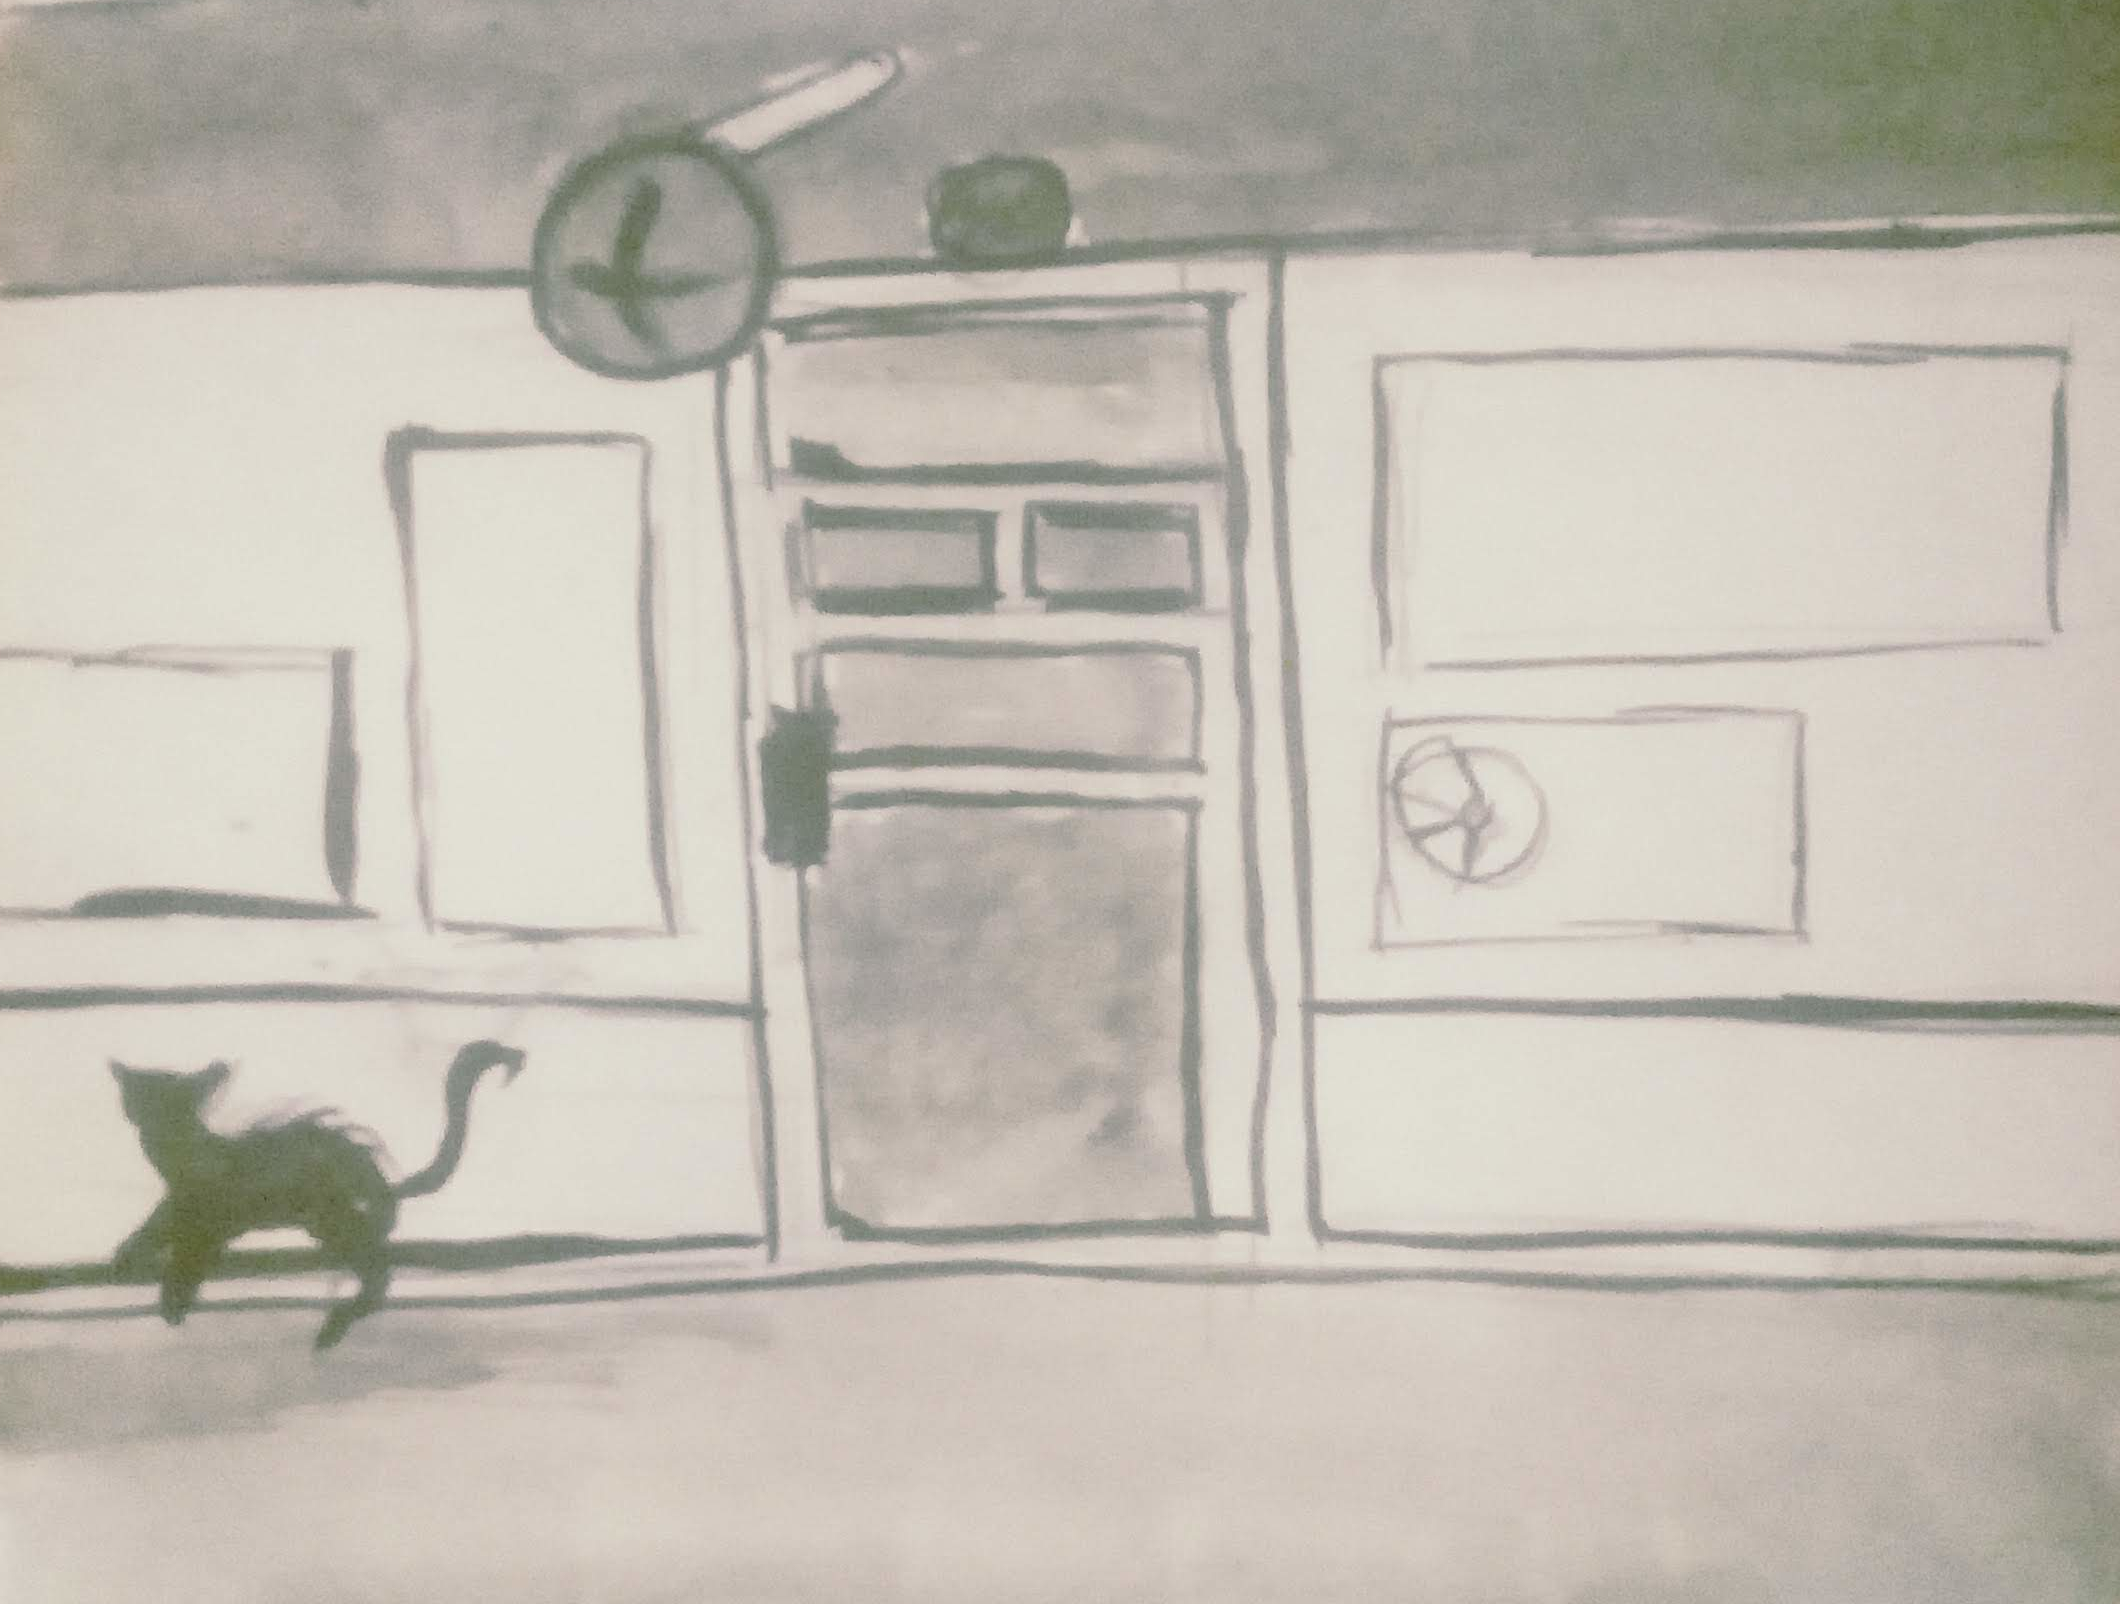
\includegraphics[height=.9\paperheight,angle=0]{farmacia}};
	
\end{tikzpicture}

\vspace{.8\textheight}
¡UN FUERTE  PERFUME ME HIZO RECORDAR A LA VETERINARIA!	




\newpage
\begin{tikzpicture}[remember picture, overlay]
	\node [inner sep=0pt, minimum width=\paperwidth, minimum height=\paperheight] at (current page.center) {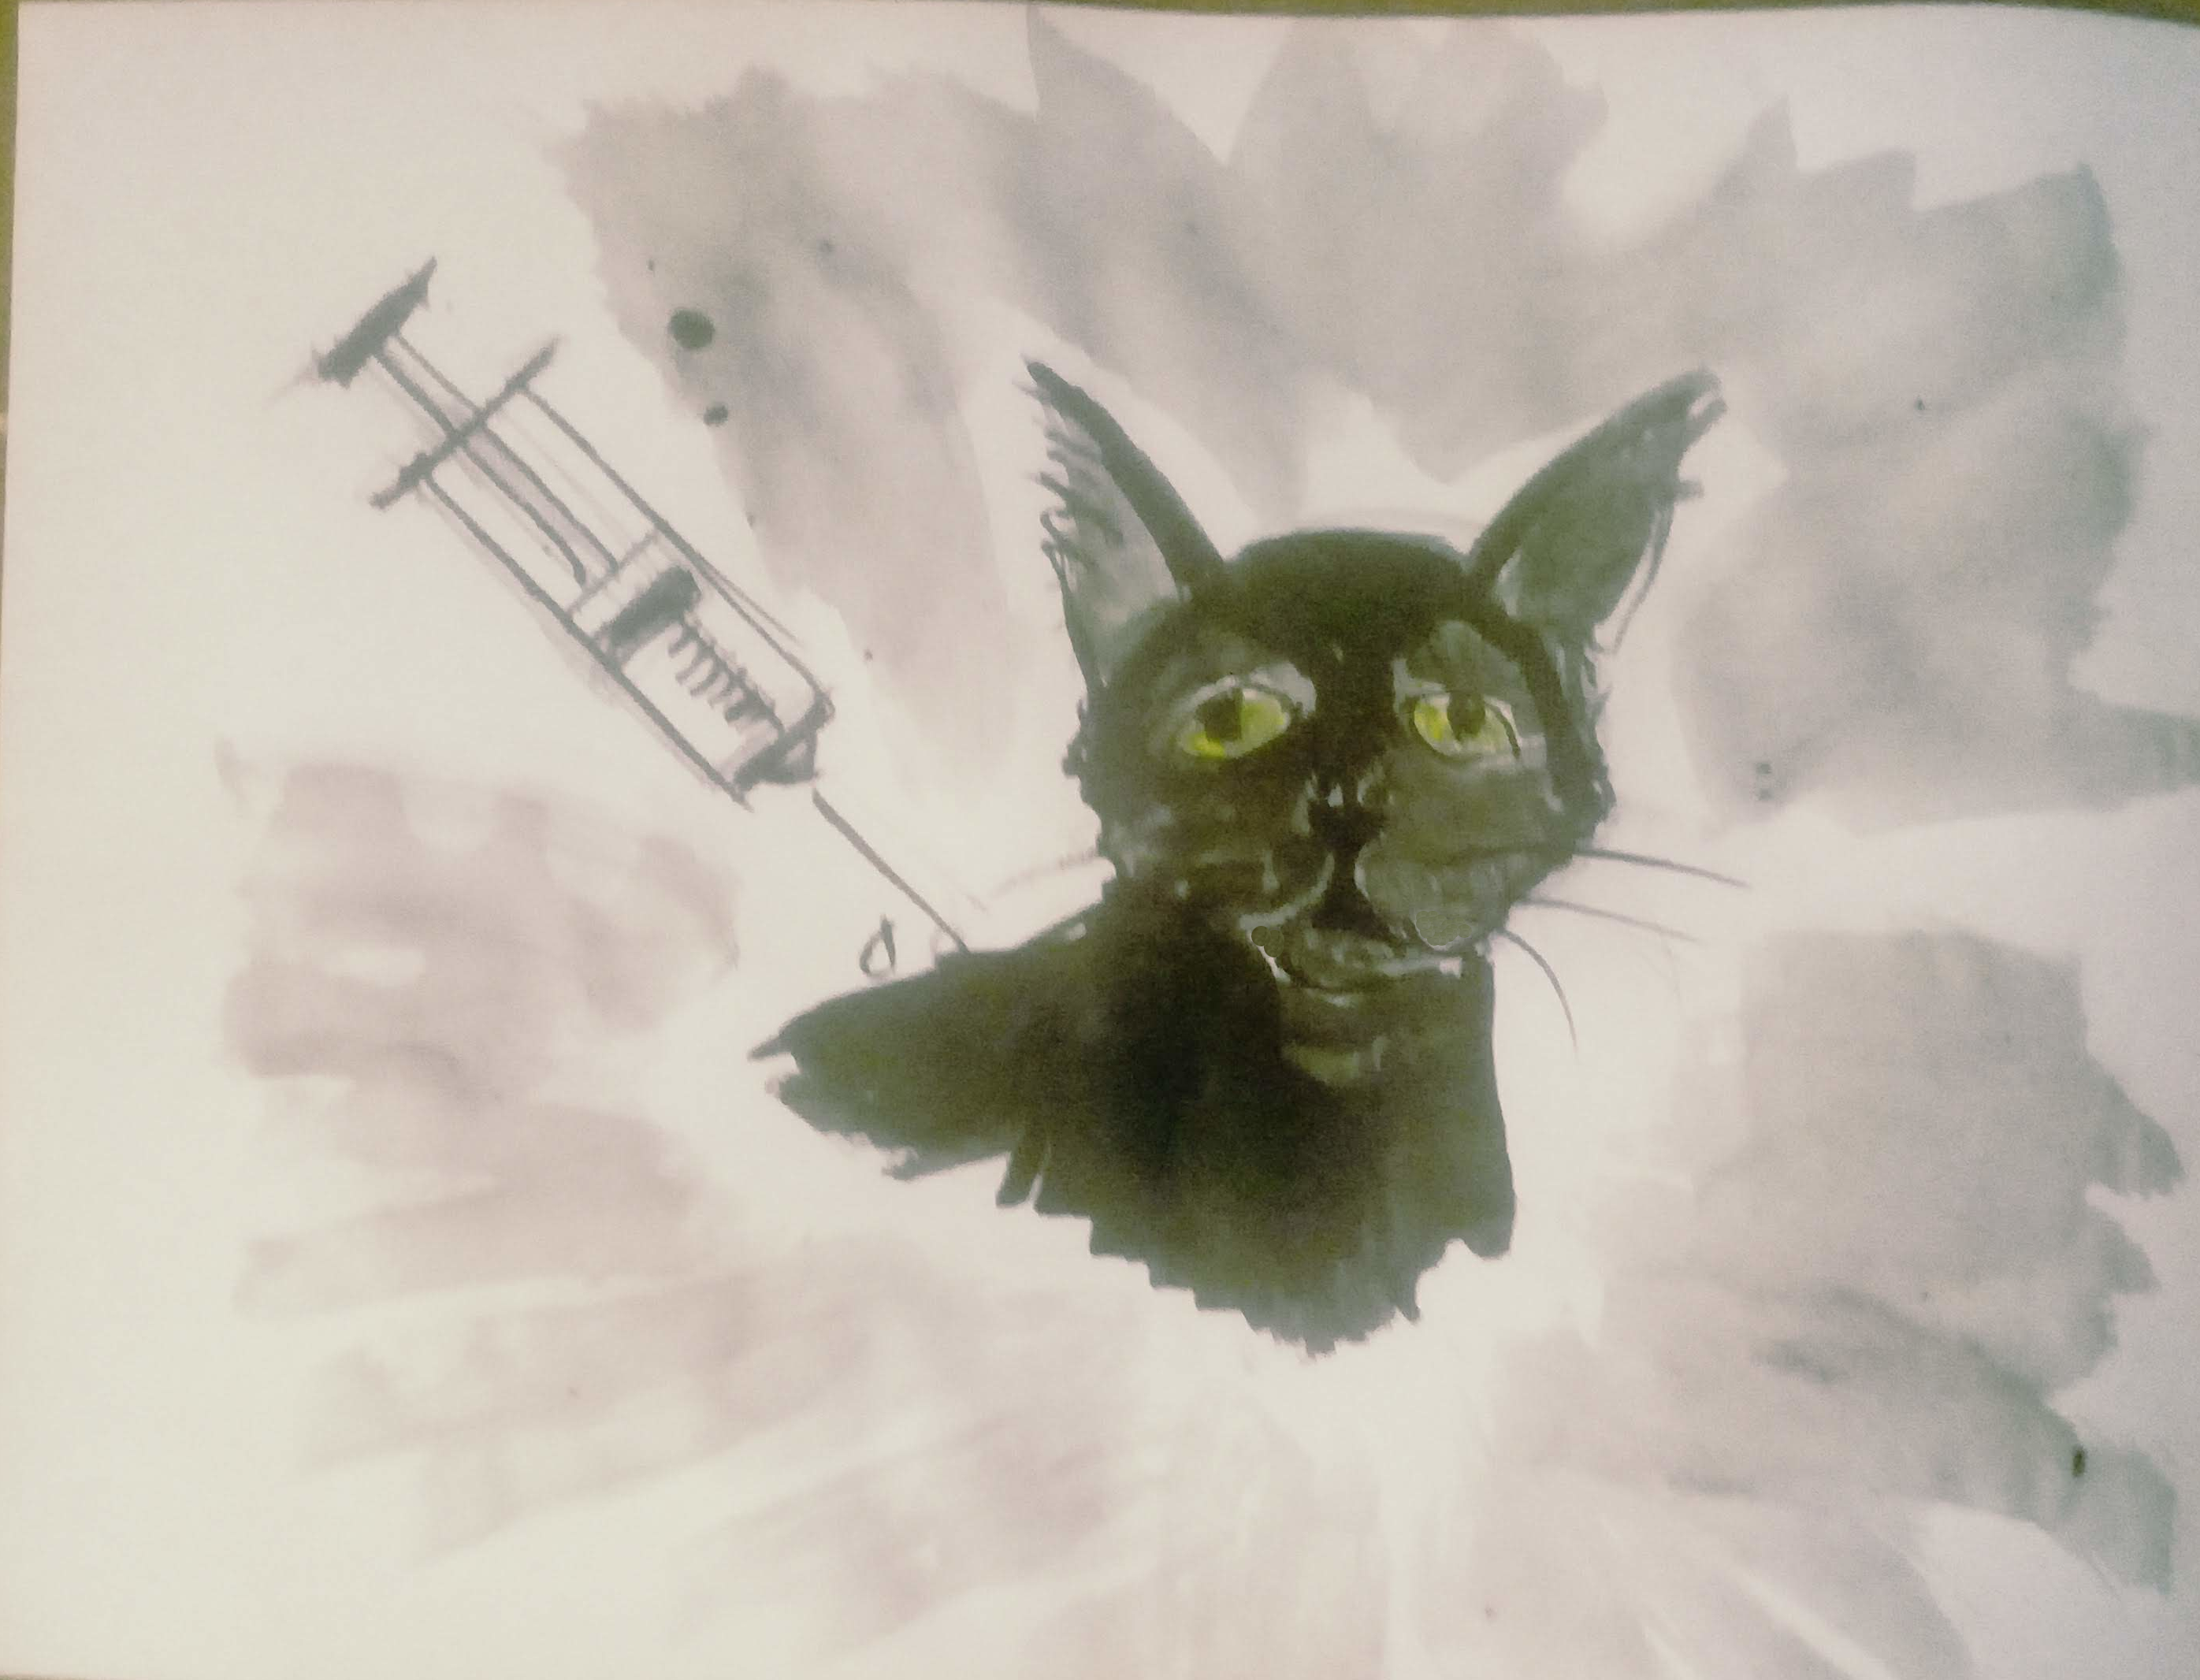
\includegraphics[width=\paperwidth,height=\paperheight,angle=0]{recuerdos_veterinaria}};
\end{tikzpicture}
\vspace{.8\textheight}
¡NO ERAN LOS MEJORES RECUERDOS DE MI NIÑEZ!	

OLOR A ALCOHOL Y A MEDICAMENTOS




\newpage
\begin{tikzpicture}[remember picture, overlay]
	\node [inner sep=0pt, minimum width=\paperwidth, minimum height=\paperheight,opacity=.5] at (current page.center) {
\includegraphics[width=\paperwidth,height=\paperheight,angle=0]{paper8}};
\end{tikzpicture}
NADA BUENO ESPERARÍA DE UN LUGAR ASÍ, Y ANTES DE RETOMAR MI CAMINO, ESCUCHO UNA INCONFUNDIBLE VOZ FELINA CON UN DELICADO ``MIAU``. VUELVO A MIRAR DENTRO DEL NEGOCIO Y TRAS UNAS CALCOMANÍAS VI APARECER UN ROSTRO GATUNO Y UN PORTE DE FINA ESTAMPA. CON SUAVIDAD ESCALÓ UNAS CAJAS Y ALGO DE ARRIBA ME VOLVIÓ A LLAMAR CON SU ``MIAU``

- HOLA JOVENCITO, NO TE CONOCÍA$\ldots$ ¿SOS NUEVO EN EL BARRIO?

EMPECÉ A PENSAR QUE TODOS LOS GATOS DEL BARRIO SE CONOCEN$\ldots$

- NO, SI, $\ldots$ EN REALIDAD ES MI PRIMERA SALIDA A LA CALLE.




\newpage
\begin{tikzpicture}[remember picture, overlay]
	\node [inner sep=0pt, minimum width=\paperwidth, minimum height=\paperheight,opacity=.5] at (current page.center) {
\includegraphics[width=\paperwidth,height=\paperheight,angle=0]{paper3}};
\end{tikzpicture}
MIRÉ SU CARA DE UN TONO GRIS ATERCIOPELADO Y OJOS DE COLOR  ESMERALDA. LLEVABA UN COLLAR MUY DISTINGUIDO PERO NO ALCANZABA A LEER SU NOMBRE. SONREÍA TRANQUILA Y PARECÍA QUE MI PRESENCIA LA DIVERTÍA.

- ¡AH! ME HACÉS ACORDAR A MIS PRIMERAS SALIDAS, ¡QUÉ EMOCIONES AQUELLAS! EN ESTA AVENIDA PASAN MUCHAS COSAS, DEBÉS SER PRECAVIDO, PEQUEÑO.

- ¡YA NO SOY TAN PEQUEÑO!, PROTESTÉ, PRONTO VOY A CUMPLIR UN AÑO, QUE SON COMO 7 AÑOS GATUNOS. 

- ¡ASÍ ME GUSTA! ¡INGENUO Y ORGULLOSO! ¡JA, JA! ¿DESDE DONDE VENÍS?

- MI CASA ESTÁ A UNAS DOS CUADRAS.

- ¿ Y QUÉ TE HIZO QUERER SALIR DE ALLÍ?



\newpage
\begin{tikzpicture}[remember picture, overlay]
	\node [inner sep=0pt, minimum width=\paperwidth, minimum height=\paperheight] at (current page.center) {\includegraphics[width=\paperwidth,height=\paperheight,angle=0]{blaze}};
\end{tikzpicture}
- QUISE ATRAPAR PALOMAS$\ldots$

- ¡PALOMAS! ¡OH, LO ADMITO TAMBIÉN ES UN AÚN UN LEGÍTIMO PASATIEMPO QUE TENGO! 

- ¿DE VERAS?

NO PENSABA QUE UNA GATA TAN 

RESPETABLE COMPARTIERA MI

PASATIEMPO.
\newline\newline	\newline 	

- ¡SÍ! SON CASI IRRESISTIBLES PARA CUALQUIER FELINO. ¿SERÁ PORQUE VUELAN? EN TODO CASO, NO TE CONFÍES NUNCA DE SU ASPECTO, PARECEN MUCHO MÁS TORPES DE LO QUE REALMENTE SON. ES MÁS, DIRÍA QUE SON BASTANTE ASTUTAS.




\newpage
\begin{tikzpicture}[remember picture, overlay]
	\node [inner sep=0pt, minimum width=\paperwidth, minimum height=\paperheight,opacity=1] at (current page.center) {
\includegraphics[width=\paperwidth,height=\paperheight,angle=0]{paper13}};
\end{tikzpicture}
- VEO QUE NO LLEVÁS NI COLLAR NI PLACA -ME DIJO Y AGREGÓ -¿SABE ALGUIEN QUE TE FUISTE DE LA CASA?

- NO, ES VERDAD. VOS SI TENÉS ESE COLLAR Y LA PLACA, AUNQUE NO LLEGO A LEER TU NOMBRE$\ldots$

- MIRA BIEN.

ASÍ FUE QUE PUDE LEER SU NOMBRE, Y ACORDÁNDOME DE SU COLLAR, SE VERÍA ALGO ASÍ. 
\begin{center}
	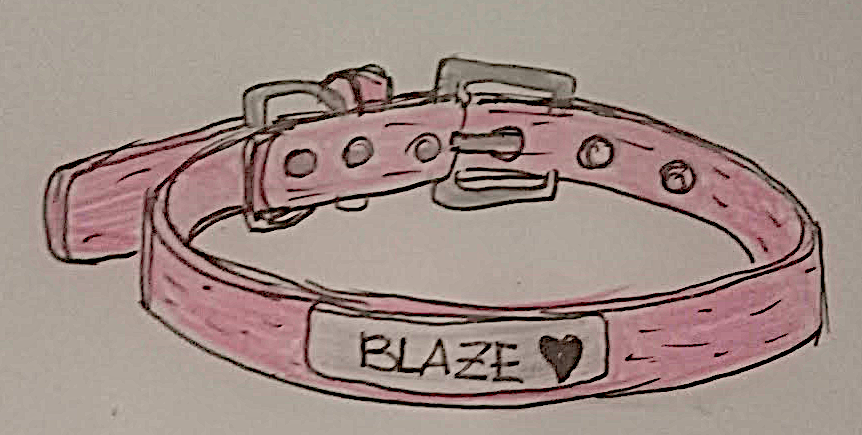
\includegraphics[height=.2\paperheight,angle=0]{collar_blaze}
\end{center}


- ES UN NOMBRE MUY BONITO, LE DIJE. YO ME LLAMO OTTOKO.






\newpage
\begin{tikzpicture}[remember picture, overlay]
	\node [inner sep=0pt, minimum width=\paperwidth, minimum height=\paperheight,opacity=1] at (current page.center) {
\includegraphics[width=\paperwidth,height=\paperheight,angle=0]{paper14}};
	
\end{tikzpicture}
-TENÉS UN NOMBRE MUY ORIGINAL, OTTOKO. TE SIENTA BIEN.

-MUCHAS GRACIAS, BLAZE, EL TUYO ES MUY LINDO Y ME RECUERDA  JUEGOS DE HACE TIEMPO.

-¡SÍ! UN NIÑO ELIGIÓ ESE NOMBRE PARA MÍ POR ESE JUEGO. ¿Y AHORA DONDE VAS A IR, OTTOKO?

-VOY A IR DESCUBRIENDO POCO A POCO.

-ESTÁ BIEN, PERO RECORDÁ QUE NO DEBEMOS SER DEMASIADO CURIOSOS LO GATOS. ¡Y QUE  NOS VEREMOS PRONTO!
\newline	 

FUE ENTONCES QUE SEGUÍ CAMINANDO PARA ENCONTRAR LO QUE LLAMAN UN CORRALÓN. UN LUGAR MUY GRANDE, CON BOLSAS MUY GRANDES Y PESADAS. HABÍA UNAS MAGNÍFICAS ARENAS APILADAS QUE ME INVITARON A INVESTIGAR.



\newpage
\begin{tikzpicture}[remember picture, overlay]
	\node [inner sep=0pt, minimum width=\paperwidth, minimum height=\paperheight] at (current page.center) {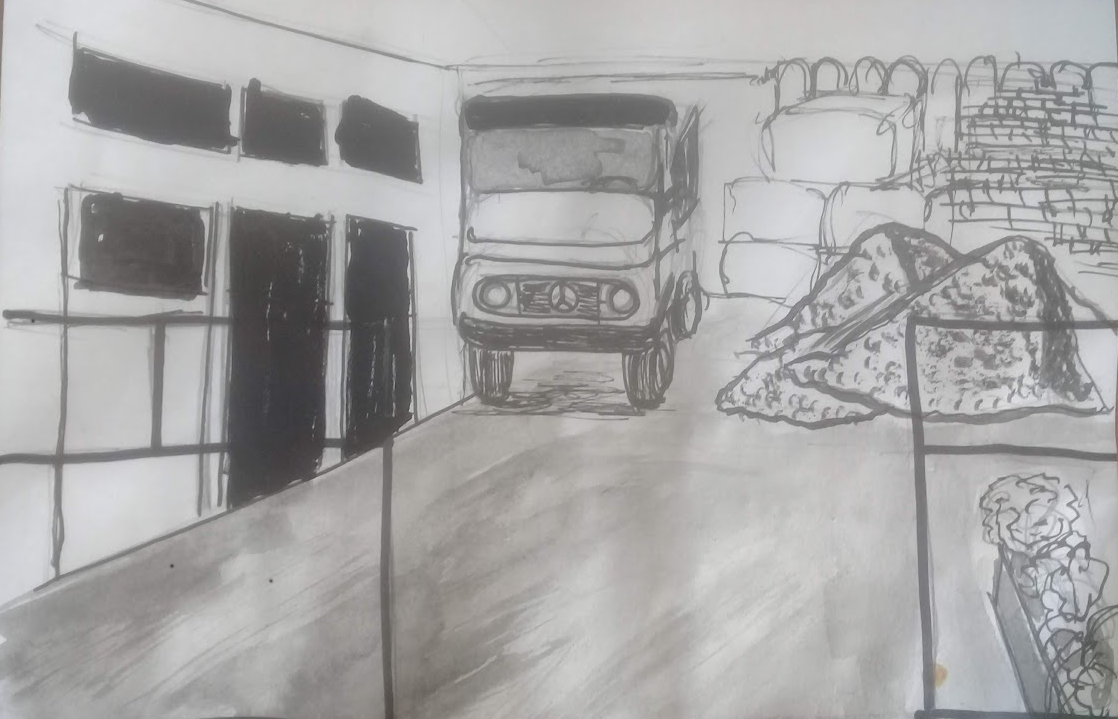
\includegraphics[width=\paperwidth,height=\paperheight,angle=0]{corralon}};
\end{tikzpicture}

\vspace{.8\textheight}
UN LUGAR DE AVENTURAS INESPERADAS.		



\newpage
\begin{tikzpicture}[remember picture, overlay]
	\node [inner sep=0pt, minimum width=\paperwidth, minimum height=\paperheight,opacity=1] at (current page.center) {
\includegraphics[width=\paperwidth,height=\paperheight,angle=0]{paper14}};
	
\end{tikzpicture}
ENTRÉ A INVESTIGAR ESE CORRALÓN. 

EN LA ENTRADA HABÍA HACIA LA DERECHA, MACETAS CON PLANTAS NO MUY LLAMATIVAS. DEL LADO IZQUIERDO, UNAS PUERTAS DABAN A UNAS SALAS OSCURAS QUE PREFERÍ NO VISITAR.

YA HABÍA PASADO ALGÚN TIEMPO DESDE MI SALIDA DE CASA, Y ERA TIEMPO DE IR A LAS PIEDRITAS, O MÁS BIEN DICHO, A LA ARENA, QUE HABÍA A MONTONES DENTRO DE ESE LUGAR.

MÁS ALIVIADO, CONTINUÉ MI RECORRIDO, ENCONTRANDO TAMBIÉN CERCA DE UN CAMIÓN MUCHAS PIEDRAS REDONDEADAS, DE ESAS QUE LLAMAN CANTOS RODADOS. ESTABAN MUY BUENAS PARA JUGAR, UN TAMAÑO ADECUADO PARA MOVERLAS ENTRE MIS PATAS.

- ¿QUE HACE ESE GATO NEGRO ACÁ ADENTRO? - ESCUCHÉ GRITAR UNA VOZ RONCA Y POCO AGRADABLE.

ERA POSIBLE QUE EMPEZARAN ALGUNOS  PROBLEMAS. 


\newpage
\begin{tikzpicture}[remember picture, overlay]
	\node [inner sep=0pt, minimum width=\paperwidth, minimum height=\paperheight] at (current page.center) {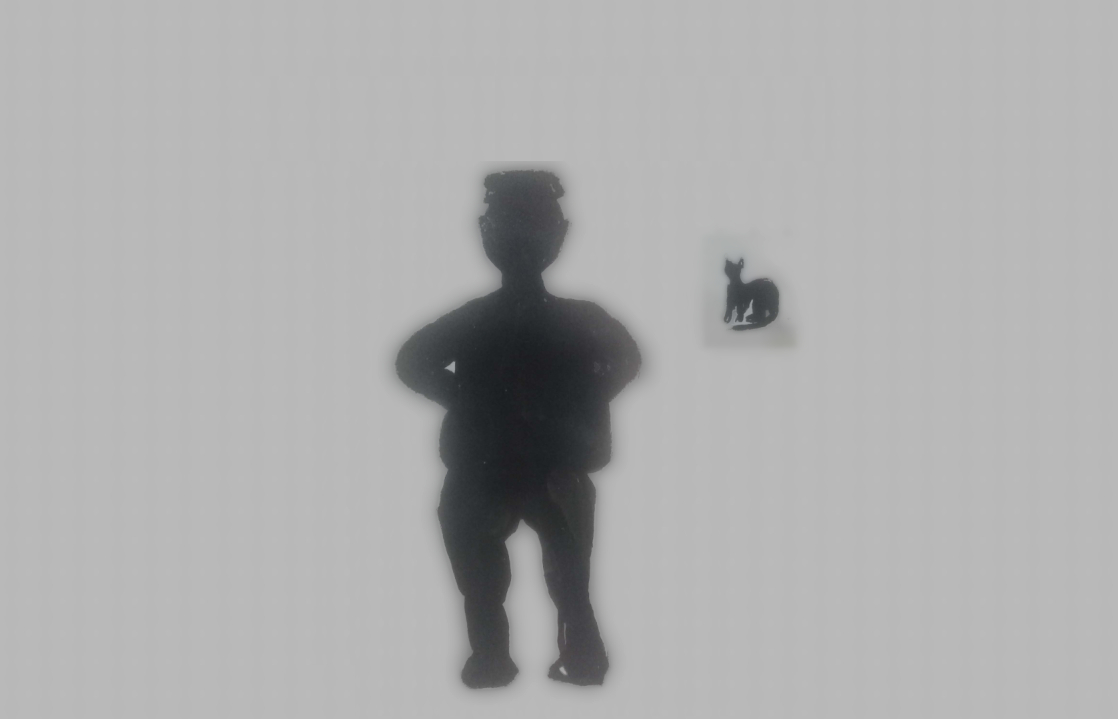
\includegraphics[width=\paperwidth,angle=0]{in_fraganti}};
\end{tikzpicture}

- ME PARECE QUE TENEMOS GATO ENCERRADO, JAJA, DIJO UN HOMBRE MUY CORPULENTO QUE SALIÓ DE UNA DE LAS SALAS.


SE PUSO EN EL MEDIO DE \hspace{.2\textwidth} LA PUERTA DE ACCESO.
\newline\newline

\vspace{.2\textheight}
\begin{minipage}{.3\textwidth}
	SE IBA A COMPLICAR PODER SALIR DE ALLÍ FÁCILMENTE.
\end{minipage}
\hfill
\begin{minipage}{.3\textwidth}
	¿QUÉ HACER?
\end{minipage}






\newpage
\begin{tikzpicture}[remember picture, overlay]
	\node [inner sep=0pt, minimum width=\paperwidth, minimum height=\paperheight,opacity=1] at (current page.center) {
\includegraphics[width=\paperwidth,height=\paperheight,angle=0]{paper14}};
	
\end{tikzpicture}
\begin{LARGE}¡NUESTRO HÉROE ESTÁ EN SERIOS PROBLEMAS EN UN DESCONOCIDO CORRALÓN
	!
	
	
	DECIDE SU ELECCIÓN:
\end{LARGE}
\newline

SI ESCRIBÍS 1, OTTOKO CORRE HACIA LA ALTURA DE LA PILA DE CANTOS RODADOS.

ESCRIBIENDO 2, OTTOKO SE ENFRENTA AGRESIVO CON SUS GARRAS DE PANTERA NEGRA AL CUIDADOR.

SI ESCRIBÍS 3, OTTOKO TRATA DE HACER OJOS DE GATO INOFENSIVO, CONSERVANDO SUS MAÑAS PARA EL MEJOR MOMENTO.
\newline		\newline
\begin{LARGE}
	
	
	ESTÁ EN TUS MANOS SU DESTINO FELINO!!!
\end{LARGE}



\newpage
\begin{tikzpicture}[remember picture, overlay]
	\node [inner sep=0pt, minimum width=\paperwidth, minimum height=\paperheight] at (current page.center) {\includegraphics[width=\paperwidth,angle=0]{ojitos}};
\end{tikzpicture}
\newpage
\begin{tikzpicture}[remember picture, overlay]
	\node [inner sep=0pt, minimum width=\paperwidth, minimum height=\paperheight] at (current page.center) {\includegraphics[width=\paperwidth,height=\paperheight,angle=0]{paper6}};
	
\end{tikzpicture}
IMITÉ A UNO DE MIS  HÉROES PREFERIDOS: EL GATO CON BOTAS.	

MÁS DE UNA VEZ HABÍA VISTO LA PELÍCULA EN DONDE LOGRA GANAR UN PRECIOSO TIEMPO PONIENDO UNA CARA DE TRISTEZA REALMENTE IRRESISTIBLE. TENEMOS UN PÓSTER DE ÉL, QUE PUSIERON ESPECIALMENTE PARA MÍ.

HICE MI MEJOR ESFUERZO PERO CREO QUE EL SEÑOR GUARDIÁN NO PARECÍA MUY ENTERNECIDO. SIGUIÓ ACERCÁNDOSE CON AIRE POCO AMIGABLE HACIA DONDE YO ESTABA. MIENTRAS LO HACÍA, PUDE CALCULAR LA VELOCIDAD QUE PUDIERA TENER. ERA UN HOMBRE MUY PESADO, IMAGINO DE MÁS DE 100 KILOS, ES DECIR 20 VECES APROXIMADAMENTE MI PESO.




\newpage
\begin{tikzpicture}[remember picture, overlay]
	\node [inner sep=0pt, minimum width=\paperwidth, minimum height=\paperheight,opacity=1] at (current page.center) {\includegraphics[width=\paperwidth,height=\paperheight,angle=0]{paper14}};
	
\end{tikzpicture}
RETROCEDÍ HACIA LA MONTAÑITA DE PIEDRAS CANTOS RODADO, QUE PUDE SUBIR CON FACILIDAD, PENSÉ QUE EL SEÑOR IBA A DESANIMARSE PERO CONTINUÓ VINIENDO HACIA MÍ. 

CREO QUE PISÓ UNA PIEDRA Y RESBALÓ UN POCO, Y POR ESO DIJO ALGUNAS MALAS PALABRAS. EN ESOS CASOS, SE ENTIENDE.

SE ACERCABA ENOJADO PERO VEÍA QUE NO IBA A PODER SUBIR LA MONTAÑITA SIN PERDER EL PIE Y CAERSE, VENTAJAS DE SER BIEN LIGERITO, JEJEJE.

IBA A QUEDARME EN MI CIMA TRIUNFAL, CUANDO ESCUCHÉ UN SILBIDO DEL CUIDADOR, Y LUEGO AGREGÓ:

- ¡VENGA PARA ACÁ, MAX!

LO QUE VI A CONTINUACIÓN ME DEJÓ SIN ALIENTO FELINO.



\newpage
\begin{tikzpicture}[remember picture, overlay]
	
	\node [inner sep=0pt, minimum width=\paperwidth, minimum height=\paperheight,opacity=1] at (current page.center) {\includegraphics[width=\paperwidth,height=\paperheight,angle=0]{max_rostro}};
	\node[text width=26cm,xshift=0cm,yshift=0cm] at (current page.center){};
	
\end{tikzpicture}


\newpage
\begin{tikzpicture}[remember picture, overlay]
	
	\node [inner sep=0pt, minimum width=\paperwidth, minimum height=\paperheight,opacity=1] at (current page.center) {\includegraphics[width=\paperwidth,height=\paperheight,angle=0]{paper6}};
\end{tikzpicture}
NUNCA EN MI VIDA HABÍA VISTO UN PERRO TAN GRANDE  Y POR COMO APARECIÓ, PARECÍA MUCHO MÁS RÁPIDO QUE SU DUEÑO. 

COMO BUEN GATO, NO ENTRÉ EN PÁNICO TOTAL, AÚN CUANDO LA SITUACIÓN ERA DE MUCHO PELIGRO. EL PERRO SE ABALANZÓ A TODA VELOCIDAD SOBRE LA PILA DE PIEDRITAS Y SI BIEN TERMINÓ TODO DESPATARRADO, HIZO QUE TODO SE DESPARRAMARA, INCLUYÉNDOME A MÍ,QUE BUSQUÉ OTRO LUGAR PARA REFUGIARME. PUDE TREPAR SOBRE UN CAMIÓN QUE ESTABA ALLÍ. ESTACIONADO, PERO ME PARECIÓ QUE IBA A SER MUY DIFÍCIL ESCAPAR. EL PERRO MAX LADRABA CON FURIA Y RODEABA FURIOSO EL VEHÍCULO.

EL GUARDIÁN, CON SU ANDAR LENTO PERO MACIZO, TENÍA RESERVADA OTRA INQUIETANTE SORPRESA.





\newpage
\begin{tikzpicture}[remember picture, overlay]
	
	\node [inner sep=0pt, minimum width=\paperwidth, minimum height=\paperheight,opacity=1] at (current page.center) {\includegraphics[width=\paperwidth,height=\paperheight,angle=0]{paper6}};
	
\end{tikzpicture}
LO VI IR HACIA UNA CANILLA, DE ESAS TÍPICAS DE JARDÍN, Y TENÍA UNA MANGUERA VERDE CONECTADA. SE PARECÍA A LA QUE TENEMOS EN NUESTRO PATIO, CON LAS QUE SE RIEGAN LAS PLANTAS Y A VECES JUEGO PERSIGUIENDO PEQUEÑOS CHORROS. NUNCA ME TIRAN AGUA PERO ES ALGO MUY DESAGRADABLE ASÍ QUE ME IMAGINÉ QUE ES LO QUE IBA HACER EL SEÑOR ENOJADO.

-AHORA SÍ VAS A VER LO QUE ES BUENO, DE ESTA MOJADURA NO TE ESCAPARÁS, ME DIJO.

EL PERRO SEGUÍA LADRANDO Y YO ARRIBA DE ESE CAMIÓN PASABA UN MOMENTO MUY DIFÍCIL. PENSÉ QUE ERA MUY INJUSTO DOS CONTRA UNO, Y ENCIMA DOS ENORMES MAMÍFEROS. PENSÉ EN LLAMAR A MI PAPÁ, ÉL ME RESCATARÍA SIN DUDAR. ME ARREPENTÍA DE HABERME IDO, MAULLÉ UN TANTO TRISTE.



\newpage
\begin{tikzpicture}[remember picture, overlay]
	
	\node [inner sep=0pt, minimum width=\paperwidth, minimum height=\paperheight,opacity=1] at (current page.center) {\includegraphics[width=\paperwidth,height=.9\paperheight,angle=0]{manguera_patio}};
	
	
\end{tikzpicture}
\newpage
\begin{tikzpicture}[remember picture, overlay]
	
	\node [inner sep=0pt, minimum width=\paperwidth, minimum height=\paperheight,opacity=1] at (current page.center) {\includegraphics[width=\paperwidth,height=\paperheight,angle=0]{manguera_corralon}};
	\node[text width=.9\textwidth,xshift=0cm,yshift=.25\textheight] at (current page.center){ESTE MOMENTO ERA  MUY DISTINTO. ¡PERO NO IBA A RENDIRME!
	};
	
\end{tikzpicture}
\newpage
\begin{tikzpicture}[remember picture, overlay]
	
	\node [inner sep=0pt, minimum width=\paperwidth, minimum height=\paperheight,opacity=1] at (current page.center) {\includegraphics[width=\paperwidth,height=\paperheight,angle=0]{paper9}};
\end{tikzpicture}
FUE ENTONCES QUE ESCUCHÉ, DESPUÉS DEL MÍO, OTRO MAULLIDO QUE DESORIENTÓ AL SEÑOR Y A SU PERRO. VENÍA DESDE LA PUERTA.

- MIRÁ, ¡SI ES LA GATITA DE LA FARMACIA DEL AL LADO! ¿VOS TAMBIÉN QUERÉS MOJARTE, PRINCESA?

¡ERA BLAZE! MAULLABA PARA LLAMAR LA ATENCIÓN Y DARME UNA OPORTUNIDAD DE ESCAPE. PERO EL MAX VOLVIÓ A RODEAR EL CAMIÓN Y LADRAR.

DECIDIDA, BLAZE EMPEZÓ A MALTRATAR ALGUNAS PLANTAS DE LA ENTRADA E HIZO QUE EL GUARDIÁN FUERA A ECHARLA. EN ESE MISMO MOMENTO, APARECIÓ POR ENCIMA DE LA PARED MEDIANERA DE ATRÁS, AKIS, EL GATO DE DOS COLORES. 

- ¡ESA NO ES FORMA DE TRATAR A UN FELINO TAN JOVEN!, PROTESTÓ ARQUÉANDOSE Y SACANDO FILOSAS GARRAS.


\newpage
\begin{tikzpicture}[remember picture, overlay]
	
	\node [inner sep=0pt, minimum width=\paperwidth, minimum height=\paperheight,opacity=1] at (current page.center) {\includegraphics[width=\paperwidth,height=\paperheight,angle=0]{blaze_enojada}};
	\node[text width=24cm,xshift=0cm,yshift=8cm] at (current page.center){¡LLEGABAN LOS REFUERZOS GATUNOS!
	};
	
\end{tikzpicture}
\newpage
\begin{tikzpicture}[remember picture, overlay]
	
	\node [inner sep=0pt, minimum width=\paperwidth, minimum height=\paperheight,opacity=1] at (current page.center) {\includegraphics[width=\paperwidth,height=\paperheight,angle=0]{paper12}};
	
\end{tikzpicture}
ASÍ FUE QUE AKIS DESDE EL FONDO Y BLAZE DESDE EL FRENTE, CONFUNDIERON A QUIENES ME HABÍAN ATRAPADO. 

- ¡VAMOS, OTTOKITO!, DIJO AKIS, ¡RÁPIDO, SALÍ DE ESE CAMIÓN Y SUBÍ ESA PARED!

COMO EL PERROTE MAX LO PERSEGUÍA A ÉL, Y EL GUARDIÁN HABÍA IDO CON SU MANGUERA TRAS BLAZE, FUE EN UN INSTANTE QUE ME ESCURRÍ Y ALCANCÉ LA PARED DEL FONDO, MUCHO MÁS SEGURO.

- ¡LISTO, BLAZE, YA PODÉS VOLVERTE!

NI UNA GOTA DE AGUA HABÍA TOCADO A NUESTRA HEROÍNA, QUIEN SE HABÍA LLEVADO DE TROFEO ALGUNOS PEDAZOS DE HOJAS DE ESAS PLANTAS RARAS QUE LLAMAN ``ESPADA DE SAN JORGE". SIEMPRE ME PARECIERON BASTANTE FEAS, ALGO PARECIDAS A LOS PEPINOS.



\newpage
\begin{tikzpicture}[remember picture, overlay]
	
	\node [inner sep=0pt, minimum width=\paperwidth, minimum height=\paperheight,opacity=1] at (current page.center) {\includegraphics[width=\paperwidth,height=\paperheight,angle=0]{paper12}};
\end{tikzpicture}
UNA VEZ TODOS A SALVO, SI BIEN LOS HUMANOS ESCUCHARÍAN MAULLIDOS Y LADRIDOS, YO ENTENDÍ COMO AKIS LE REPROCHÓ A MAX AGARRARSELAS CON UN GATITO JOVEN E INEXPERTO COMO YO.

- TENGO QUE OBEDECER AL DUEÑO, YO, SE JUSTIFICÓ MAX.

- ¡AH, NO! HAY LÍMITES PARA OBEDECER, ASÍ NO HABLA UN VALIENTE, DIJO AKIS.

- ME GUSTARÍA VER CUAN VALIENTE SERÍAS ACÁ ABAJO, GATO MATRERO.

- TENÉS RAZÓN, PUES. VAYA UNA ROCIADA DE POCA VALENTÍA.	
Y ASÍ NOMÁS, EL GATO HIZO PIS DESDE LO ALTO DEL MURO, ANTE LOS FURIOSOS LADRIDOS DEL PERRO, Y EL GRANDOTE GUARDÍAN QUE NOS MALDIJO. HABÍA VISTO YO ALGUNOS DOCUMENTALES EN LA TELE DE GRANDES FELINOS QUE HACÍAN PIS DE ESA MANERA EN LA JUNGLA. ADMIRÉ A MI NUEVO AMIGO.



\newpage
\begin{tikzpicture}[remember picture, overlay]
	
	\node [inner sep=0pt, minimum width=\paperwidth, minimum height=\paperheight,opacity=1] at (current page.center) {\includegraphics[width=\paperwidth,height=\paperheight,angle=0]{paper11}};
	
\end{tikzpicture}
MAX LADRÓ Y PRONTO EL SEÑOR CON SU MANGUERA SE ACERCARON Y NOS FUIMOS CON UNOS BUENOS SALTOS GATUNOS. CAMINANDO POR LAS PAREDES Y TECHOS LLEGAMOS A LA CALLE NAVARRO, DONDE AGITADO PERO YA A SALVO LE DIJE A AKIS:

- MUCHAS GRACIAS POR AYUDARME, FUE INESPERADO Y MILAGROSO QUE APARECIERAN.

- TAMBIÉN PODRÁS DARLE LAS GRACIAS A BLAZE, QUIEN ME PIDIÓ QUE VINIERA.

- ¿OH, SI ?	,DIJE YO, Y JUSTO EN ESE MOMENTO SE NOS UNIÓ LA BELLA GATA GRIS DE LA FARMACIA.

- ¿COMO ANDAN MUCHACHOS? ¡TE METISTE EN FLOR DE PROBLEMAS, OTTOKO! PERO LA VERDAD ES QUE ESE TIPO Y EL PERRO MAX EXAGERARON EN CAZARTE ASÍ.



\newpage
\begin{tikzpicture}[remember picture, overlay]
	
	\node [inner sep=0pt, minimum width=\paperwidth, minimum height=\paperheight,opacity=1] at (current page.center) {\includegraphics[width=\paperwidth,height=\paperheight,angle=0]{amigos1}};
\end{tikzpicture}
MÁS TRANQUILO CON MIS NUEVOS AMIGOS.



\newpage
\begin{tikzpicture}[remember picture, overlay]
	
	\node [inner sep=0pt, minimum width=\paperwidth, minimum height=\paperheight,opacity=1] at (current page.center) {\includegraphics[width=\paperwidth,height=\paperheight,angle=0]{paper12}};
	
\end{tikzpicture}

- ¡ME RESCATARON! REALMENTE NO SABÍA COMO IBA A PODER LIBRARME YO SOLO. ¿POR QUÉ LO HICIERON?

- NO ES NADA, PEQUEÑO, ALGO DE SOLIDARIDAD FELINA, DIJO AKIS.

- ASÍ ES, ES LO QUE CORRESPONDE, OTTOKO. NO PODÍAMOS DEJAR QUE ESE ANIMAL Y SU PERRO PATOTERO, TE HICIERAN DAÑO, AGREGÓ BLAZE.

- Y ¿POR QUÉ PENSARON EN MI?

- YO QUE VIVO EN LA FARMACIA YA HABÍA ESCUCHADO DE EPISODIOS ASÍ, ENTONCES ESPIÉ Y EN CUANTO VI  QUE HABRÍA PROBLEMAS FUI A PEDIRLE AYUDA A AKIS QUE ESTABA EN SU ÁRBOL PREFERIDO.

- ES DECIR, SIGUIÓ BLAZE, UN GATO INEXPERTO, UN ARENERO GIGANTE,  DOS GUARDIANES MALANDRINES PUEDEN PRODUCIR UNA SITUACIÓN HORRIBLE: ¡GATO MOJADO!


\newpage
\begin{tikzpicture}[remember picture, overlay]
	
	\node [inner sep=0pt, minimum width=\paperwidth, minimum height=\paperheight,opacity=1] at (current page.center) {\includegraphics[width=\paperwidth,height=\paperheight,angle=0]{paper6}};
	
\end{tikzpicture}
PARA NO QUEDAR MUY INEXPERTO, ME PERMITÍ COMENTAR:

- A MI ME GUSTA EL AGUA PERO CUANDO LA VOY A BUSCAR YO, NO CUANDO ME LLEGA   DE MOJARME DESDE MANGUERAS, ROCIADORES, VASOS$\ldots$

- ASÍ ES, TODO ESTÁ EN LA INTENCIÓN. Y TENÉS QUE ACORDARTE LA PRÓXIMA  VEZ LO QUE TE DIJE SOBRE NUESTRA CURIOSIDAD.

- SÍ, SEÑORA BLAZE. AUNQUE ES MUY DIFÍCIL DE RESISTIR NUESTRO INSTINTO GATUNO.

- LO IMPORTANTE, DIJO CON AIRE EXPERIMENTADO Y SENSATO AKIS, ES PODER CONTAR CON UNA VÍA EXTRA DE ESCAPE.

- ¿COMO ES ESO, EXACTAMENTE?, PREGUNTÉ.

- ES SENCILLO, ANTES DE IR A UNA SALA, FIJATE QUE PUEDAS SALIR POR OTRO LUGAR ADEMÁS DE LA PUERTA POR LA QUE ENTRÁS.


\newpage
\begin{tikzpicture}[remember picture, overlay]
	
	\node [inner sep=0pt, minimum width=\paperwidth, minimum height=\paperheight,opacity=1] at (current page.center) {\includegraphics[width=\paperwidth,height=.9\paperheight,angle=0]{embolsado}};
	\node[text width=.9\textwidth,xshift=0cm,yshift=-.2\textheight] at (current page.center){\textcolor{yellow}{¿QUIÉN NO DISFRUTA ENTRANDO A UNA BUENA BOLSA?}
	};
	
	
\end{tikzpicture}
\newpage
\begin{tikzpicture}[remember picture, overlay]
	
	\node [inner sep=0pt, minimum width=\paperwidth, minimum height=\paperheight,opacity=1] at (current page.center) {\includegraphics[width=\paperwidth,height=\paperheight,angle=0]{paper3}};
	
\end{tikzpicture}
ASÍ ES, AFIRMÓ BLAZE, LOS GATOS TENEMOS ATRACCIÓN POR LAS TRAMPAS$\ldots$ TAL VEZ SEA PORQUE CASI SIEMPRE PODEMOS ESCAPAR DE ELLAS.

- HOY SI USTEDES NO ESTABAN, NO SÉ SI LO HUBIESE LOGRADO, CONFESÉ.

- IRÁS APRENDIENDO -DIJO AKIS- ¿QUE VAS A HACER AHORA, MUCHACHO ?

- CREO QUE FUE UNA GRAN EMOCIÓN POR HOY, TAL VEZ DEBA VOLVER.

- SI,  OTTOKO, SEGURAMENTE ALGUIEN ESTARÁ PREOCUPADO SI NO TE VE EN CASA, ACONSEJÓ BLAZE.

- TENÉS RAZÓN, LOS VEO PRONTO, ¡MIS AMIGOS!, LES DIJE Y ME DESPEDÍ PARA VOLVER CAMINANDO POR LA CALLE NAVARRO.

- ¡HASTA PRONTO, OTTOKO! -SALUDARON AL UNÍSONO.

\newpage
\begin{tikzpicture}[remember picture, overlay]
	\node [inner sep=0pt, minimum width=\paperwidth, minimum height=\paperheight,opacity=1] at (current page.center) {\includegraphics[width=\paperwidth,height=0.93\paperheight,angle=0]{gato_mojado_1}};
	
	
	\node[text width=.7\textwidth,xshift=-.15\textwidth,yshift=-.4\textheight] at (current page.center){\textcolor{yellow}{PARA QUE VEAN QUE, CUANDO QUIERO, ME MOJO LOS BIGOTES Y EL ROSTRO. ¡ES MUY TENTADOR CADA VEZ QUE VEO UN CHORRITO DE AGUA!}};	
\end{tikzpicture}
\newpage
\begin{tikzpicture}[remember picture, overlay]
	\node [inner sep=0pt, minimum width=\paperwidth, minimum height=\paperheight,opacity=1] at (current page.center) {\includegraphics[width=\paperwidth,height=0.93\paperheight,angle=0]{navarro}};
\end{tikzpicture}

\newpage
\begin{tikzpicture}[remember picture, overlay]
	
	\node [inner sep=0pt, minimum width=\paperwidth, minimum height=\paperheight,opacity=1] at (current page.center) {\includegraphics[width=\paperwidth,height=\paperheight,angle=0]{paper6}};
\end{tikzpicture} 
VOLVÍA ENTONCES POR LA CALLE NAVARRO, PENSANDO EN MIS RECIENTES HALLAZGOS. NO PODÍA DECIR QUE SE TRATABA AÚN DE UNA GLORIOSA AVENTURA, AÚN NO HABÍA LLEGADO A ESE PUNTO, PERO SÍ ME SIRVIÓ LA EXPERIENCIA PARA CONOCER UN POCO COMO SON LAS COSAS FUERA DE CASA. Y TAMBIÉN PARA QUERER AÚN MÁS A MI CASA, A MIS PLANTAS, AL LUGAR TRANQUILO DONDE TOMO SOL, DONDE AFILO MIS GARRAS. Y DONDE TOMO AGUA Y COMO MIS DELICIOSAS CROQUETAS. HABÍA CONOCIDO NUEVOS AMIGOS, Y OTROS PERSONAJES QUE MÁS BIEN EVITAR, Y CASI QUE ME GUSTARÍA PODER HABLAR Y CONTARLE A MIS SERES QUERIDOS TODO LO QUE HABÍA PASADO.

ME AGUARDABA UN BUEN DESCANSO GATUNO Y PRONTO EJERCITARME PARA NUEVAS EXPEDICIONES.



\newpage
\begin{tikzpicture}[remember picture, overlay]
	\node [inner sep=0pt, minimum width=\paperwidth, minimum height=\paperheight,opacity=1] at (current page.center) {\includegraphics[width=\paperwidth,height=0.93\paperheight,angle=0]{paper16.png}};
	
	\node [inner sep=0pt, minimum width=\paperwidth, minimum height=\paperheight,opacity=1] at (current page.center) {\includegraphics[width=\paperwidth,height=0.93\paperheight,angle=0]{de_vuelta}};
	
	
	\node[text width=.8\textwidth,xshift=.5\textwidth,yshift=-.0\textheight] at (current page.center){\textcolor{yellow}{\hspace{.1\textwidth }DE VUELTA}
		
		\textcolor{yellow}{		\hspace{1cm} Y UN MERECIDO }
		
		\textcolor{yellow}{			 DESCANSO EN CASA.}};	
\end{tikzpicture}


\newpage
\begin{tikzpicture}[remember picture, overlay]
	
	\node [inner sep=0pt, minimum width=\paperwidth, minimum height=\paperheight,opacity=1] at (current page.center) {\includegraphics[width=\paperwidth,height=0.93\paperheight,angle=0]{cariño}};
	
	\node[text width=12cm,xshift=5cm,yshift=-8.5cm,fill=white,draw=black] at (current page.center){ ¡NI SE IMAGINÓ DONDE ESTUVE!};
	
	
\end{tikzpicture}
